\documentclass[a4j, 11pt]{jreport}
% START:共通設定&共通パッケージ読み込み(基本変更しない)
\renewcommand{\baselinestretch}{1.4}
\setlength{\oddsidemargin}{-0mm}
\setlength{\textwidth}{16cm}
\setlength{\topmargin}{-1.5cm}
\setlength{\textheight}{24cm}
\setlength{\baselineskip}{2cm}
\special{pdf: minorversion=7}    % 出力するPDFのバージョンを指定
\usepackage{ifthen}              % if文制御用
\usepackage[dvipdfmx]{graphicx}
\usepackage{amsmath}             % 数式用
\usepackage{array}               % 数式での場合分け用
\usepackage{url}                 % URL表示用
\usepackage{here}                % [H]用
\usepackage[dvipdfmx]{hyperref}  % 全体像把握&簡易移動のため
\usepackage{pxjahyper}           % 日本語のしおり(ブックマーク)表示用
\hypersetup{pdfborder = {0 0 0}} % hyperrefリンクの囲みを消す
\pagenumbering{roman}            % ページ番号をアラビア数字に変更
\newcounter{fiscal_year}         % 卒業年度計算用
\setcounter{fiscal_year}{\the\year}
\ifthenelse{\the\month < 4}{
	% 年明けから3月までは年-1にする
	\addtocounter{fiscal_year}{-1}
}{}


% END:共通設定&共通パッケージ読み込み(基本変更しない)


% START:ユーザ設定&ユーザパッケージ読み込み---------
\usepackage{caption}
\captionsetup[table]{justification=centering}
\captionsetup[figure]{justification=centering}
\captionsetup{compatibility=false}

\usepackage{paralist}



% END:ユーザ設定&ユーザパッケージ読み込み-----------


\begin{document}
% START:タイトル
\begin{titlepage}\Large ~
{\normalsize \the\value{fiscal_year} 年度卒業}
\vfill
\begin{center}

% START: 論文の種類-------------------------------
{\Huge 修士論文}
% {\Huge 卒業論文}
% END: 論文の種類---------------------------------
\end{center}
\begin{center}

% START: 日本語タイトル---------------------------
空間解像度差のあるデータセットを用いた深層学習による銀河形状分類精度
% END: 日本語タイトル-----------------------------
\end{center}
\begin{center}

% START: 英語タイトル-----------------------------
日本語タイトル暫定版なため,ここ英語タイトルも未完!
% END: 英語タイトル-------------------------------
\end{center}
\vfill
\begin{center}
\begin{tabular}{|c|l|}
\hline

% START: 論文の種類-------------------------------
所属 & 新潟大学自然科学研究科 電気情報工学専攻・飯田佑輔研究室 \\
% 所属 & 新潟大学工学部情報工学科・林隆史研究室 \\
% END: 論文の種類---------------------------------
\hline

% START: 在籍番号---------------------------------
在籍番号 & F20C026D \\
% END: 在籍番号-----------------------------------
\hline

% START: 論文著者---------------------------------
氏名 & 本間 裕也 \\
% START: 論文著者---------------------------------
\hline
\end{tabular}
\end{center}
\vspace{1cm}
\vfill
\end{titlepage}
\pagebreak
\addtocounter{page}{1}
\thispagestyle{empty}  % このページにページ番号を振らない
% END:タイトル

% START:アブストラクト-----------------------------
\chapter*{概要}
日本語のアブストラクト

\chapter*{Abstract}
English Abstract Here

% END:アブストラクト-------------------------------

% START:目次作成
\newpage
\tableofcontents       % 目次作成
\thispagestyle{empty}  % このページにページ番号を振らない
\pagebreak
\pagenumbering{arabic} % ページ番号をアラビア数字に変更
% END:目次作成


% START:本編--------------------------------------
\chapter{はじめに}

\newpage
\chapter{ディープラーニング}
ディープラーニングは機械学習手法の一種であり,人間が学習の指標を決めずとも自ら学習データ内の特徴を捉えながら学習を行っていくアルゴリズムである.この「自ら特徴を見つけ出し学ぶ」という特徴から,膨大な量のデータセットであるビッグデータを学習に用いることで,近年様々なタスクを解決に導ける手法として注目されている.ディープラーニングが近年台頭してきた理由として,Tensorflow, Kerasなどディープラーニングモデルが簡単に構築可能になるライブラリが開発された点,またディープラーニングの学習に用いられるビッグデータが蓄積されてきた点,そして計算機が発達し,これら膨大な容量をもつビッグデータを処理できるほどの処理能力を会得した点などが挙げられる.

第2章では,本論文における銀河形態分類モデルの開発に用いられている,ディープラーニングについて説明を行う.
\section{ディープニューラルネットワーク (ディープラーニング)}
ディープラーニングでは,様々な層で構築された\textbf{モデル}と呼ばれるものを扱う.答えの分かっている学習データを用いてモデルを学習させ,テストデータを用いてモデルの性能検証を行い,そしてモデルを用いて答えの分かっていないデータに対し予測を適用する.
この節では,ディープラーニングの中で最も基本的なモデルであるディープニューラルネットワークの歴史,構成および学習について述べる.

\subsection{パーセプトロン}
パーセプトロンとは複数の信号を入力とし,1つの信号を出力するアルゴリズムであり,またニューラルネットワークの起源となったアルゴリズムである.例として2入力のパーセプトロンの概略図を図\ref{fig:pa-septoron}に示す.また,パーセプトロンの動作を数式で表したものを式\ref{eq:pa-septoron}に示す.

\begin{equation}
y= \left \{
\begin{array}{l}
0 (w_1x_1 + w_2x_2 \leq \theta)\\
1 (w_1x_1 + w_2x_2 > \theta)
\end{array}
\right.
\label{eq:pa-septoron}
\end{equation}

2入力パーセプトロンにて$x_1, x_2$は入力信号,$y$は出力信号,$w_1, w_2$は重みである.重みは入力信号に対する''重要度''であり,この値によって入力信号の値が上下する.入力に重みを乗算したものの総和(ここでは$w_1x_1 + w_2x_2$)がしきい値である$\theta$を超えると,パーセプトロンは''発火''し,1を出力する.

パーセプトロンを説明するために,例としてANDゲートをパーセプトロンで表現する.ANDゲートの真理値表を表\ref{tb:and_gate}に示す.このANDゲートをパーセプトロンで表現するためには,適切な重みとしきい値を定めればよい.ANDゲートを表現する$(w_1, w_2, \theta)$の組み合わせとして,例えば$(w_1, w_2, \theta) = (0.3, 0.3, 0.5)$や$(1.0, 1.0, 1.0)$などが考えられる.

$(w_1, w_2, \theta) = (1.0, 1.0, 1.0)$とした場合のANDゲートパーセプトロンを,$x_1$および$x_2$のグラフで表したものを図\ref{}に示す.図\ref{}より,一つのパーセプトロンでは線形の表現しか行えないことがわかる.このため,パーセプトロンは複雑な真理値表のゲートを表現することができない.しかしながら,パーセプトロンの出力を次のパーセプトロンの入力にし,最終的な出力までに複数のパーセプトロンを重ねることで,非線形な表現を行うことが出来る.この方法はニューラルネットワークにおける中間層にあたる.

\begin{table}[htbp]
  \centering
	\caption{ANDゲートの真理値表}
  \begin{tabular}{cc|c}
    $x_1$ & $x_2$ & $y$ \\ \hline
    0 & 0 & 0 \\ 
    1 & 0 & 0 \\
    0 & 1 & 0 \\
    1 & 1 & 1 \\
  \end{tabular}
  \label{tb:and_gate}
\end{table}



\begin{figure}
 \centering
 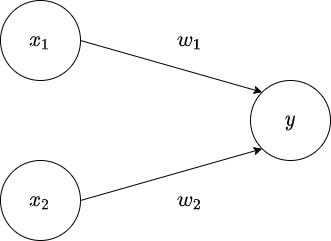
\includegraphics[width=0.50\hsize, keepaspectratio]{images/drawio/pa-seputoron.png}
 \caption{2入力パーセプトロン}
 \label{fig:pa-septoron}
\end{figure}

\subsection{ニューラルネットワーク}

\subsection{DNN (Deep Neural Networks)}

\subsection{CNN (Convolutional Neural Networks)}

\subsection{モデルの過学習}



\newpage
\section{層の説明}
\subsection{全結合層}
\subsection{畳み込み層}
\subsection{プーリング層}
\subsection{ドロップアウト層}

\section{活性化関数}
\subsubsection{sigmoid関数}
\subsubsection{ReLu関数}
\subsubsection{softmax関数}


\section{損失関数と重み更新}
\subsection{損失関数}
深層学習の学習で用いられる指標を,損失関数と呼ぶ.損失関数には様々な種類が存在し,解く問題の種類によって使い分ける.
一般的な損失関数として,式(\ref{eq:mse})の2乗平均誤差(主に回帰問題に使用) や,式(\ref{eq:ce})のクロスエントロピー誤差(主に分類問題に使用)が挙げられる.

\begin{equation}
	E = \frac{1}{n} \sum_{i=1}^{n} (\hat{y_i} - y_i)^2
	\label{eq:mse}
\end{equation}

\begin{equation}
	E = sans
	\label{eq:ce}
\end{equation}

\subsection{最適化手法}


\newpage
\chapter{使用するデータセット}
\section{Sloan Digital Sky Survey(SDSS)}
\subsection*{Sloan Digital Sky Survey (以下,SDSS)について}
SDSS\ref{}とは,天文学史上最も重要なサーベイ観測プロジェクトの一つとも称される大規模プロジェクトである.このプロジェクトは全天の約1/4の天域において,天体の画像および分光データを取得し,天体カタログを作成することを目的としたものである.SDSSでの撮像・分光データ取得はCCDを搭載した地上望遠鏡によって行われる.SDSSの最初のプロジェクトであるSDSS-Iは2000年から2008年まで行われ,また対象を銀河系や超新星に絞ったSDSS-IIが2005年から2008年にSDSS-Iと並行して実施された.その後,太陽系外惑星調査や天の川銀河の構造及び進化などに焦点を当てたSDSS-IIIが2008年から2014年に,南天・北天からの銀河系探索などを目的としたSDSS-IVが2014年から2020年に行われた.

SDSSで撮影された天体のうち低赤方偏移銀河は後述するGalaxy Zooによって形態分類ラベル付けが行われている.SDSSとGalaxy Zooから天体の画像データと分類ラベルを取得できることから,これらのセットを今回の銀河形態分類モデル作成に用いる.
\subsection*{実験に用いる銀河画像データの作成方法}
今回分類モデル学習に用いる銀河画像データとして,SDSS-IIにおけるデータリリースの中から,Data Release 7 (以下,DR7)\ref{}より画像データの取得を行った.DR7 を選んだ理由としては,Galaxy Zooにおける銀河形態ラベル付けにDR7の銀河画像が用いられたからである.

データベースから取得できるのはある程度大きな天域の全体画像のため,用いたい銀河の画像を取得したい場合は,全体画像から切り出しを行う必要がある.今回はGalaxy Zooにて形態ラベル付けが為されている銀河の中から15,000天体を対象に,銀河毎に64ピクセル四方のサイズで切り出しを行った.銀河切り出し画像の生成概略図を図\ref{}に示す.

DR7におけるデータの撮影が行われたSDSS-IIにおいて,銀河撮像に用いられた測光フィルタはu, g, r, i, zの5つが存在し,これらのフィルタを使用し5つの帯域画像が撮影された(図\ref{fig:dr7_filters}参照).これら5つの帯域画像のうち,今回の実験ではrフィルタから得られた帯域画像(rバンド画像)を使用している.rバンド画像を使用した理由としては,5つの帯域画像のうち可視光帯画像であるg, r, iバンド画像の中で,最も平均値に近い波長を捉えているrバンド画像がより多くの銀河形態的特徴を有していると考えられること,またrフィルタが5つの測光フィルタのうち最も感度がよいことが挙げられる\ref{}.

\begin{figure}[H]
	\centering
	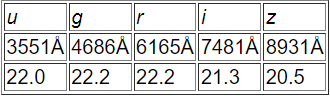
\includegraphics[width=8cm]{images/dr7_filters.png}
	\caption{SDSS Data Release 7 における,銀河撮像に用いられた測光フィルタ一覧\\(フィルタ名,各フィルタによって撮影された画像の波長平均値)}
	\label{fig:dr7_filters}
\end{figure}

\begin{figure}[H]
 \centering
 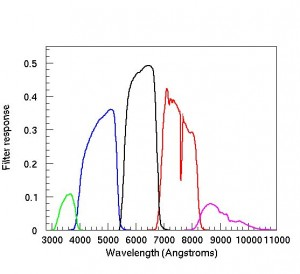
\includegraphics[width=11cm]{images/camera_filters-300x274.png}
 \caption{SDSSにおける測光フィルタのスループット曲線\\(https://www.sdss.org/instruments/camera/ より引用)}
 \label{fig:filter_responces}
\end{figure}



\section{Galaxy Zoo (GZ)}
\subsection*{Galaxy Zoo (以下,GZ)について}
Galaxy Zoo\ref{Lintott2008}とは,人間の目による分類を行い銀河形態カタログを作成したプロジェクトである.従来の銀河形態分類は専門知識を持った天文学者のチームによって行われてきたが,SDSSのような何十万もの銀河が格納されたデータセットが登場するに従い,天文学者だけでは銀河データの増加に追いつけなくなってきた.このような状況を打破する方法として,インターネットを通じて専門知識を持たない有志の一般人に投票形式で形態分類を行わせる方法が提案された.これがGZである.

GZの最初の調査であるGalaxy Zoo 1\ref{Lintott2010}では渦巻銀河か楕円銀河の区別や,渦巻銀河であった場合にどちら周りに渦巻いているかなどを投票形式で集計し,6つのカテゴリへと分類が行われた.GZ1 の後継プロジェクトであるGalaxy Zoo 2\ref{Willett2013}では,GZ1より詳細な形態分類を行うため11つの質問が用意されている.

\subsection*{GZ1における形態ラベル付け方法}
GZ1では,ウェブサイト(www.galaxyzoo.org)を通じて有志の一般人の形態分類を投票形式で集計した.GZ1における分類の投票ページを図\ref{fig:gz1_website}に示す.サイトを訪れた有志の一般人は,楕円銀河・時計回り渦巻銀河・反時計回り渦巻銀河・エッジオン (渦が地球から観測できない向きについている銀河)・星もしくは区別できなかった天体・マージャー (2つの銀河が衝突し合体している,合体銀河)の6つのうちいずれかに投票を行う.形態分類カタログは,対象となった銀河に対し,各形態分類の投票率を付与され作成される.

\begin{figure}[h]
 \centering
 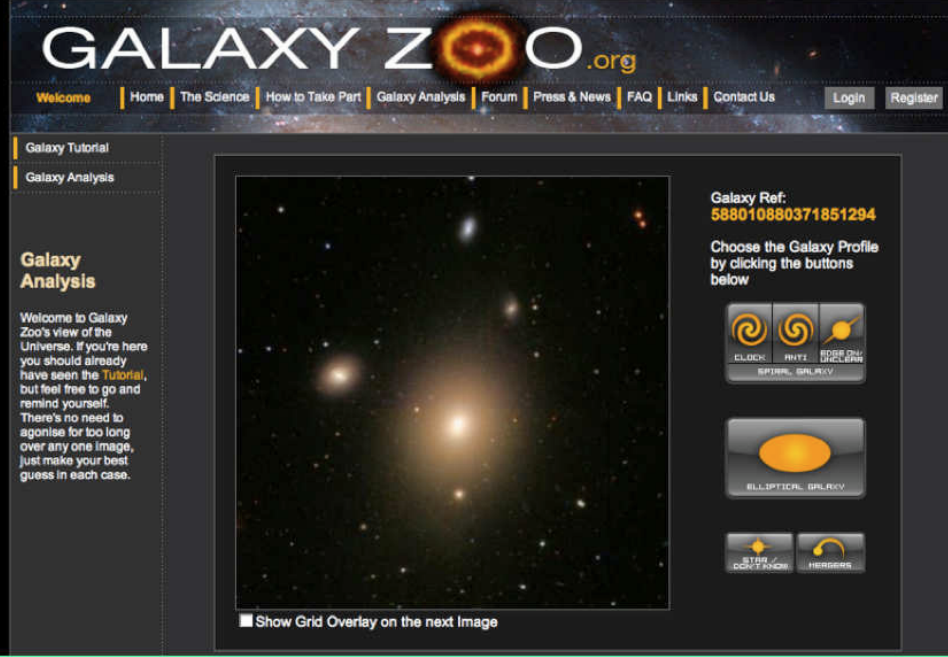
\includegraphics[width=12cm]{images/gz1_website.png}
 \caption{GZ1における形態分類の投票ウェブページ\\(\ref{Lintott2010}より引用)}
 \label{fig:gz1_website}
\end{figure}

\subsection*{実験に用いる正解ラベルの作成方法}
今回分類モデル学習に用いる正解ラベルとして,GZ1から取得できるTable2の分類フラグを用いた.Table2の記載内容を示した図を図\ref{fig:table2}に示す.Table2はSDSSから取得した天体のうち,分光スペクトルデータが観測された天体に関して収録されている.Table2には以下の情報が記載されている.

\begin{quote}
 \begin{itemize}
	\item SDSSにおける天体オブジェクトID
	\item 天体の天球座標 (RA, Dec)
	\item 投票数
	\item 各カテゴリの得票率
	\item バイアスが除去された投票率
	\item 分類フラグ (渦巻銀河・楕円銀河・不確かな天体)
 \end{itemize}
\end{quote}

分類フラグは,渦巻銀河・楕円銀河・不確かな天体の3つが存在する.それぞれの銀河種に対し,得票率が8割を超えた場合にフラグが立つ.今回はこの分類フラグを深層学習モデルの学習に用いる.

\begin{figure}[h]
 \centering
 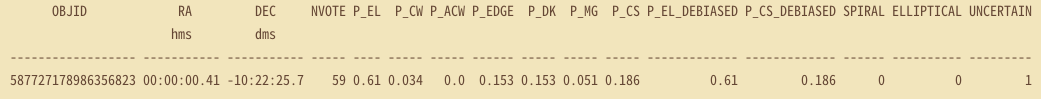
\includegraphics[width=18cm]{images/table2.png}
 \caption{Table2}
 \label{fig:table2}
\end{figure}

\newpage
\chapter{SDSS \& Galaxy Zooを用いた分類モデル学習}
この章では当論文の実験で用いられるSDSSとGZにて,学習データとテストデータの解像度が揃っているという条件のもと,高精度分類が行える分類モデルを学習させることを目的とし,その結果2つの実験を行った.

第4章を行う動機は,当論文で掲げている将来展望の前提条件を達成することである.当論文の将来展望は,高空間分解能観測装置データを用いてモデル学習を行うことで,既存の低空間分解能データセットに対し更なる高精度形態分類を提供するというものである.この将来展望にまつわる実験の最も初段階の前提条件として,まずは学習データとテストデータの解像度が揃っている条件にて高精度分類が行えるかを検証する必要がある.そこで2つの実験を行った.

\section{実験概要}
第4章ではSDSSから取得した銀河画像とGZから取得した分類フラグを学習データとし,渦巻銀河・楕円銀河・不確かな天体のいずれかを予測する分類モデルを学習する.
\subsubsection{学習データ}
学習に用いる画像データは,SDSSから取得した64ピクセル四辺の銀河切り出し画像を使用し,正解ラベルはGZから取得した分類フラグを用いる.実験には15,000天体を用いた.15,000天体の赤方偏移別の個数を示したグラフを図\ref{fig:z_15000}に示す.一般的に赤方偏移の値が小さいほど,地球から近い天体といえる.15,000天体のうち,GZの分類フラグにて渦巻銀河と分類されている天体は4,058天体,楕円銀河は1,561天体,不確かな天体は9,310天体であった.渦巻銀河・楕円銀河・不確かな天体の切り出し画像の例を図\ref{}から図\ref{}に示す.

モデルの学習および評価の際,モデルの学習データとテストデータの比率は7:3とした.

\begin{figure}[h]
 \centering
 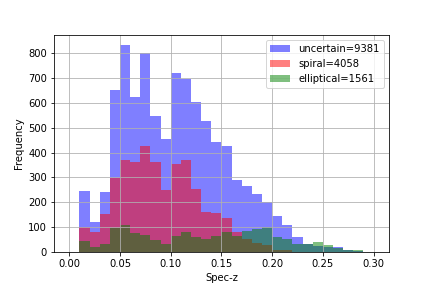
\includegraphics[width=14cm]{images/z_15000_4.png}
 \caption{実験に用いる15,000天体の赤方偏移別の個数グラフ}
 \label{fig:z_15000}
\end{figure}

\newpage
\begin{figure}[H]
 \centering
 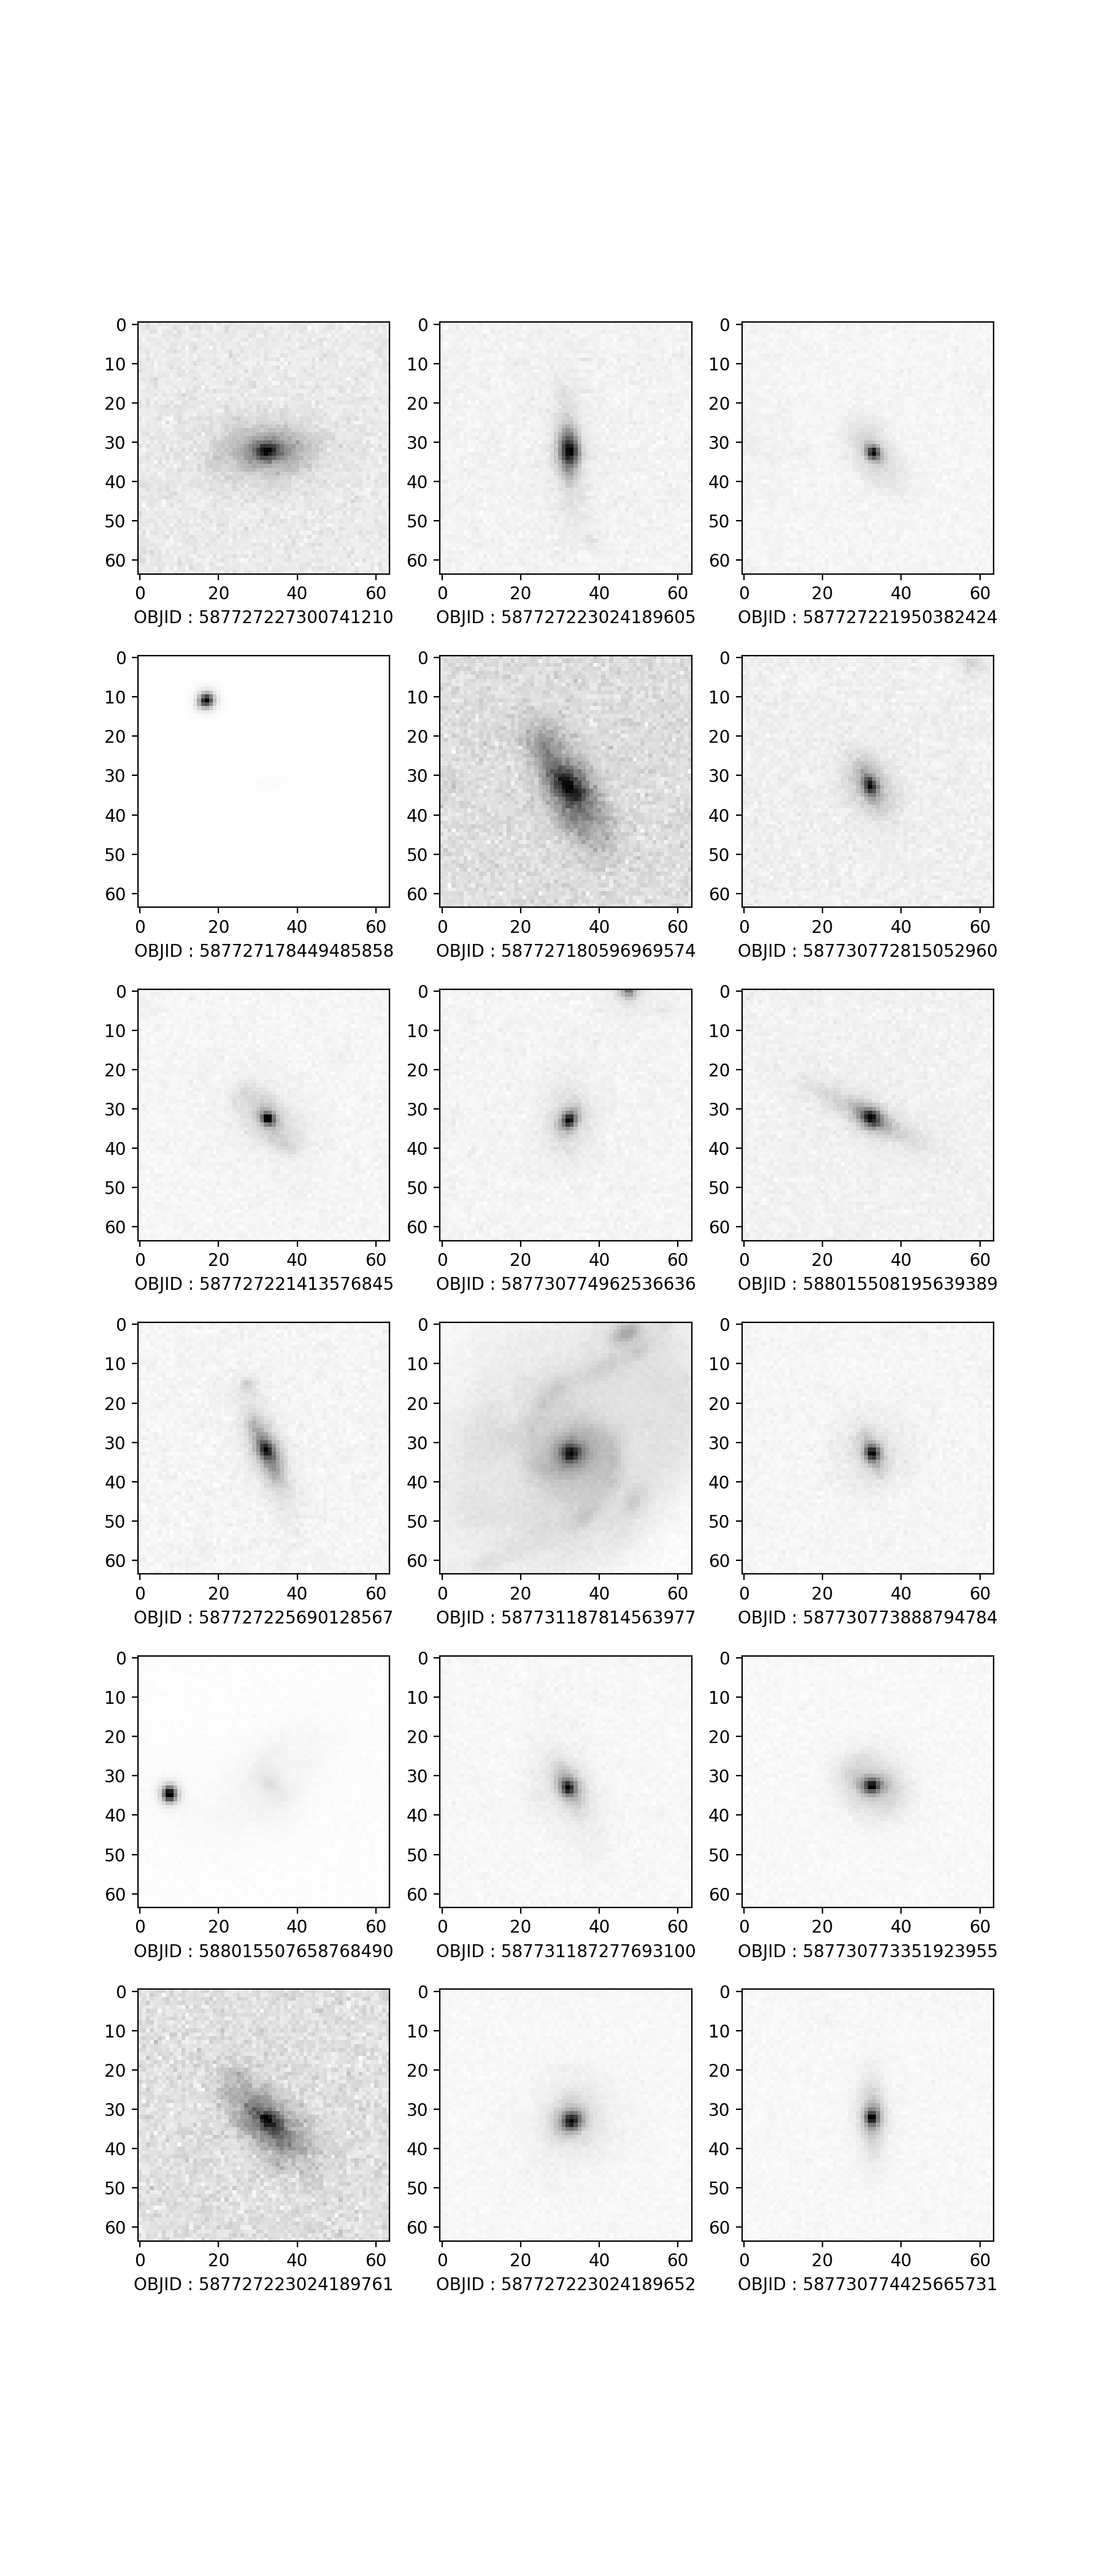
\includegraphics[width=0.6\vsize, keepaspectratio]{images/syuron_4syou_sdss_imgs/spiral.png}
 \caption{渦巻銀河の切り出し画像の例}
 \label{fig:sdss_images_spiral}
\end{figure}

\newpage
\begin{figure}[H]
  \centering
  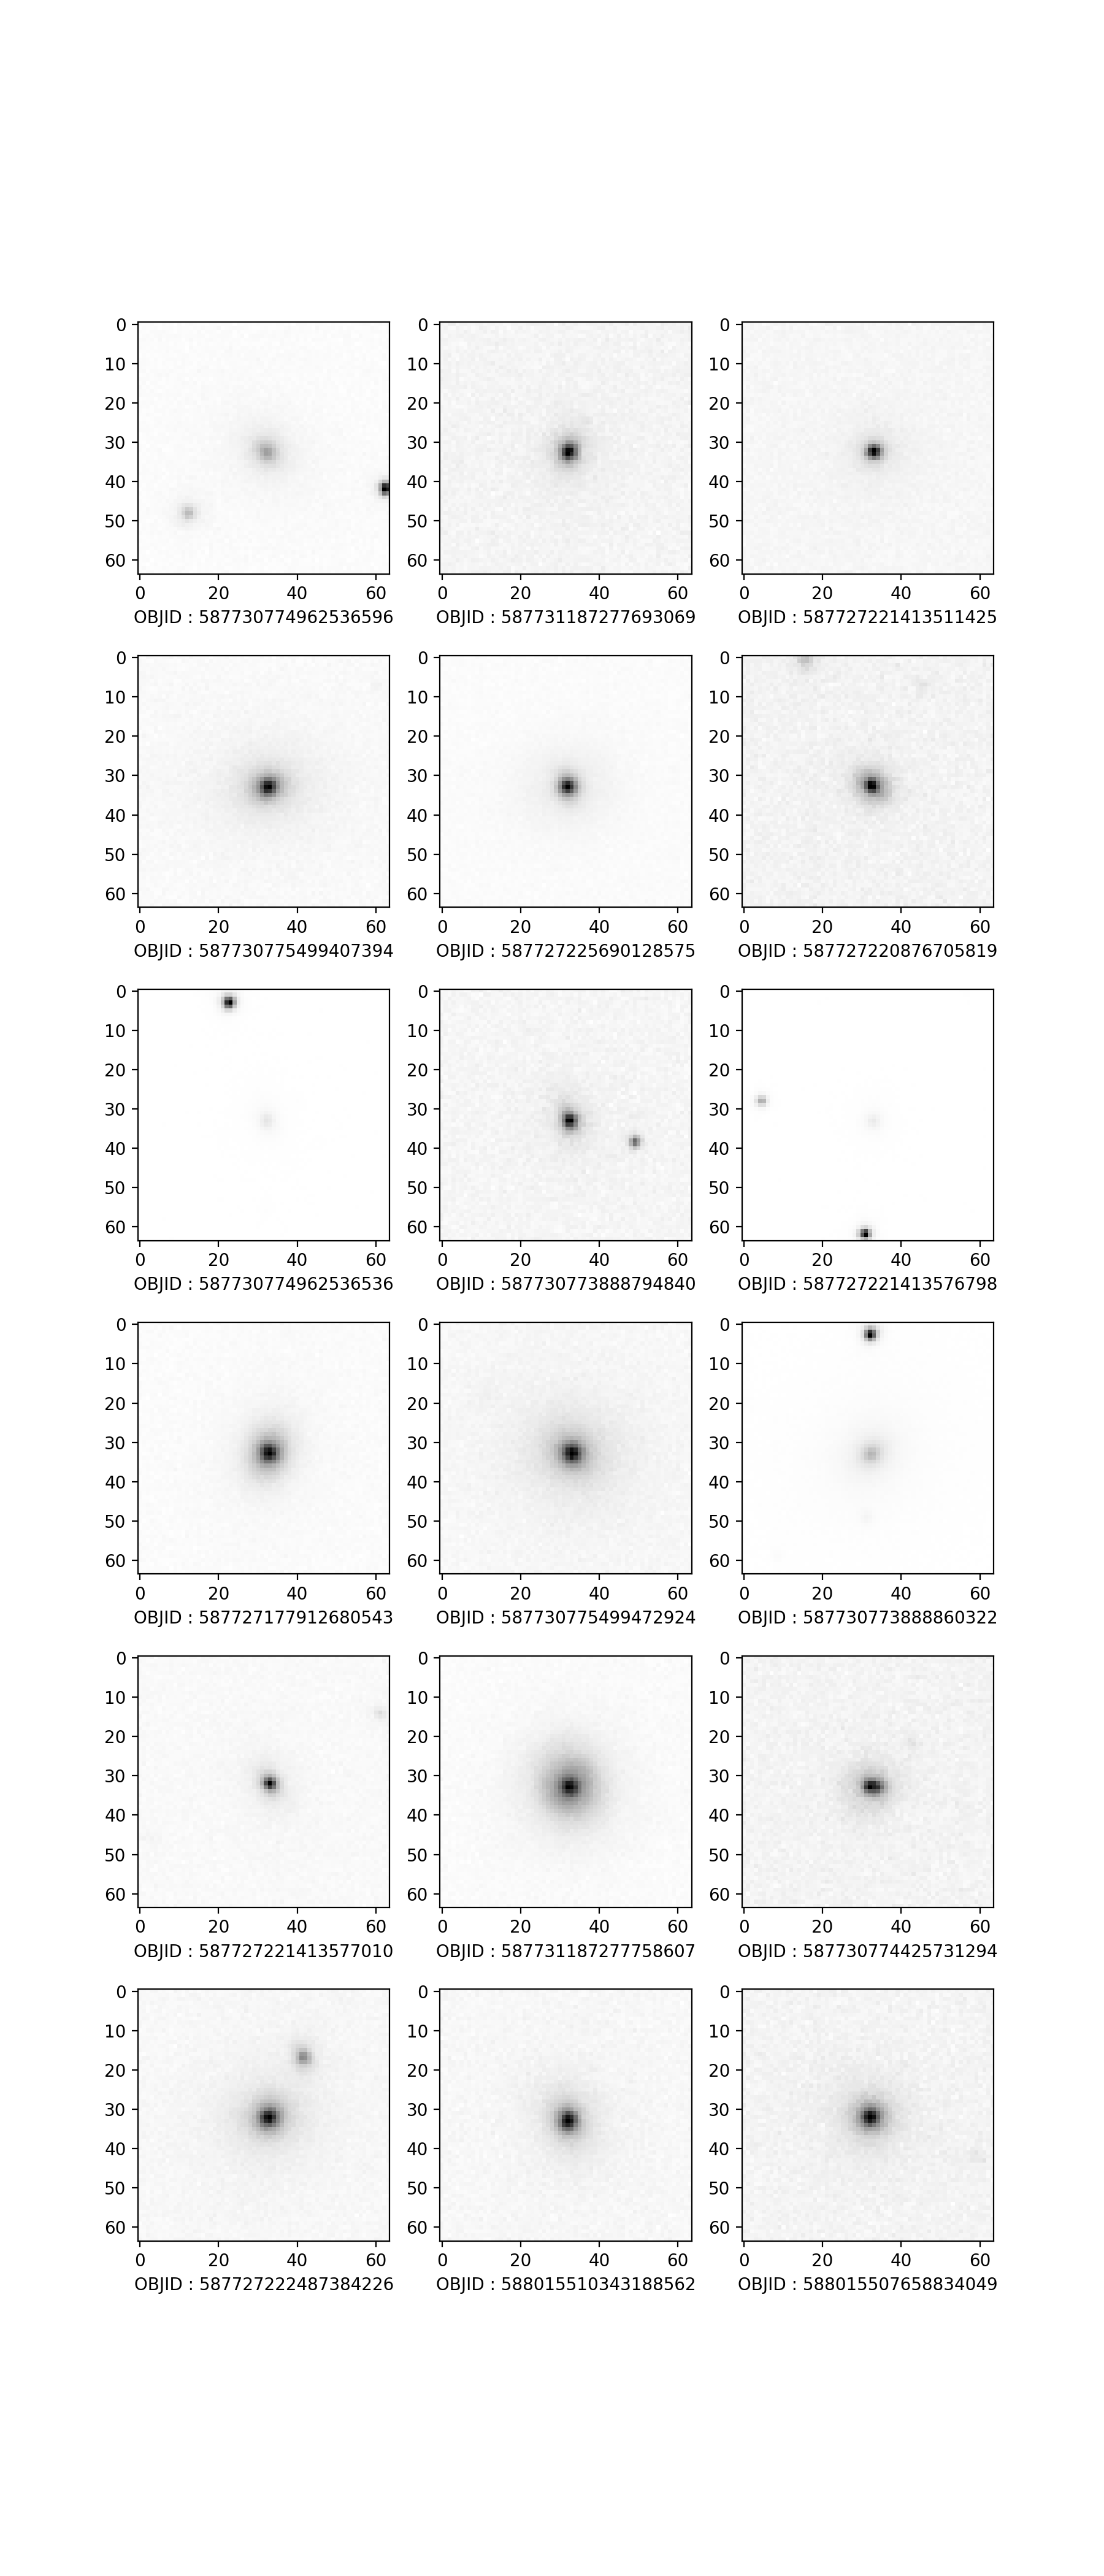
\includegraphics[width=0.6\vsize, keepaspectratio]{images/syuron_4syou_sdss_imgs/elliptical.png}
  \caption{楕円銀河の切り出し画像の例}
  \label{fig:sdss_images_elliptical}
\end{figure}

\subsubsection{モデル構造}
今回用いた深層学習モデルは,cheng et al.(2019)\ref{Cheng2019}にて用いられていた銀河形態分類モデルを参考にした.今回用いたモデルの構造を図\ref{fig:model_shape}に示す.このモデルは畳み込み層を合計3つ有しており,それぞれのカーネルサイズは3x3, 3x3, 2x2である.それぞれの畳み込み層の後には,2x2のmax-pooling層が存在する.全畳み込み層の後に全結合層が2層配置されており,それぞれ1024個のノードを有している.

\begin{figure}[h]
	\centering
	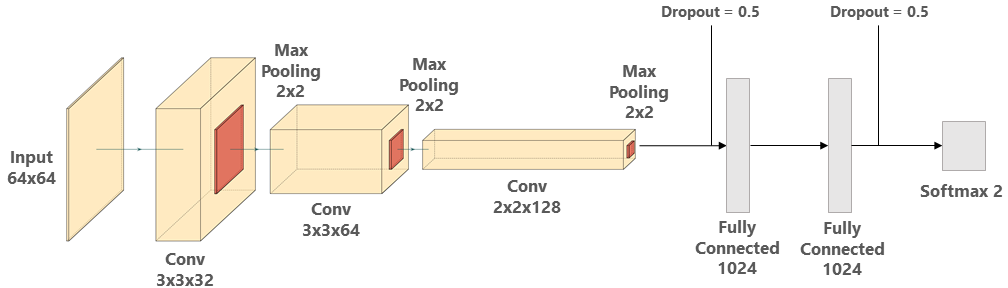
\includegraphics[width=14cm]{images/model_shape.png}
	\caption{用いた分類モデルの構造図}
	\label{fig:model_shape}
\end{figure}
 
\subsubsection{モデルの評価方法}
分類モデルの評価指標として,主にaccuracy (正解率)とtrue positive rate (真陽性率),そして一部実験においてTrue Skill Statistics (以下,TSS)を用いた.accuracyは全テストデータの中で正しく分類できたデータがどれだけあるかというものであり,モデルの正確性を表す指標である.true positive rateは本来陽性だと分類すべき全データのうち,どれほど正しく分類できたかを表す指標である.TSSもaccuracyと同じく正確性を表す指標であるが,テストデータ内のデータインバランス性に対しロバストな性質がある.

以下に2値分類問題を例とした場合の混同行列,accuracy, true positive rateおよびTSSの導出方法を示す.ここで混同行列とは,分類問題においてモデルが予測した値および真の値を行列形式で表したものであり,分類モデルの性能を可視化・評価するのによく用いられる指標である.モデルの予測値と真の値が交差する対角成分における数が多いほど,モデルが正確な予測を行っているといえる.

\begin{figure}[H]
 \centering
 
\includegraphics[width=12cm]{images/cm.png}
 \caption{2値分類問題における混同行列}
 \label{fig:cm}
\end{figure}

\begin{equation}
 accuracy = \frac{TP + TN}{TP + FP + FN + TN}
 \label{equ:accuracy}
\end{equation}

\begin{equation}
 true positive rate = \frac{TP}{TP + FN}
 \label{}
\end{equation}

\begin{equation}
	TSS = \frac{TP}{TP + FN} - \frac{FP}{TN + FP}
 \label{equ:tss}
\end{equation}

また,深層学習モデルには実行毎に学習のブレが存在するため,モデルの評価の際には学習・テストを30回実行し,評価指標の平均値,標準偏差および標準誤差を導出する.

\section{不確かラベルが与える分類精度への影響}
GZが与える形態分類フラグのうち「不確かな天体」というフラグが立っている天体は,渦巻銀河・楕円銀河のどちらの得票率も8割を超えなかった天体である.これらの天体は人間の目による形態分類が比較的難しい天体,つまり天体画像から読み取れる形態的特徴があいまいな天体であると考えられる.

この節では特徴があいまいだと考えられる不確かな天体群が,形態分類モデルの分類精度に与える影響を調べる.具体的には以下の2条件でモデルの学習・テストを行い,テストデータに対する予測のaccuracyや混同行列の比較をする.そして不確かな天体の特性や学習に用いた際に分類精度に与える影響を調べる.
\begin{quote}
 \begin{itemize}
	\item 不確かを含めた,渦巻・楕円・不確かの3値分類
	\item 不確かを除いた,渦巻・楕円の2値分類
 \end{itemize}
\end{quote}

\subsection{実験条件}
モデルの学習およびテストを行う天体数は1,000天体とした.使用する天体は,GZによる形態分類が行われた15,000天体(図\ref{fig:z_15000}参照)からランダムに取得を行う.取得を行う際,赤方偏移$z$について,$0 < z < 0.2$という条件を設定し,あてはまらない天体は除外を行う.これは,地球との距離が遠すぎる天体については上手く特徴抽出が行えず学習の妨げになる可能性があるからである.

使用天体を1,000天体取得したあと,学習データとテストデータの比率が7:3となるように切り分けを行った.

モデルの評価を行う際,モデルの学習およびテストを30回行い,accuracyの平均値,標準偏差および標準誤差を導出した.なお,30回の学習およびテストの際,学習実行毎に取得される天体は毎回シャッフルされる.

\subsection{実験結果}
\subsubsection{学習結果}
不確かを含めた渦巻・楕円・不確かの3値分類モデル,および不確かを除いた渦巻・楕円の2値分類モデルの学習結果を図\ref{fig:losses_ex4-1}から図\ref{fig:cm_ex4-2}に示す.

\begin{quote}
 \begin{itemize}
	\item 一番上の図は,横軸epoch数・縦軸loss(損失関数)となっている.
	\item 中段の図は,横軸epoch数・縦軸accuracy(正解率)となっている.
	\begin{quote}
	 \begin{itemize}
		\item これら2つの図は,青色のラインが学習データに対するスコア,黄色のラインがテストデータに対するスコアとなっている.
		\item lossのグラフについて,学習データに対する損失関数は学習が進むにつれ順当に下がっていくものの,ある一定のepochからテストデータに対する損失関数が上昇していく現象が見受けられる.この現象は\textbf{過学習}と呼ばれている.この現象が起こると,学習データに対し分類モデルが過剰に適合した結果,学習データに対する予測精度に比べテストデータに対する予測精度が低下していく.
	 \end{itemize}
	\end{quote}
	\item 一番下の図はテストデータに対する予測結果から生成した混同行列であり,行成分がモデルによる予測ラベル,列成分がテストデータの真のラベルである.
 \end{itemize}
\end{quote}

\begin{figure}[htbp]
  \begin{minipage}[b]{0.45\hsize}
    \centering
    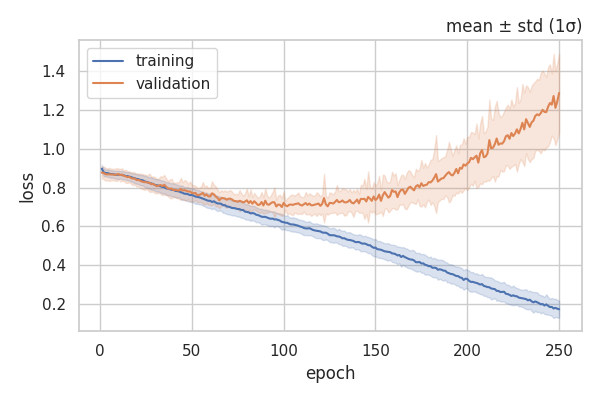
\includegraphics[keepaspectratio, width=7cm]{images/losses_ex4-1.png}
    \caption{3値分類 : loss関数の学習遷移}
		\label{fig:losses_ex4-1}
  \end{minipage}
  \begin{minipage}[b]{0.45\hsize}
    \centering
    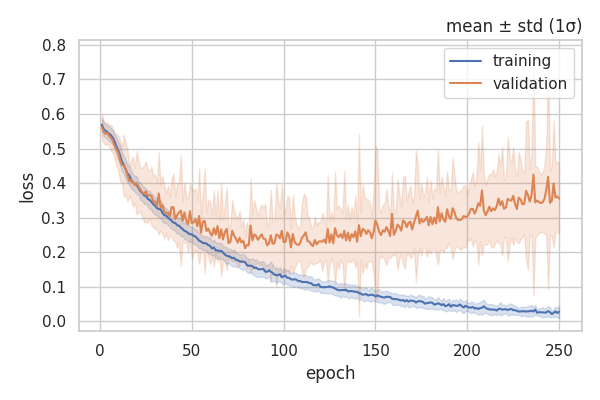
\includegraphics[keepaspectratio, width=7cm]{images/losses_ex4-2.png}
    \caption{2値分類 : loss関数の学習遷移}
		\label{fig:losses_ex4-2}
  \end{minipage}
\end{figure}

\begin{figure}[htbp]
  \begin{minipage}[b]{0.45\hsize}
    \centering
    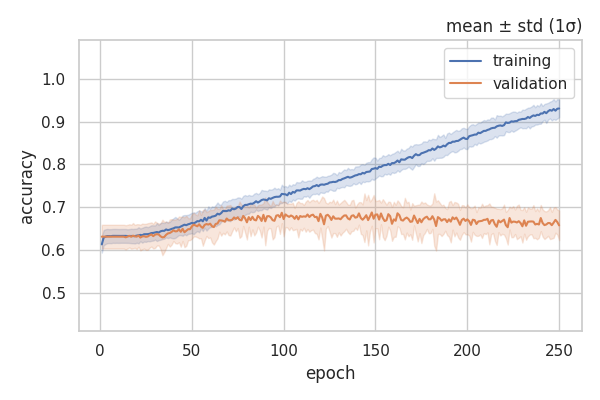
\includegraphics[keepaspectratio, width=7cm]{images/accs_ex4-1.png}
    \caption{3値分類 : accuracyの学習遷移}
		\label{fig:accs_ex4-1}
  \end{minipage}
  \begin{minipage}[b]{0.45\hsize}
    \centering
    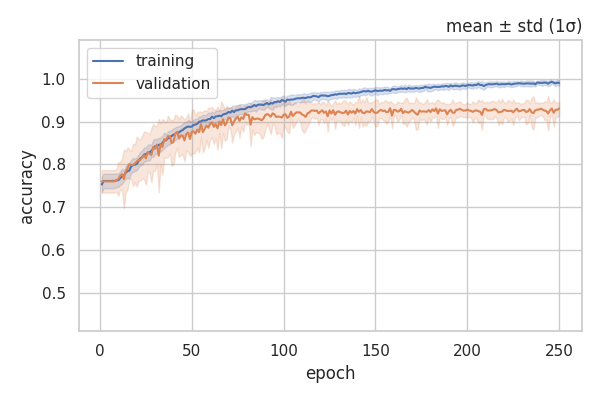
\includegraphics[keepaspectratio, width=7cm]{images/accs_ex4-2.png}
    \caption{2値分類 : accuracyの学習遷移}
		\label{fig:accs_ex4-2}
  \end{minipage}
\end{figure}

\newpage

\begin{figure}[H]
  \begin{minipage}[b]{0.45\hsize}
    \centering
    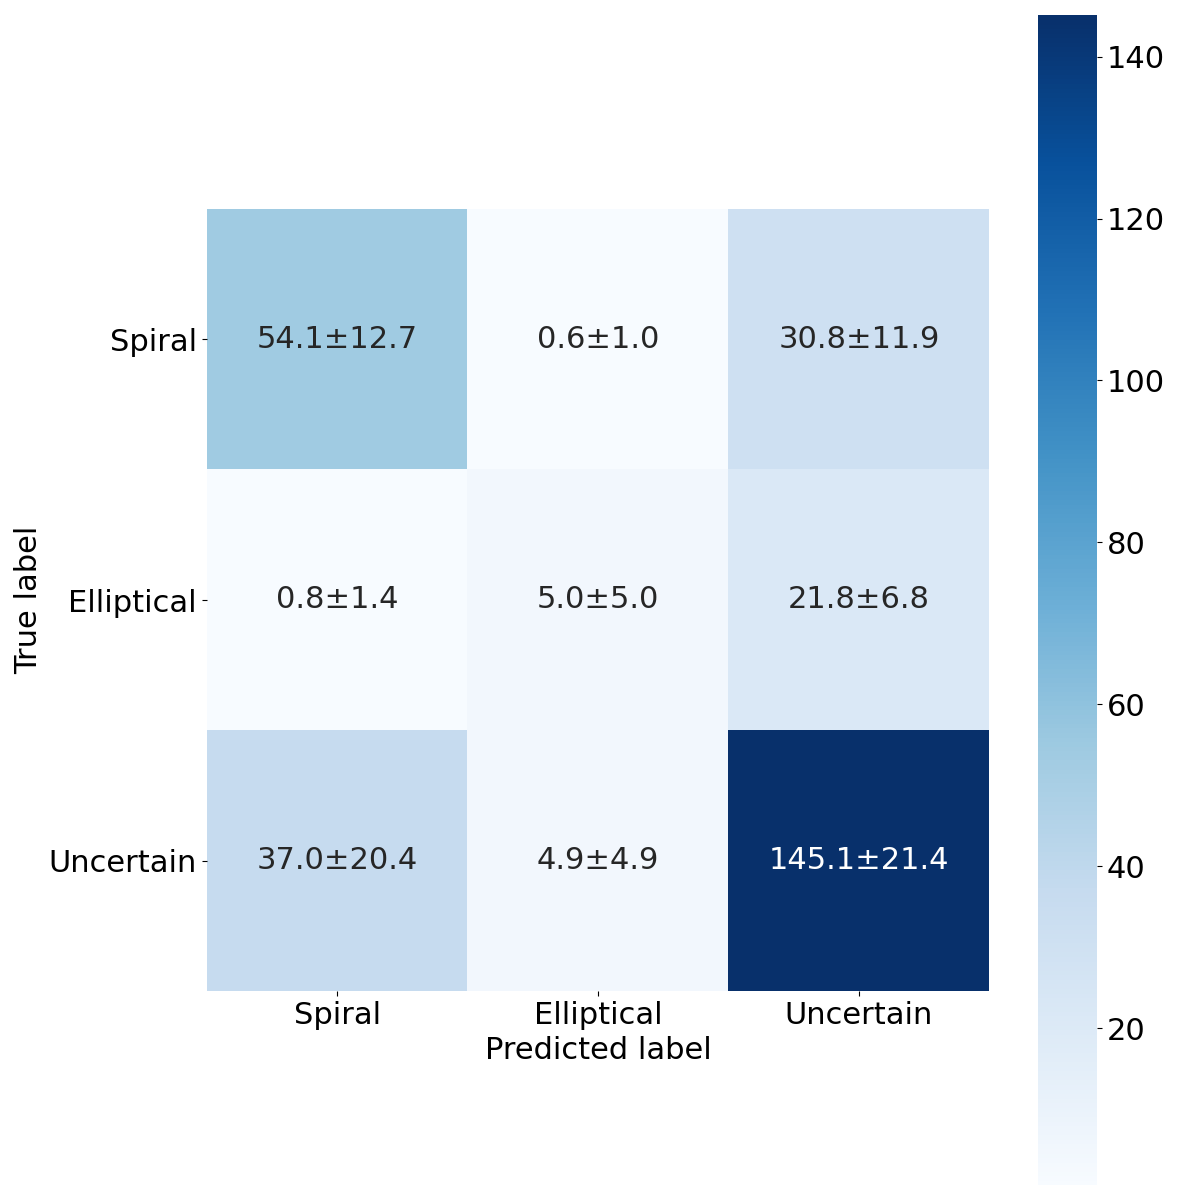
\includegraphics[keepaspectratio, width=7cm]{images/cm_mean_std_ex4-1.png}
    \caption{3値分類 : 混同行列\\(平均$\pm$標準偏差(1$\sigma$))}
		\label{fig:cm_ex4-1}
  \end{minipage}
  \begin{minipage}[b]{0.45\hsize}
    \centering
    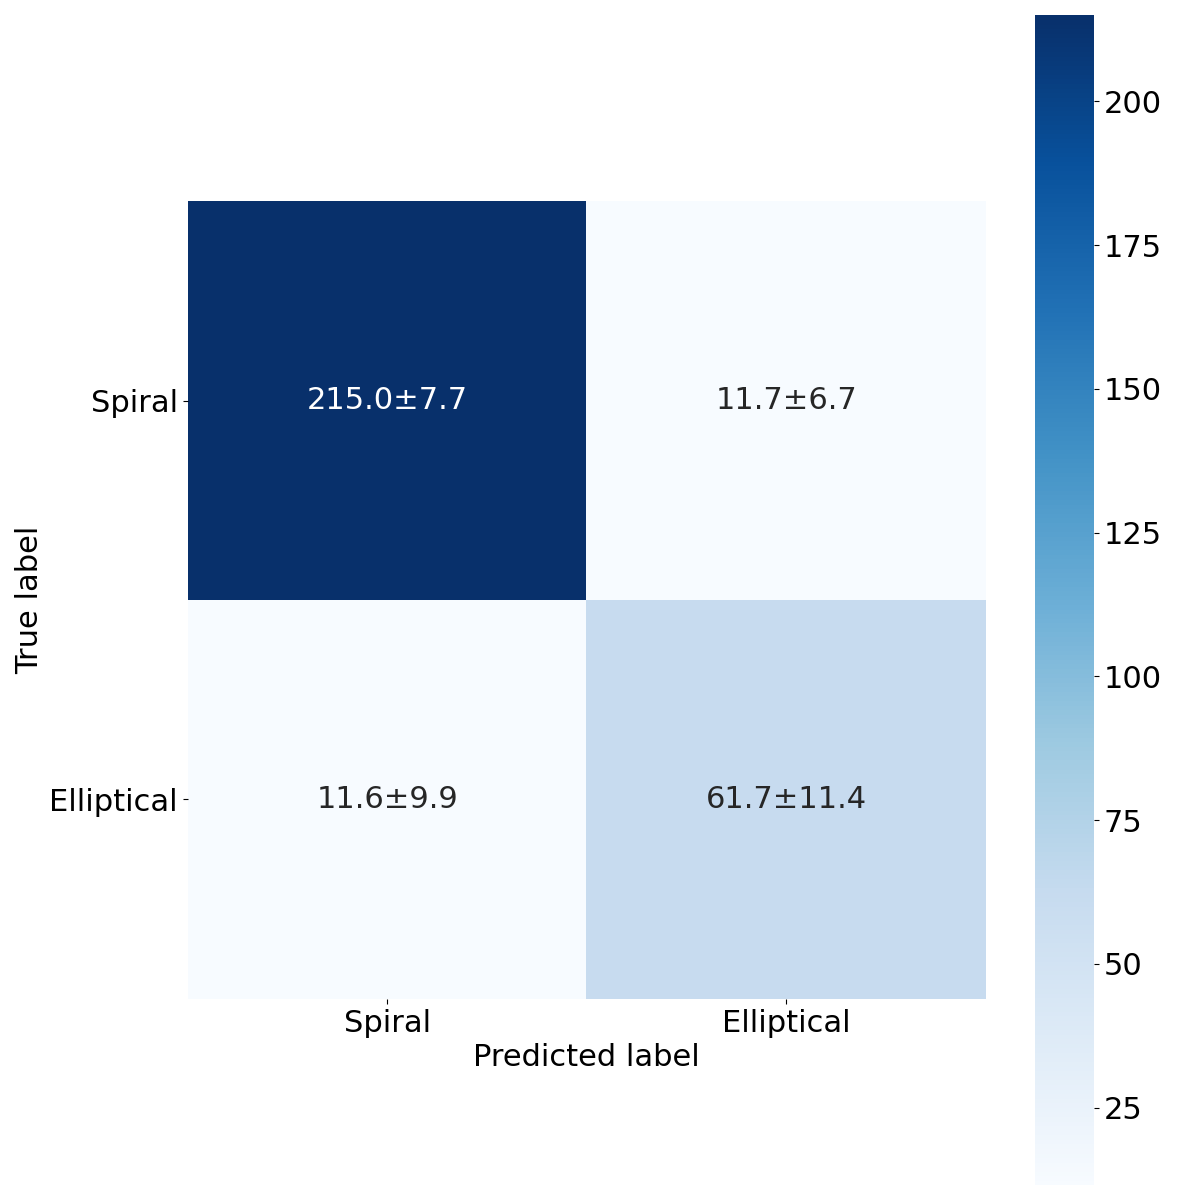
\includegraphics[keepaspectratio, width=7cm]{images/cm_mean_std_ex4-2.png}
    \caption{2値分類 : 混同行列\\(平均$\pm$標準偏差(1$\sigma$))}
		\label{fig:cm_ex4-2}
  \end{minipage}
\end{figure}

\subsubsection{結果}
\paragraph{モデル学習の進行}
図\ref{fig:losses_ex4-1}・図\ref{fig:accs_ex4-1}において,テストデータに対するスコアが100epoch付近までloss関数は降下,accuracyは上昇し,それ以降のepochではloss関数が上昇,accuracyが降下していることから,3値分類モデルでは100epochまで学習が良い方向に進んでいるもののそれ以降のepochからはモデルが学習データに対し過学習し,テストデータに対する汎化性能を失っていることが分かる.

また図\ref{fig:losses_ex4-2}・図\ref{fig:accs_ex4-2}において,テストデータに対するスコアが100epoch付近までloss関数は降下,accuracyは上昇するものの,それ以降のepochではloss関数は上昇するがaccuracyは横ばいになっている.このことから,2値分類モデルにおいては100epoch目以降学習データに対し過適合はしているものの,テストデータに対する汎化性能は失っていないことが読み取れる.

\paragraph{テストデータに対するaccuracyの評価}
モデルの形態分類性能を評価するため,両モデル間にてテストデータに対するaccuracyの比較を行う.性能評価においては,モデルが学習しきった際の分類性能を用いる.すなわち,accuracyを採るepoch数は,テストデータに対するaccuracyが最大となるepoch数とした.


不確かを含めた渦巻・楕円・不確かの3値分類モデル,および不確かを除いた渦巻・楕円の2値分類モデルにおける,テストデータへの予測精度(accuracy)を表\ref{tb:accs_4.2}に示す.3値分類・2値分類ともに,accuracyを採るepoch数を表内に示している.表\ref{tb:accs_4.2}において,1行目には今回の30回実行におけるaccuracyの平均値と標準偏差,2行目にはaccuracyの平均値と今回の30回実行から推定した標準誤差をそれぞれ2$\sigma$分記載した.

表\ref{tb:accs_4.2}より,標準誤差付き平均値において3値分類モデルと2値分類モデルとの間に有意な差があり,なおかつ2値分類モデルの方がaccuracyが高いことが分かる.また標準偏差付き平均値においても3値分類モデルと2値分類モデルとの間に有意な差があることから,両モデルとも学習のブレがさほど大きくないことが分かる.

\begin{table}[htbp]
  \centering
	\caption{不確か天体を含めた3値分類,および不確か天体を除いた2値分類モデルのテストデータに対する予測のaccuracy}
  \begin{tabular}{|c|c|c|}
		\hline
    & mean$\pm$std (2$\sigma$) & mean$\pm$ste (2$\sigma$) \\ \hline
    3値分類(渦巻・楕円・不確か) & $0.688 \pm 0.062$(148th epoch) & $0.688 \pm 0.011$(148th epoch) \\ \hline
    2値分類(渦巻・楕円) & $0.931 \pm 0.034$(158th epoch) & $0.931 \pm 0.006$(158th epoch) \\ \hline
  \end{tabular}
  \label{tb:accs_4.2}
\end{table}

\paragraph{混同行列の導出方法,および両モデルにおける比較}
混同行列を導出するため,先ほど求めた「モデルが学習しきった地点と思われる,テストデータに対するaccuracyが最大となるepoch数」まで,再度30回学習およびテストを3値分類モデル・2値分類モデル両方にて行った.導出された混同行列をそれぞれ図\ref{fig:cm_ex4-1},図\ref{fig:cm_ex4-2}に示す.図にはそれぞれ個数の平均値と標準偏差が1$\sigma$で示されている.

図\ref{fig:cm_ex4-1}より,3値分類モデルにおいて陽性を不確かな天体とした場合のtrue positive rateは約75\%だが,渦巻銀河群においては約60\%,楕円銀河群においては約20\%である.このことから,学習した3値分類モデルは不確かな天体群に比べ渦巻・楕円銀河を正しく分類する性能が劣っており,特に楕円銀河を正しく分類性能することができないことが読み取れる.
図\ref{fig:cm_ex4-2}より,2値分類モデルにおいて陽性を渦巻銀河とした場合のtrue positive rateは約90\%,楕円銀河とした場合は約80\%であることが分かる.このことから,学習した2値分類モデルにおいて渦巻・楕円銀河を正しく分類する性能は3値分類モデルよりも優れていることが分かる.

また,図\ref{fig:cm_ex4-1},図\ref{fig:cm_ex4-2}より,3値分類モデルに用いたテストデータ内には不確かな天体群が約2/3存在し,また2値分類モデルに用いたテストデータ内には渦巻銀河と楕円銀河の比率がおおよそ3:1となっていることがわかる.これは今回用いる天体の母集団である15,000天体(図\ref{fig:z_15000}参照)の特性と一致している.

\section{データインバランスが与える分類精度への影響}
4.2節において,用いる銀河種を渦巻銀河・楕円銀河の2値とすることで,分類モデルの精度向上が行えることがわかった.一方,図\ref{fig:cm_ex4-1},\ref{fig:cm_ex4-2}より,テストデータにおいて銀河種のデータインバランスが起きていることがわかった.このインバランス性は今回のモデル学習・テストに用いている銀河の母集団(図\ref{fig:z_15000}参照)の性質と一致する.

この節では,学習データ・テストデータ内の銀河種におけるデータインバランス性が,形態分類モデルの分類精度に与える影響を調べる.
具体的には以下の2条件でモデルの学習・テストを行い,テストデータに対する予測のaccuracy,TSSや混同行列の比較をする.そしてデータインバランス性が分類精度に与える影響を調べる.

\begin{quote}
 \begin{itemize}
	\item 渦巻銀河・楕円銀河の比率が異なるインバランスドデータで学習・テストを行った2値分類モデル
	\item 渦巻銀河・楕円銀河の比率が等しいバランスドデータで学習・テストを行った2値分類モデル
 \end{itemize}
\end{quote}

\subsection{実験条件}
モデルの学習およびテストを行う天体の選定方法として,インバランスドデータにおいてはGZによる形態分類が行われた15,000天体(図\ref{fig:z_15000}参照)のうち不確かな天体を除いた渦巻銀河・楕円銀河からランダムに1,000天体の取得を行った.またバランスドデータにおいては渦巻銀河と楕円銀河の比率を等しくするために,15,000天体の母集団のうち不確かな天体を除いた渦巻銀河・楕円銀河から,渦巻銀河を500天体,楕円銀河を500天体取得した.なお取得を行う際,赤方偏移$z$について,$0 < z < 0.2$という条件を設定し,あてはまらない天体は除外を行う.これは,地球との距離が遠すぎる天体については上手く特徴抽出が行えず学習の妨げになる可能性があるからである.

使用天体を1,000天体取得したあと,学習データとテストデータの比率が7:3となるように切り分けを行った.このうちバランスドデータでは,学習データ・テストデータのどちらも渦巻銀河と楕円銀河の比率が等しくなるように1,000天体からの切り分けを行った.

モデルの評価を行う際,モデルの学習およびテストを30回行い,accuracyの平均値,標準偏差および標準誤差を導出した.
なお,30回の学習およびテストの際,学習実行毎に使用される天体は毎回シャッフルされる.
また4.3節の実験においては,モデルの評価指標としてTSSの導出も行った.これはインバランスドデータでのモデル学習・テストにおいて,30回実行における実行毎に取得する天体の渦巻銀河・楕円銀河の比率が毎回異なることから,accuracyだけでは銀河種のデータインバランス性のみを正しく評価できないためである.そこでデータセット内の分類ラベルのインバランス性にロバストな性質をもつTSSも評価指標に加えている.

\subsection{実験結果}
\subsubsection{学習結果}
渦巻銀河・楕円銀河の比率が異なるインバランスドデータで学習を行った2値分類モデル,および渦巻銀河・楕円銀河の比率が等しいバランスドデータで学習を行った2値分類モデルの学習結果を図\ref{fig:losses_ex4-2-2}から図\ref{fig:cm_ex4-3}に示す.

\begin{quote}
	\begin{itemize}
	 \item 一番上の図は,横軸epoch数・縦軸loss(損失関数)となっている.
	 \item 中段の図は,横軸epoch数・縦軸accuracy(正解率)となっている.
	 \begin{quote}
		\begin{itemize}
		 \item これら2つの図は,青色のラインが学習データに対するスコア,黄色のラインがテストデータに対するスコアとなっている.
		 \item lossのグラフについて,学習データに対する損失関数は学習が進むにつれ順当に下がっていくものの,ある一定のepochからテストデータに対する損失関数が上昇していく現象が見受けられる.この現象は\textbf{過学習}と呼ばれている.この現象が起こると,学習データに対し分類モデルが過剰に適合した結果,学習データに対する予測精度に比べテストデータに対する予測精度が低下していく.
		\end{itemize}
	 \end{quote}
	 \item 一番下の図はテストデータに対する予測結果から生成した混同行列であり,行成分がモデルによる予測ラベル,列成分がテストデータの真のラベルである.
	\end{itemize}
 \end{quote}

\begin{figure}[htbp]
  \begin{minipage}[b]{0.45\hsize}
    \centering
    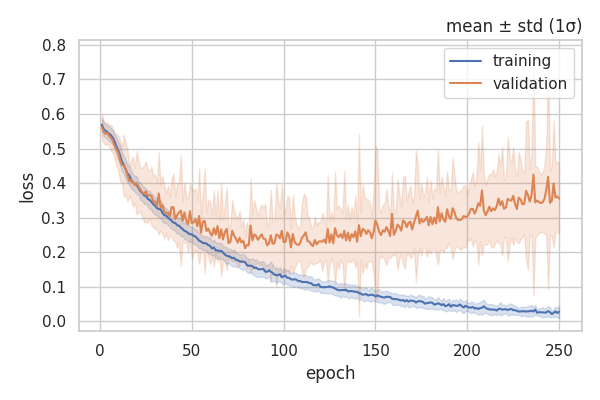
\includegraphics[keepaspectratio, width=7cm]{images/losses_ex4-2.png}
    \caption{インバランスドデータ : loss関数の学習遷移}
		\label{fig:losses_ex4-2-2}
  \end{minipage}
  \begin{minipage}[b]{0.45\hsize}
    \centering
    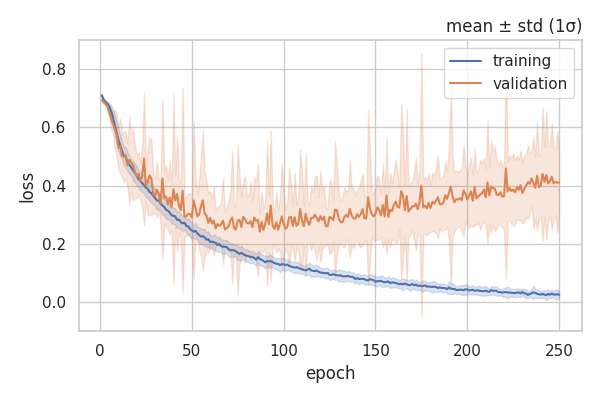
\includegraphics[keepaspectratio, width=7cm]{images/losses_ex4-3.png}
    \caption{バランスドデータ : loss関数の学習遷移}
		\label{fig:losses_ex4-3}
  \end{minipage}
\end{figure}

\begin{figure}[htbp]
  \begin{minipage}[b]{0.45\hsize}
    \centering
    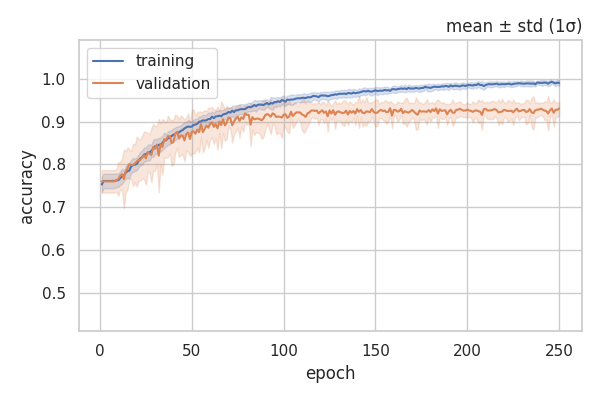
\includegraphics[keepaspectratio, width=7cm]{images/accs_ex4-2.png}
    \caption{インバランスドデータ : accuracyの学習遷移}
		\label{fig:accs_ex4-2-2}
  \end{minipage}
  \begin{minipage}[b]{0.45\hsize}
    \centering
    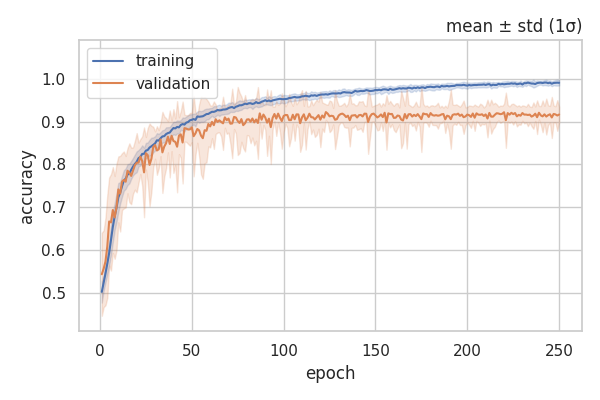
\includegraphics[keepaspectratio, width=7cm]{images/accs_ex4-3.png}
    \caption{バランスドデータ : accuracyの学習遷移}
		\label{fig:accs_ex4-3}
  \end{minipage}
\end{figure}

\newpage

\begin{figure}[H]
  \begin{minipage}[b]{0.45\hsize}
    \centering
    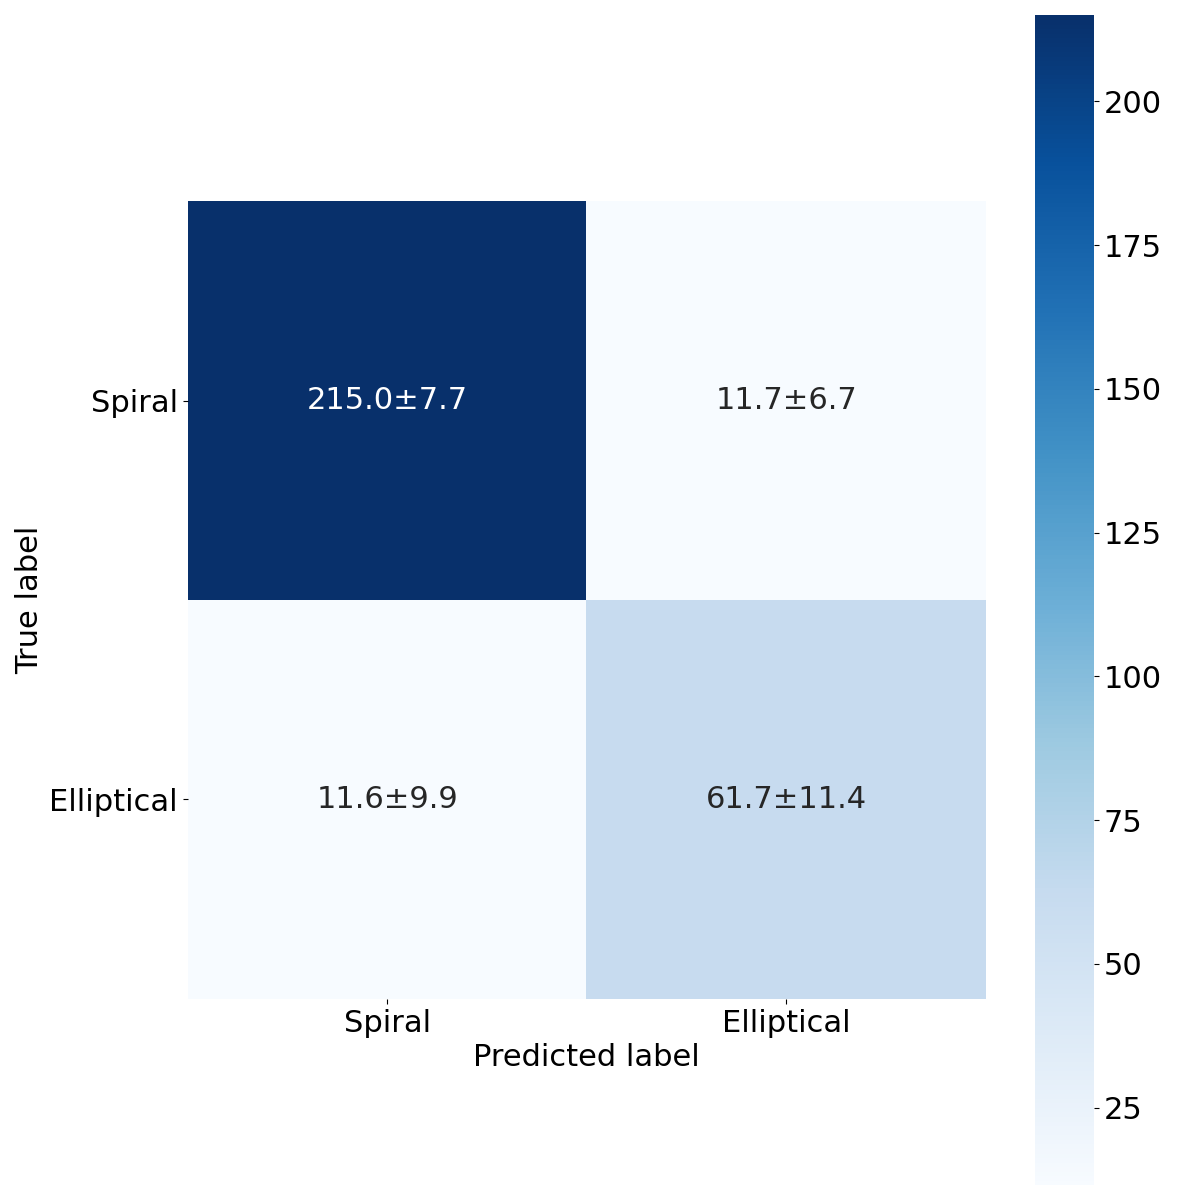
\includegraphics[keepaspectratio, width=7cm]{images/cm_mean_std_ex4-2.png}
    \caption{インバランスドデータ : 混同行列\\(平均$\pm$標準偏差(1$\sigma$))}
		\label{fig:cm_ex4-2-2}
  \end{minipage}
  \begin{minipage}[b]{0.45\hsize}
    \centering
    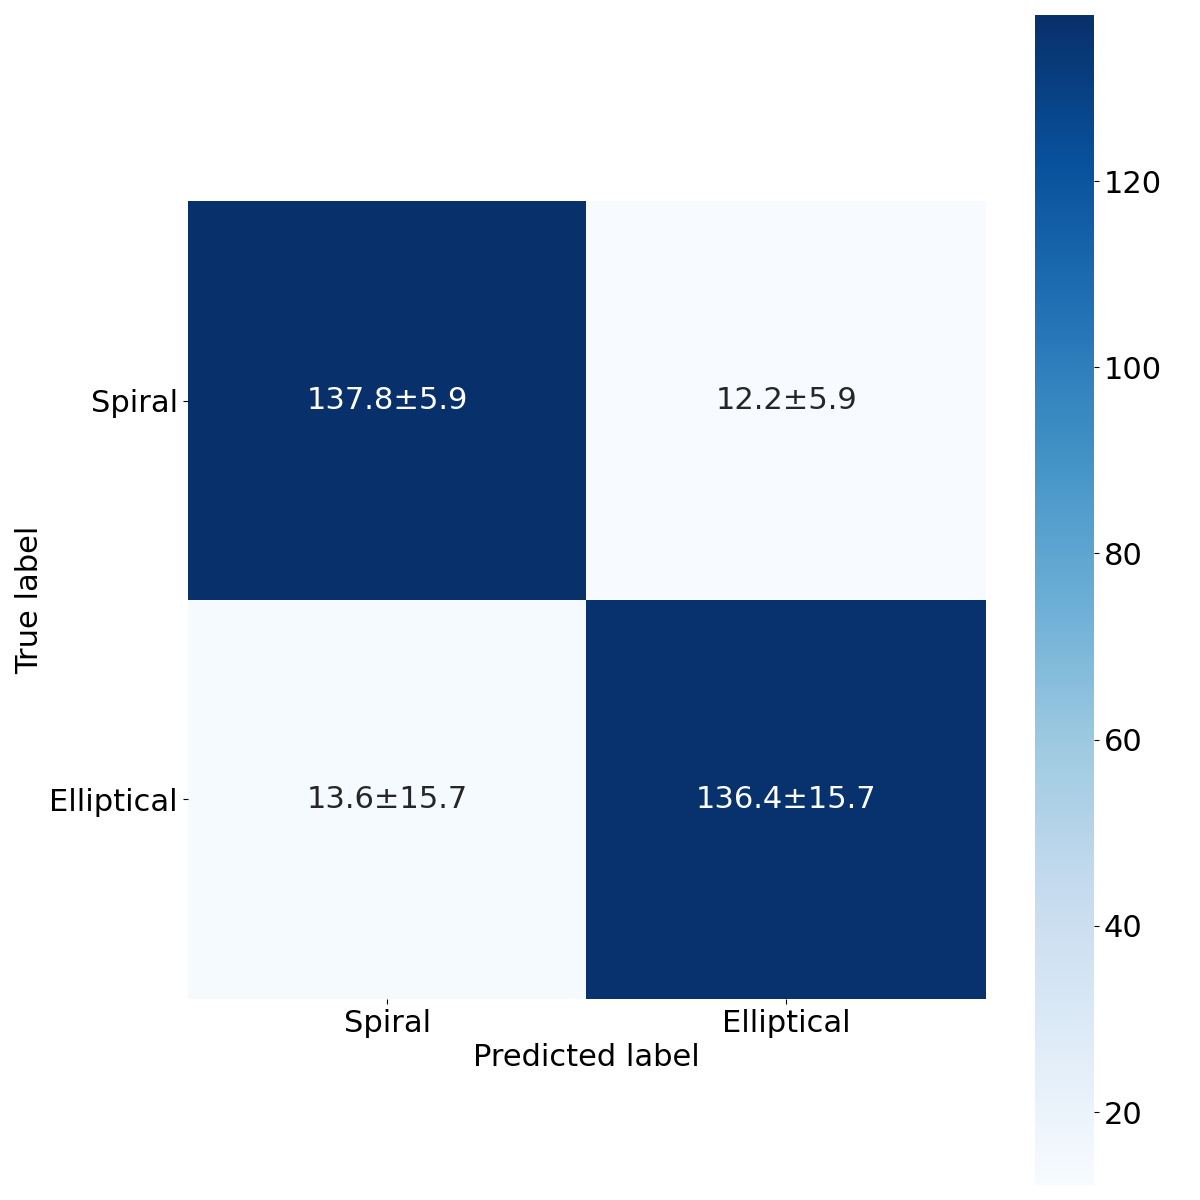
\includegraphics[keepaspectratio, width=7cm]{images/cm_mean_std_ex4-3.png}
    \caption{バランスドデータ : 混同行列\\(平均$\pm$標準偏差(1$\sigma$))}
		\label{fig:cm_ex4-3}
  \end{minipage}
\end{figure}

\subsubsection{結果}
\paragraph{モデル学習の進行}
図\ref{fig:losses_ex4-2-2}・図\ref{fig:accs_ex4-2-2}において,テストデータに対するスコアが100epoch付近までloss関数は降下,accuracyは上昇するものの,それ以降のepochではloss関数は上昇するがaccuracyは横ばいになっている.このことから,インバランスドデータで学習を行ったモデルは100epoch目以降学習データに対し過適合はしているものの,テストデータに対する汎化性能は失っていないことが読み取れる.

また図\ref{fig:losses_ex4-3}・図\ref{fig:accs_ex4-3}において,テストデータに対するスコアが75epoch付近までloss関数は降下,accuracyは上昇するものの,それ以降のepochではloss関数は上昇するがaccuracyは横ばいになっている.このことから,バランスドデータで学習を行ったモデルは75epoch目以降学習データに対し過適合はしているものの,テストデータに対する汎化性能は失っていないことが読み取れる.

\paragraph{テストデータに対するaccuracyの評価}
モデルの形態分類性能を評価するため,両モデル間にてテストデータに対する予測のaccuracyの比較を行う.性能評価においては,モデルが学習しきった際の分類性能を用いる.すなわち,accuracyを採るepoch数は,テストデータに対するaccuracyが最大となるepoch数とした.


インバランスドデータで学習を行ったモデル,およびバランスドデータで学習を行ったモデルにおける,テストデータへの予測精度(accuracy)を表\ref{tb:accs_4.3}に示す.両モデルにて,accuracyを採るepoch数を表内に示している.表\ref{tb:accs_4.3}において,1行目には今回の30回実行におけるaccuracyの平均値と標準偏差,2行目にはaccuracyの平均値と今回の30回実行から推定した標準誤差をそれぞれ2$\sigma$分記載した.

表\ref{tb:accs_4.3}より,テストデータに対する予測のaccuracyの標準誤差付き平均値においてインバランスデータで学習を行ったモデルとバランスドデータで学習を行ったモデルとの間に有意な差はなかった.

\paragraph{TSSの導出方法,および両分類モデルの分類性能評価}
データセット内の分類ラベルのインバランス性に左右されづらい評価指標であるTSSにて,再度両モデルの評価・性能比較を行う.

TSSを導出するため,先ほど求めた「モデルが学習しきった地点と思われる,テストデータに対するaccuracyが最大となるepoch数」まで,再度30回学習およびテストを両モデルにて行った.今回行ったこの再度30回学習およびテストをした結果は,後ほど混同行列の導出にも用いる.

インバランスドデータで学習を行ったモデル,およびバランスドデータで学習を行ったモデルにおける,テストデータへの予測精度(TSS)を表\ref{tb:TSS_4.3}に示す.1行目には今回の30回実行におけるTSSの平均値と標準偏差,2行目にはTSSの平均値と今回の30回実行から推定した標準誤差をそれぞれ2$\sigma$分記載した.表\ref{tb:TSS_4.3}より,\textbf{標準誤差付き平均値を見たとき,TSSが両モデルとも0.8付近と高いスコアを記録しており,また両モデルにおける有意差はなかった.このことから,両モデルとも渦巻銀河と楕円銀河をそれぞれ正しく分類する能力を持っており,またモデル学習において渦巻銀河・楕円銀河どちらの特徴もある程度正しく学習できていることが分かる.}

\paragraph{混同行列によるモデルの評価}
TSS導出に用いた「モデルが学習しきった地点と思われる,テストデータに対するaccuracyが最大となるepoch数まで,再度モデルの30回学習及びテスト」の結果を用い,両モデルの混同行列を導出した.導出された混同行列をそれぞれ図\ref{fig:cm_ex4-2-2},図\ref{fig:cm_ex4-3}に示す.図にはそれぞれ個数の平均値と標準偏差が1$\sigma$で示されている.

図\ref{fig:cm_ex4-2-2}より,インバランスドデータを用いて学習を行ったモデルにおいて陽性を渦巻銀河とした場合のtrue positive rateは0.948,楕円銀河とした場合は0.842であることが分かる.また図\ref{fig:cm_ex4-3}より,バランスドデータを用いて学習を行ったモデルにおいて陽性を渦巻銀河とした場合のtrue positive rateは0.919,楕円銀河とした場合は0.909であることが分かる.

\begin{table}[htbp]
  \centering
	\caption{インバランスドデータで学習を行ったモデル,およびバランスドデータで学習を行ったモデルのテストデータに対する予測のaccuracy}
  \begin{tabular}{|c|c|c|}
		\hline
    & mean$\pm$std (2$\sigma$) & mean$\pm$ste (2$\sigma$) \\ \hline
    インバランスドデータでのモデル & $0.931 \pm 0.034$(158th epoch) & $0.931 \pm 0.006$(158th epoch) \\ \hline
    バランスドデータでのモデル & $0.922 \pm 0.036$(123th epoch) & $0.922 \pm 0.007$(123th epoch) \\ \hline
  \end{tabular}
  \label{tb:accs_4.3}
\end{table}

\begin{table}[htbp]
  \centering
	\caption{インバランスドデータで学習を行ったモデル,およびバランスドデータで学習を行ったモデルのテストデータに対する予測のTSS}
  \begin{tabular}{|c|c|c|}
		\hline
    & mean$\pm$std (2$\sigma$) & mean$\pm$ste (2$\sigma$) \\ \hline
    インバランスドデータでのモデル & $0.791 \pm 0.250$ & $0.791 \pm 0.046$ \\ \hline
    バランスドデータでのモデル & $0.828 \pm 0.184$ & $0.828 \pm 0.033$ \\ \hline
  \end{tabular}
  \label{tb:TSS_4.3}
\end{table}

\section{4章全体の議論・結論}
4.2節の実験にて,不確かな天体を入れた3値分類問題とした方がテストデータに対する予測精度が落ちてしまう現象が確認された.この現象の理由としては,不確かな天体がGZにて形態ラベル付けを行った人間にとっては分類できず,深層学習分類モデルにとっては分類できるほどの特徴を有していることが推測される.分類モデルには渦巻銀河・楕円銀河のどちらかに分類できる天体に「不確かな天体」というラベル付けがされているため,モデルが渦巻銀河・楕円銀河・不確かな天体を3つに分類できるような学習がされないのではないかと考えられる.もし不確かな天体と分類されている天体に正確なラベル付けが行われれば,深層学習分類モデルの分類精度は向上するものと思われる.


4.3節の実験にて,学習・テストに用いるデータ内のインバランス改善を行っても精度が改善しなかった理由について,これはインバランスドデータ内にてよりデータ数の少ない楕円銀河においても,テストデータ内の楕円銀河を分類する能力獲得に十分なデータ数および特徴の多様性が存在していたことが考えられる.もし学習データ内にて桁数が異なるほどの強いデータインバランスが起きていた場合,データインバランス改善を行えば分類精度が改善される可能性がある.

4章の目標は「学習データとテストデータの解像度が等しい」という条件にて,高精度分類が行えるモデルを学習させることであった.この目標を達成するため,2つの実験を行った.GZにて不確かと分類されている天体を除外し,渦巻銀河・楕円銀河の2値分類問題とすることで,分類モデルの分類精度は大きく向上した.また,学習・テストに用いるデータ内のデータインバランスを改善しても分類精度に有意差が認められるほどの向上は見受けられなかった.当論文における今後の実験では,渦巻銀河を見分けることに特化したモデルでなく,渦巻銀河・楕円銀河の両者を分類することを優先するため,渦巻銀河・楕円銀河の両者の真陽性率向上が見込めるバランスドデータにてモデル学習を行っていく.



\newpage
\chapter{空間解像度差のあるデータセットを用いた分類モデル学習}
当論文の将来展望は,高空間分解能観測装置データを用いてモデル学習を行うことで,既存の低空間分解能データセットに対し更なる高精度形態分類を提供するというものである.この将来展望の前提条件である,学習データとテストデータとの間の解像度が揃っているデータセットにて高精度の銀河形態分類モデルを学習させることを,第4章にて達成することができた.

そこで,この章では将来展望で行われる予定の「異なる観測装置データの組み合わせ」を念頭に置き,学習データとテストデータとの間に解像度差があるデータセットにて形態分類モデルの学習が行えるかを検証する.

具体的には,以下の事項を検証するため,2つの実験を行った.

\begin{quote}
 \begin{itemize}
  \item 学習データとテストデータとの間に解像度差があるデータセットにて形態分類モデルを学習し,
  \begin{quote}
   \begin{itemize}
    \item テストデータへの予測が成立するか
    \item 予測が成立する場合,解像度差がいくつまでならば使用可能か
   \end{itemize}
  \end{quote}
 \end{itemize}
\end{quote}

\section{実験概要}
第5章ではSDSSから取得した銀河切り出し画像とGZから取得した分類フラグを学習データとしてモデルを学習させ,銀河切り出し画像を縮小した低解像度データセットに対し予測を行う.なお,学習・テストに用いる天体データの銀河種は渦巻銀河・楕円銀河の2つとする.
\subsubsection{学習データ}
学習に用いる画像データは,SDSSから取得した64ピクセル四辺の銀河切り出し画像を使用し,正解ラベルはGZから取得した分類フラグを用いる.実験には15,000天体を用いた.15,000天体の赤方偏移別の個数を示したグラフを図\ref{fig:z_15000_2}に示す.一般的に赤方偏移の値が小さいほど,地球から近い天体といえる.15,000天体のうち,GZの分類フラグにて渦巻銀河と分類されている天体は4,058天体,楕円銀河は1,561天体であった.

モデルの学習および評価の際,モデルの学習データとテストデータの比率は7:3とした.

\begin{figure}[h]
 \centering
 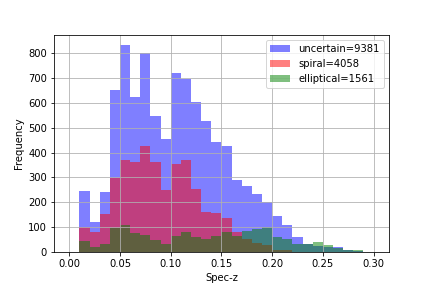
\includegraphics[width=14cm]{images/z_15000_4.png}
 \caption{実験に用いる15,000天体の赤方偏移別の個数グラフ}
 \label{fig:z_15000_2}
\end{figure}

\subsubsection{縮小画像データセット(テストデータ)の作成方法}
この章ではテストデータとして,SDSSから取得した銀河切り出し画像を縮小したデータセットを使用する.SDSSから取得した15,000天体(図\ref{fig:z_15000_2}参照)を平均画素法により縮小処理を施した.画像の縮小にはOpenCV\ref{}に実装されているresize関数の''INTER\_AREA''メソッドを使用した.銀河切り出し画像を1/2倍から1/8倍に縮小し,計7つの縮小画像データセットを作成した.縮小画像の例として,1/4倍に縮小した画像群を図\ref{fig:shrink_1_4}に示す.

\begin{figure}
 \centering
 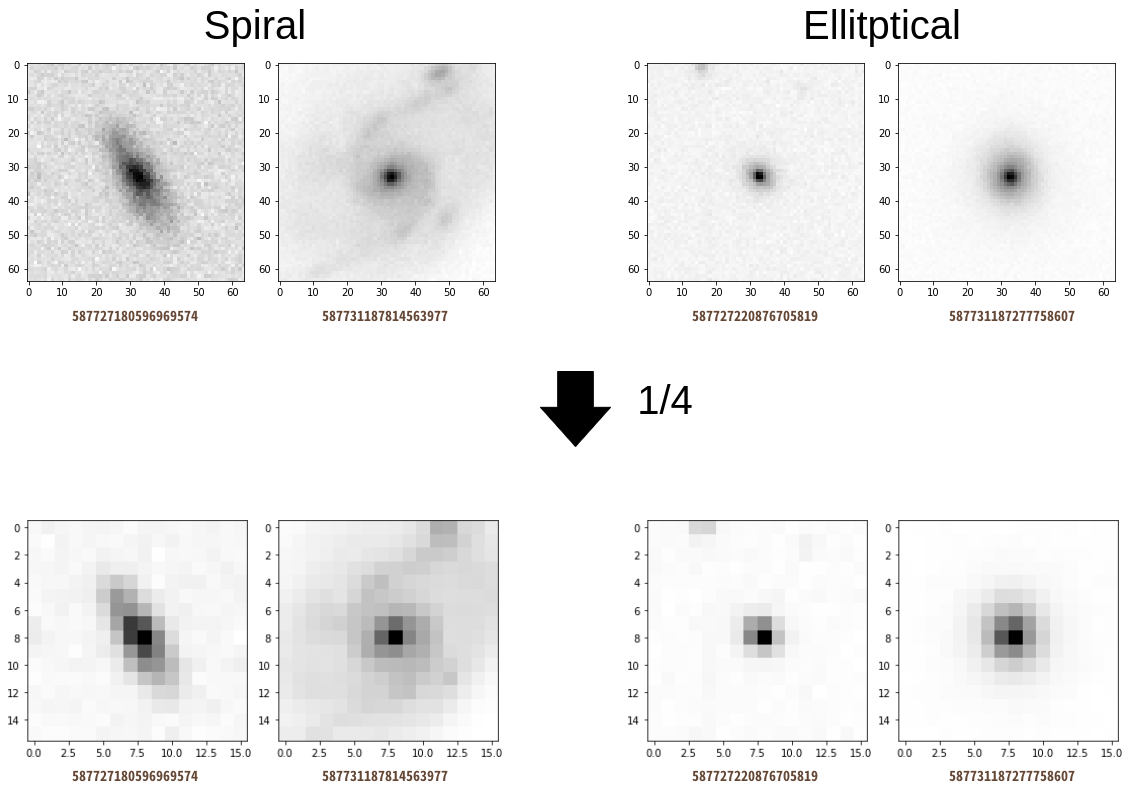
\includegraphics[width=13cm]{images/5syou/syuron_5syou_kakudai/ver1/5syou_shrink_ver1.png}
 \caption{銀河切り出し画像の縮小例(1/4倍)}
 \label{fig:shrink_1_4}
\end{figure}

\subsubsection{縮小画像データセットの内挿方法}
モデルに画像データを入力する際,用いる画像サイズは揃えて入力する必要がある.第5章では学習データとテストデータとの間で画像サイズが異なる.そのため,今回の実験ではテストデータである縮小画像データセットを拡大して
モデルに入力する.

縮小画像の拡大には,OpenCVのresize関数を用いた.この章での実験において,画像拡大の際の補間方法として最近傍補間,バイリニア補間,バイキュービック補間を使用した.画像拡大の例として,1/4倍に縮小された銀河切り出し画像の,各補間方法による画像拡大の例を図\ref{fig:kakudai_1_4}に示す.なお図\ref{fig:kakudai_1_4}にて用いられている縮小画像は,図\ref{fig:shrink_1_4}のものと同様である.

\begin{figure}
 \centering
 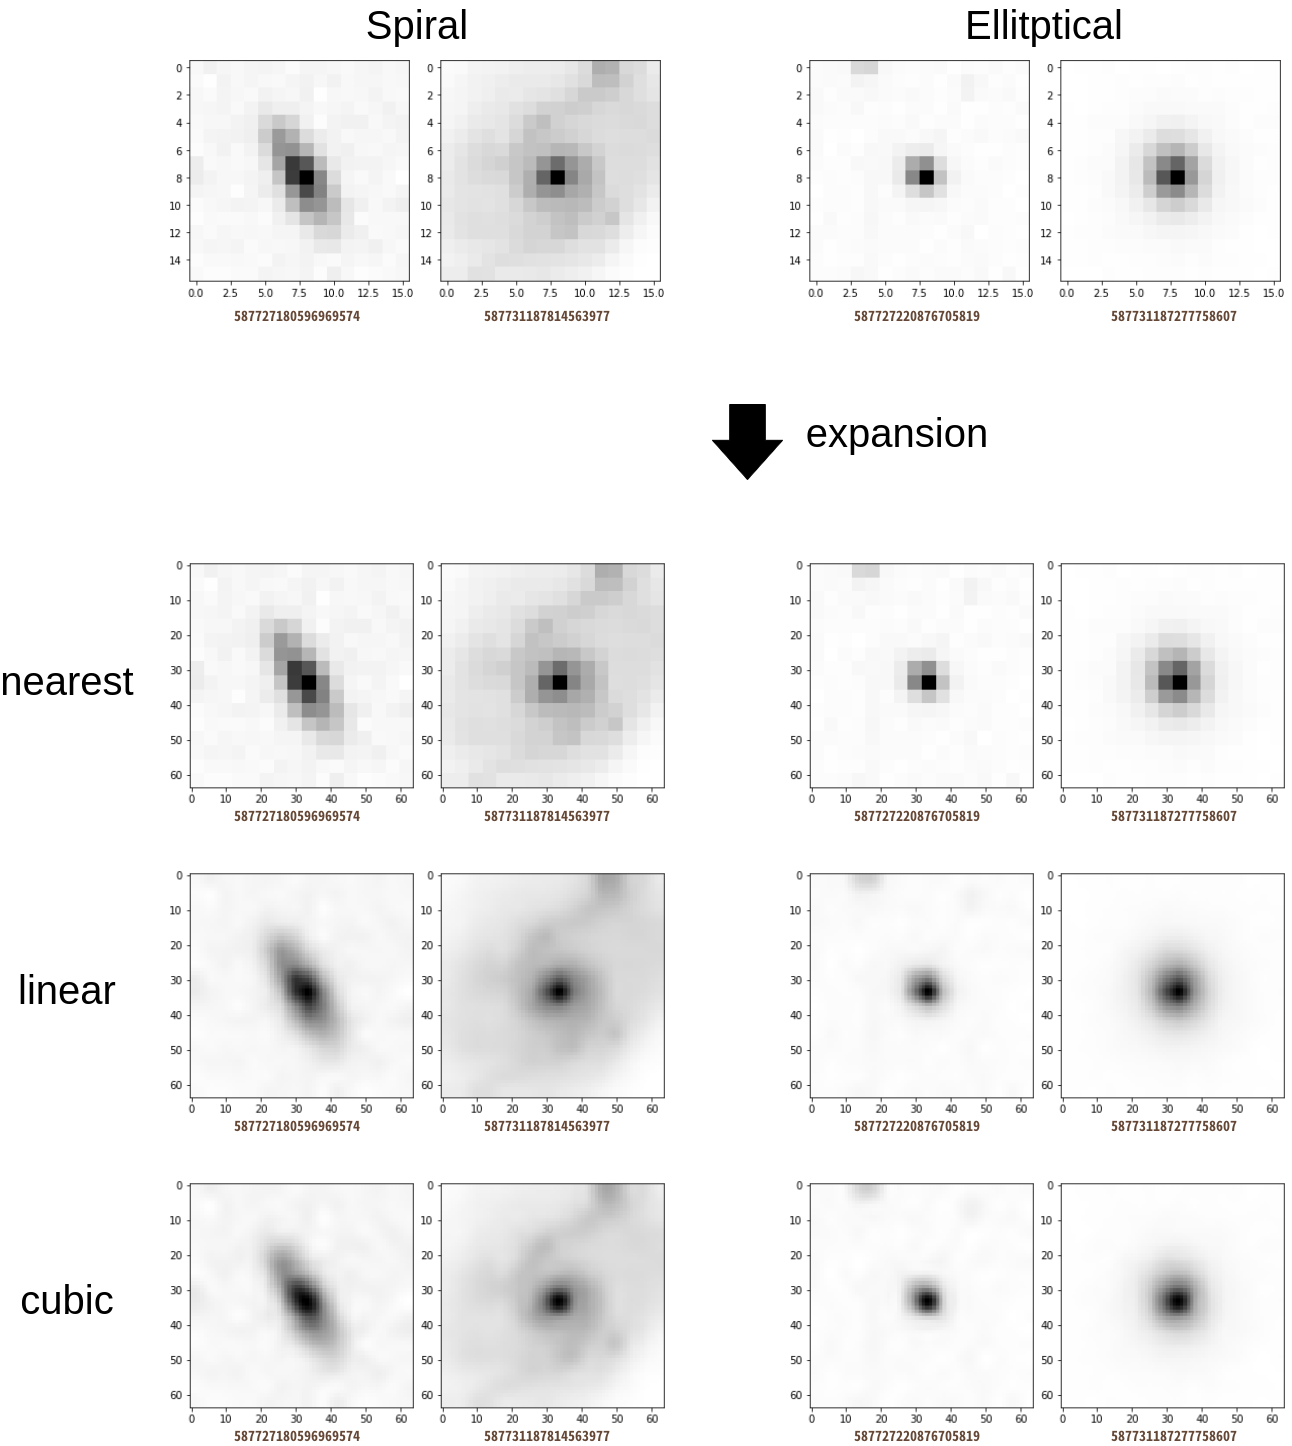
\includegraphics[width=13cm]{images/5syou/syuron_5syou_kakudai/ver1/5syou_kakudai_ver1.png}
 \caption{1/4倍縮小画像の画像拡大例//(最近傍補間・バイリニア補間・バイキュービック補間)}
 \label{fig:kakudai_1_4}
\end{figure}

\subsubsection{モデル構造}
今回用いた深層学習モデルは,cheng et al.(2019)\ref{Cheng2019}にて用いられていた銀河形態分類モデルを参考にした.今回用いたモデルの構造を図\ref{fig:model_shape_2}に示す.このモデルは畳み込み層を合計3つ有しており,それぞれのカーネルサイズは3x3, 3x3, 2x2である.それぞれの畳み込み層の後には,2x2のmax-pooling層が存在する.全畳み込み層の後に全結合層が2層配置されており,それぞれ1024個のノードを有している.

\begin{figure}[h]
	\centering
	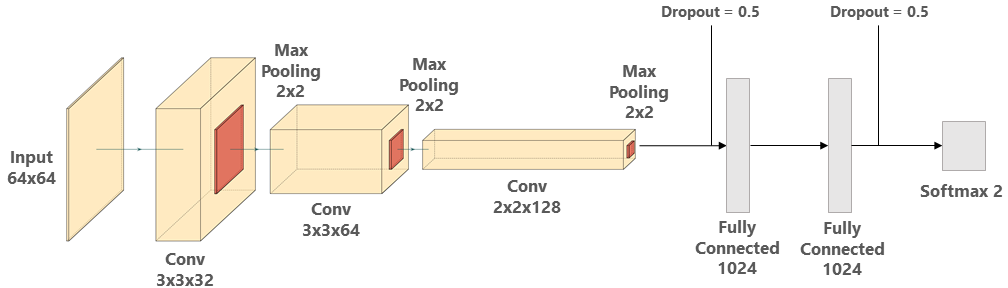
\includegraphics[width=14cm]{images/model_shape.png}
	\caption{用いた分類モデルの構造図}
	\label{fig:model_shape_2}
\end{figure}
 
\subsubsection{モデルの評価方法}
分類モデルの評価指標として,accuracy (正解率)を用いた.accuracyは全テストデータの中で正しく分類できたデータがどれだけあるかというものであり,モデルの正確性を表す指標である.

また,深層学習モデルには実行毎に学習のブレが存在するため,モデルの評価の際には学習・テストを30回実行し,評価指標の平均値,標準偏差および標準誤差を導出する.

\section{分類精度のデータセット内解像度差依存性}
この節では,学習データとテストデータとの間に解像度差がある状況において,
\begin{inparaenum}[(1)]
  \item テストデータへの予測が成立するか
  \item 予測が成立する場合,解像度差がいくつまでならば使用可能か
\end{inparaenum}
の検証を行う.このうち(2)において「使用可能」の定義として,学習データとテストデータの解像度が揃っている状況での予測結果である''Original''と同程度の高精度な分類,すなわちaccuracyが0.9付近を記録する結果であることとする.

\subsection{実験条件}
使用する天体は,GZによる形態分類が行われた15,000天体(図\ref{fig:z_15000}参照)を母集団とした.銀河種類ごとのデータインバランスが起こらないようにするため,その母集団の中から渦巻銀河と楕円銀河をそれぞれ300天体選定した.選定を行う際,赤方偏移$z$について,$0 < z < 0.2$という条件を設定し,あてはまらない天体は除外を行う.これは,地球との距離が遠すぎる天体については上手く特徴抽出が行えず学習の妨げになる可能性があるからである.

使用天体を渦巻銀河300天体,楕円銀河300天体の合計600天体を選定したあと,学習データとテストデータの比率が7:3となるように天体群を分けた.このうち,学習データにはSDSSの切り出し画像,テストデータにはSDSSの切り出し画像を縮小した画像をそれぞれ用いた.また,学習データとテストデータ内において,銀河種のデータインバランスが起こらないようにするため,渦巻銀河と楕円銀河の比率が等しくなるようにした.

モデルの評価を行う際,モデルの学習およびテストを30回行い,accuracyの平均値,標準偏差および標準誤差を導出した.
なお,30回の学習およびテストの際,学習実行毎に使用される天体は毎回シャッフルされる.

モデルの学習期間は900epochとした.これは,すべての縮小データの縮小倍率にて,モデルが学習しきる期間,すなわちテストデータに対するaccuracyが上がりきるepoch数が900epochであったからである.

\subsection{実験結果}
\subsubsection{縮小データに対する予測結果}
銀河切り出し画像を1/2倍から1/8倍に縮小した縮小データに対する,形態分類モデルの予測結果の図を図\ref{fig:nearest_300_1std}から図\ref{fig:inter_comparison_300_1std}に示す.

\begin{quote}
 \begin{itemize}
  \item 横軸が,テストデータである縮小データの縮小倍率であり,縦軸がテストデータに対する予測のaccuracyとなっている.
  \begin{quote}
   \begin{itemize}
    \item テストデータに対する予測のaccuracyについて,30回実行における平均値と標準偏差(2std)をエラーバー形式で示している.
    \item なお,一番左に位置しているOriginalとなっている箇所は,テストデータに縮小データでなく,学習データと同じ大きさの銀河切り出し画像を使用してテストを行った結果である.すなわち,Originalが学習データとテストデータの解像度が揃っている状況での予測結果に対し,1/2から1/8が学習データとテストデータとの間に解像度差がある状況での予測結果を示している.
   \end{itemize}
  \end{quote}
  \item accuracyを採るepoch数は,モデルが十分に学習しきるepoch数とした.すなわち,テストデータに対するaccuracyが最大値となるepoch数とした.
  \item 図\ref{fig:inter_comparison_300_1std}には,内挿方法間でのaccuracyの比較を図に示した.
 \end{itemize}
\end{quote}

\begin{figure}[H]
 \centering
 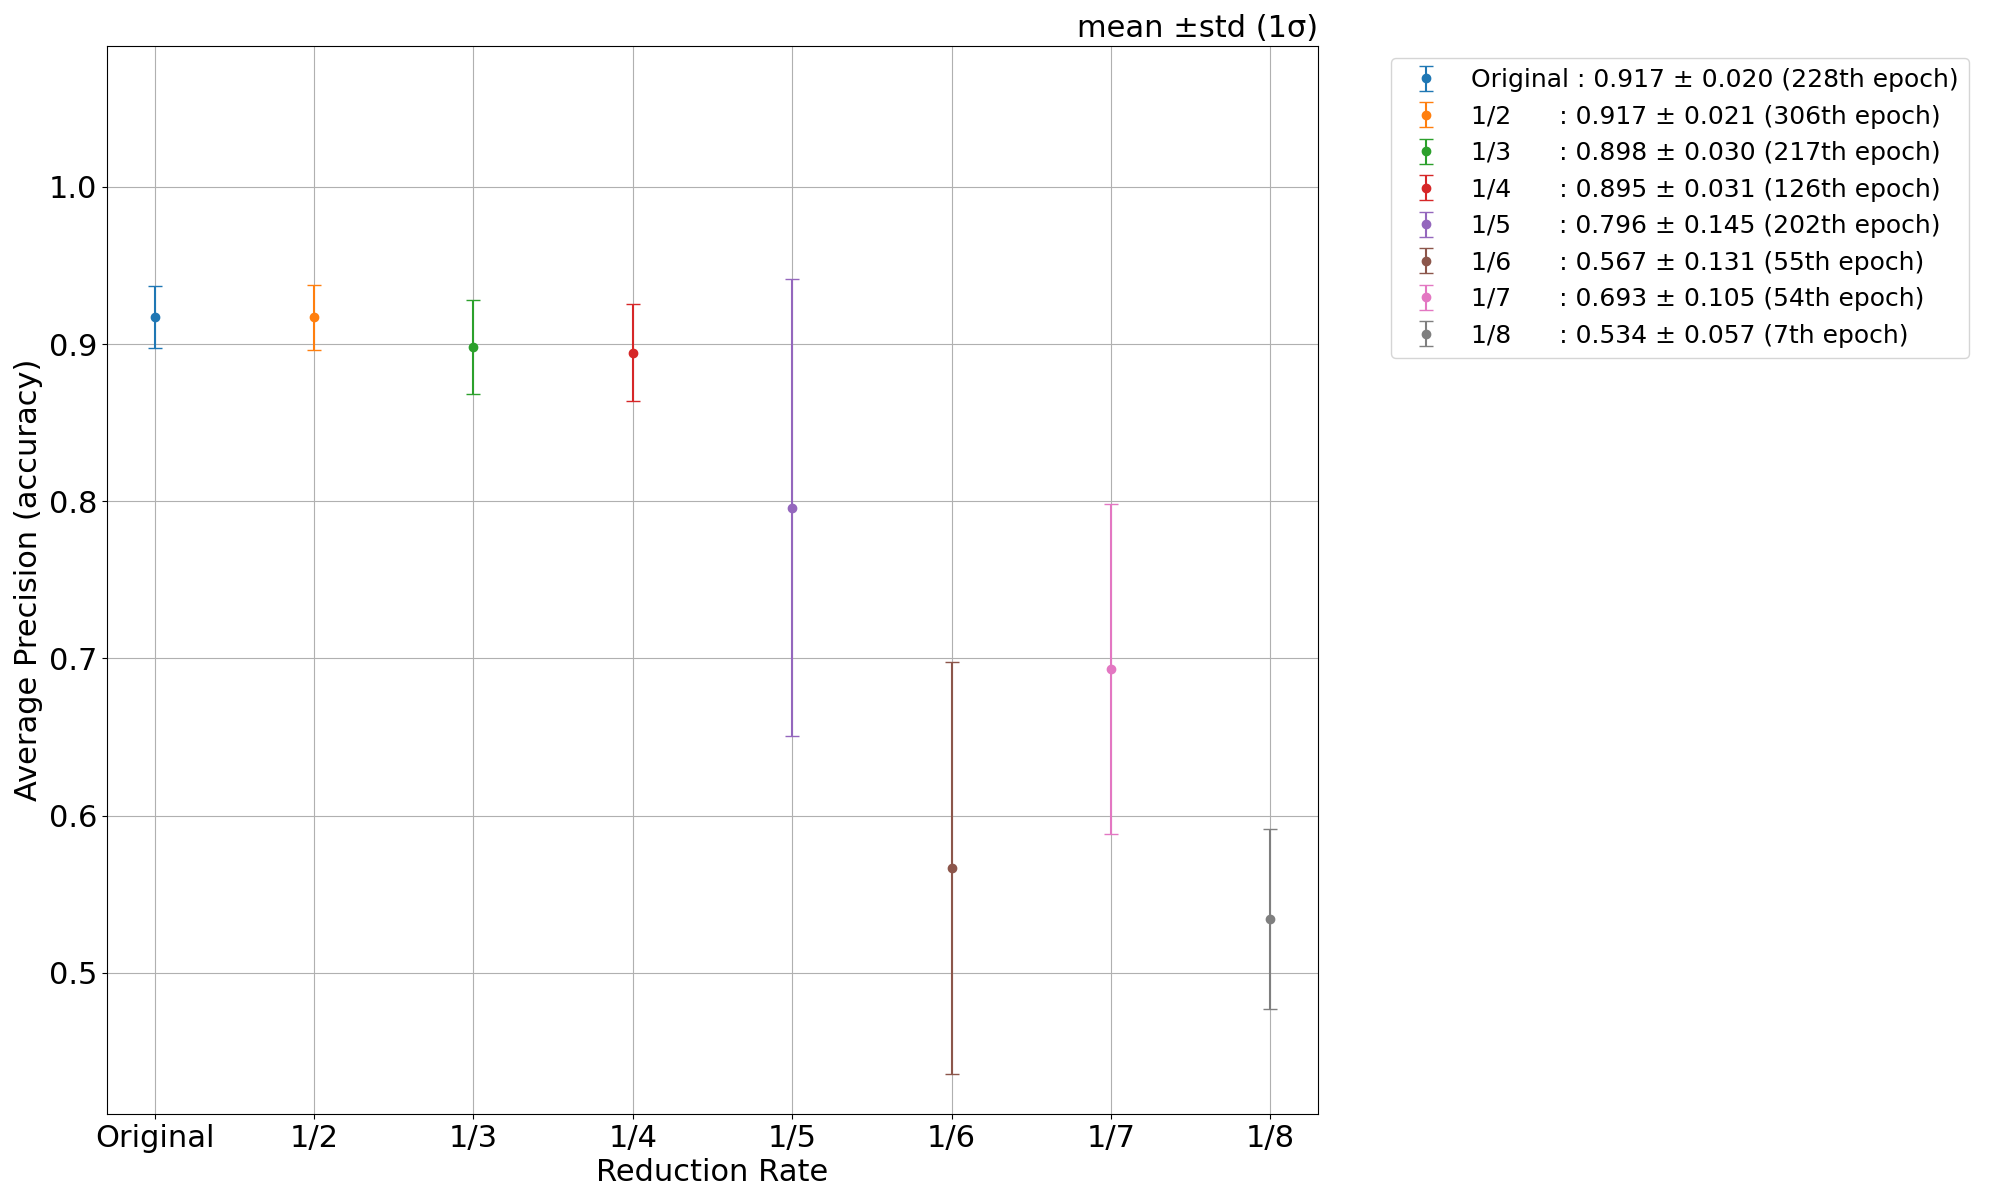
\includegraphics[width=16cm]{images/5syou/print_errorbar/nearest/acc_with_errorbar_syuron5_nearest_900epoch_30run_300_acc_max_std1sigma.png}
 \caption{最近傍補間によって内挿された,縮小データに対するモデルの予測結果(1std)}
 \label{fig:nearest_300_1std}
\end{figure}

\begin{figure}[H]
  \centering
  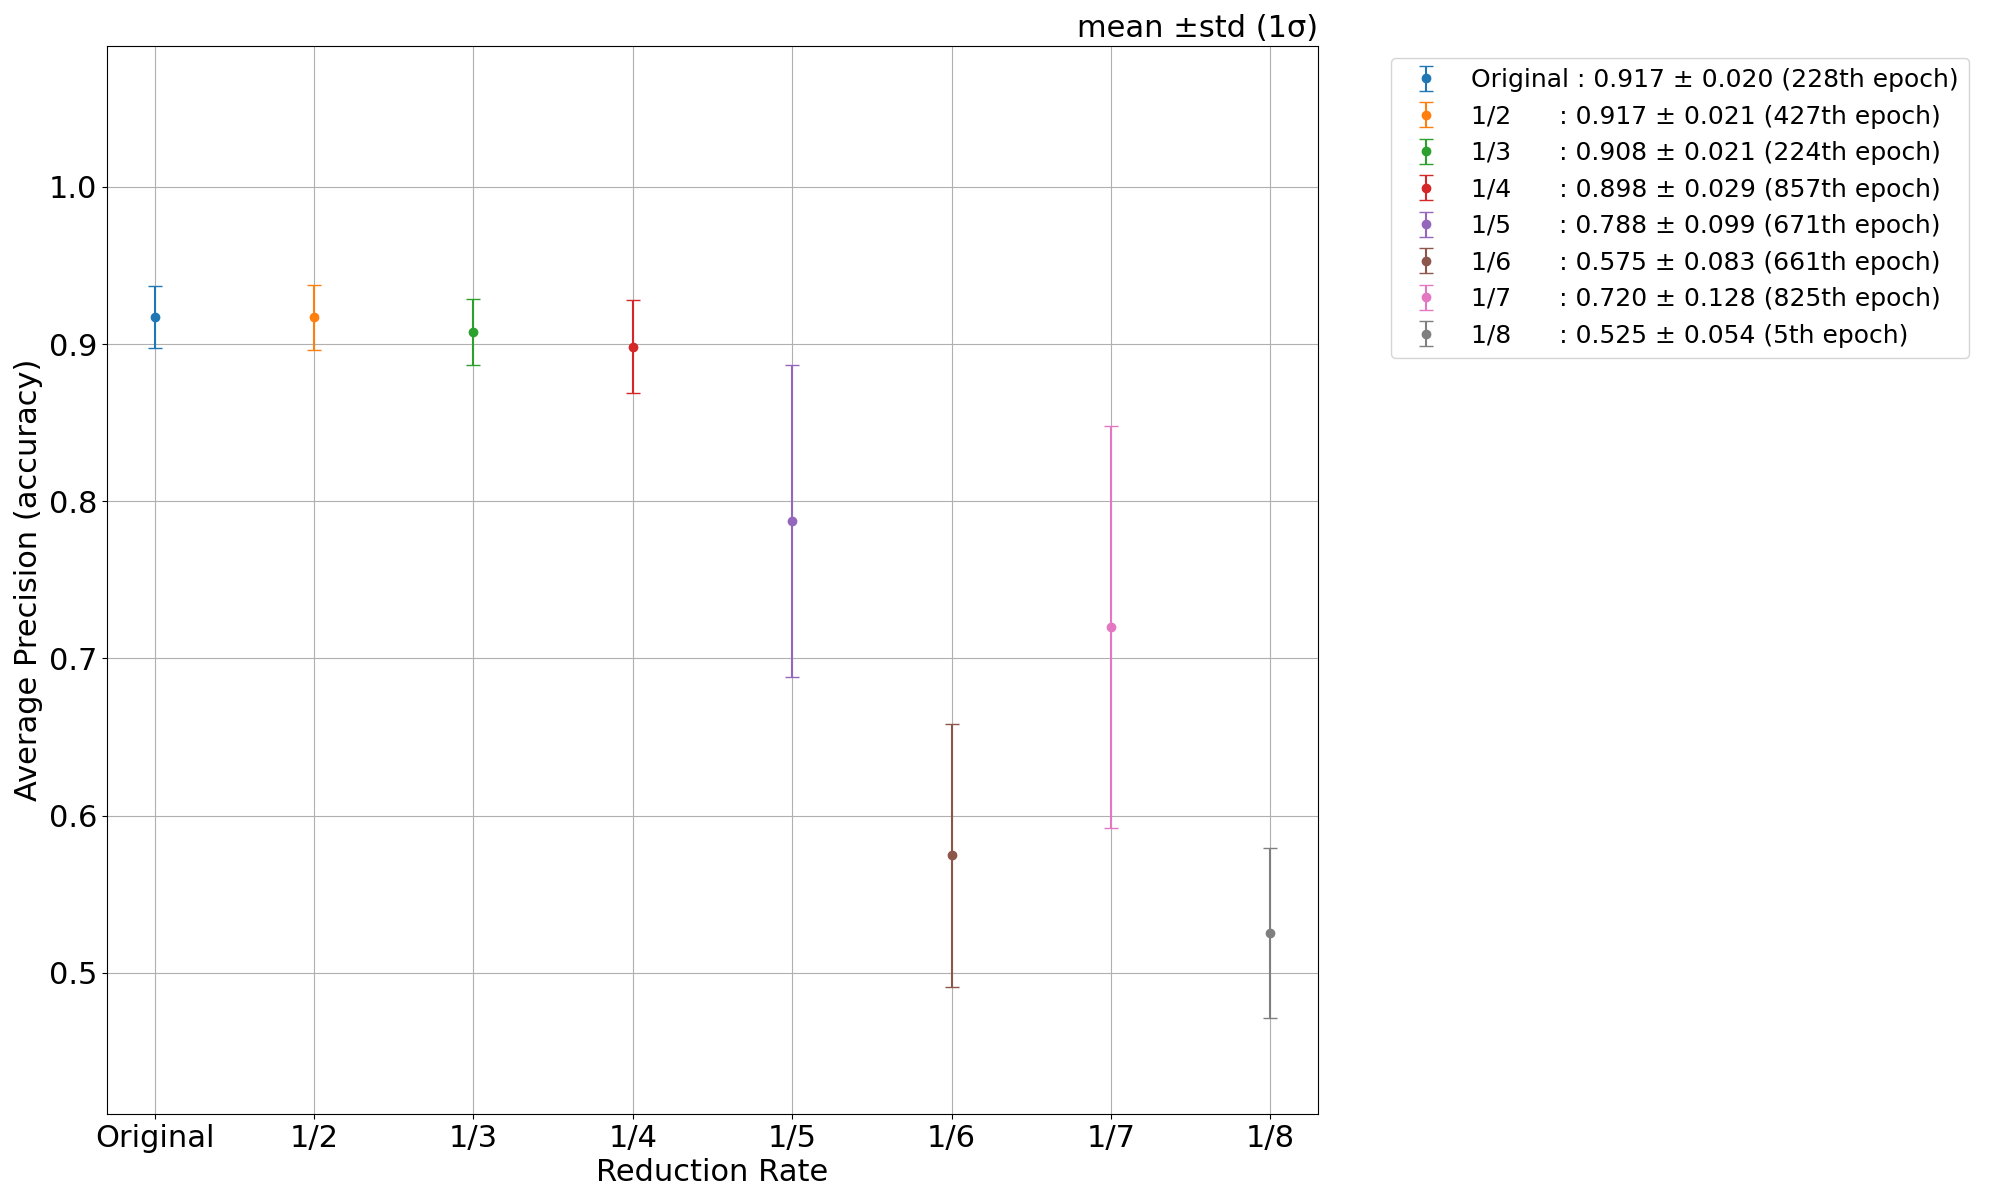
\includegraphics[width=16cm]{images/5syou/print_errorbar/linear/acc_with_errorbar_syuron5_linear_900epoch_30run_300_acc_max_std1sigma.png}
  \caption{バイリニア補間によって内挿された,縮小データに対するモデルの予測結果(1std)}
  \label{fig:linear_300_1std}
\end{figure}

\begin{figure}[H]
  \centering
  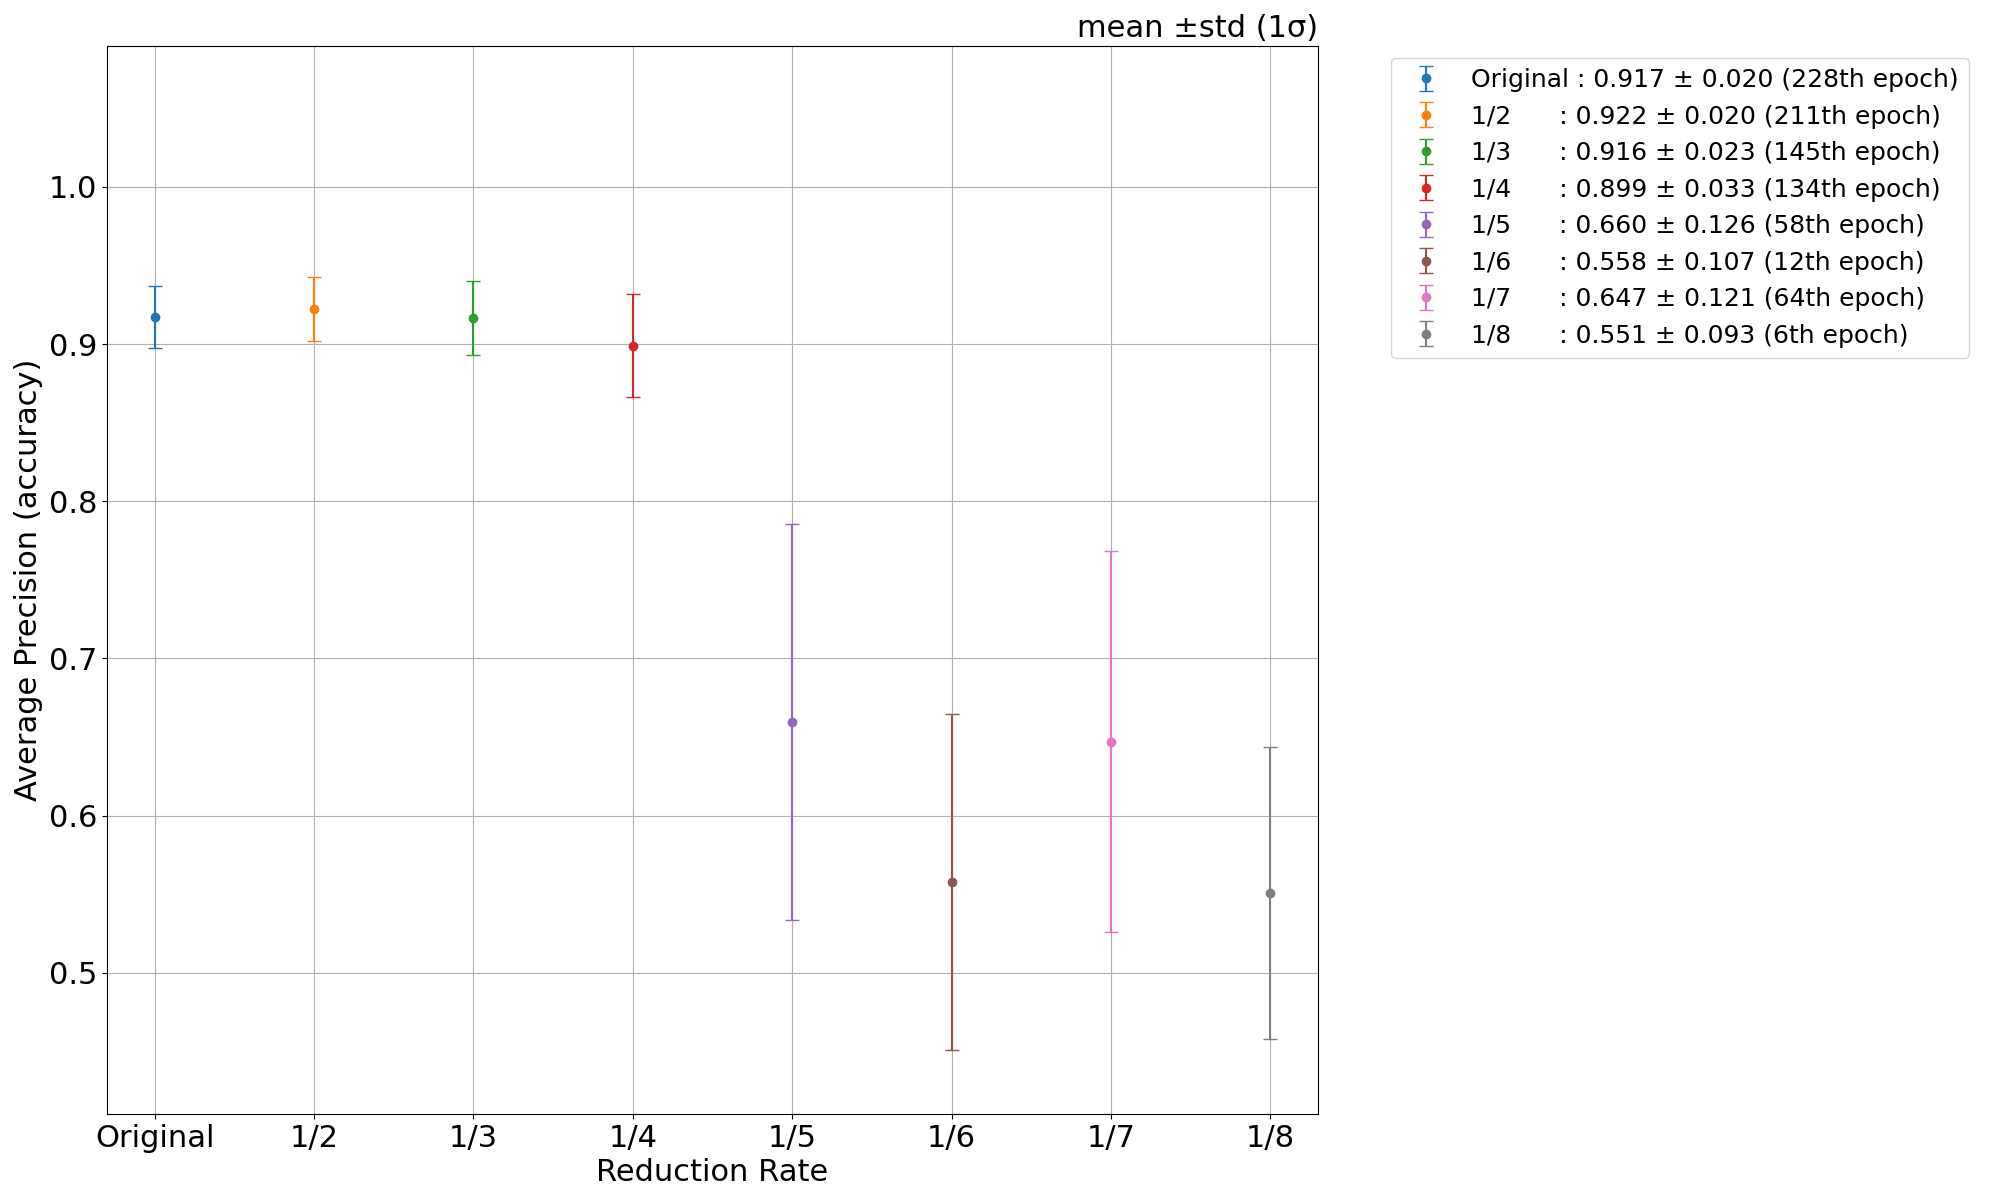
\includegraphics[width=16cm]{images/5syou/print_errorbar/cubic/acc_with_errorbar_syuron5_cubic_900epoch_30run_300_acc_max_std1sigma.png}
  \caption{バイキュービック補間によって内挿された,縮小データに対するモデルの予測結果(1std)}
  \label{fig:cubic_300_1std}
\end{figure}

\begin{figure}[H]
  \centering
  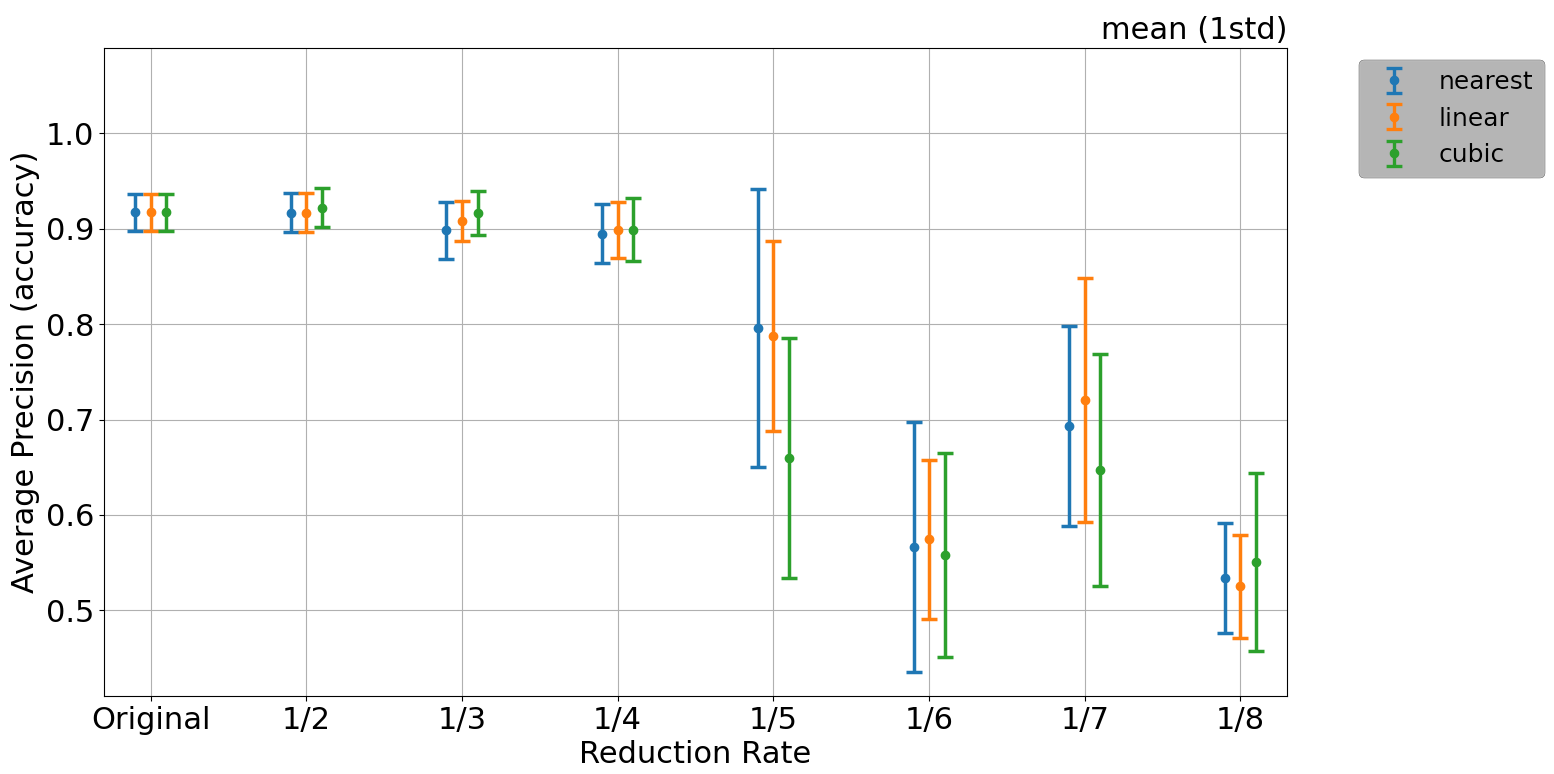
\includegraphics[width=16cm]{images/5syou/print_errorbar/print_errorbar_inter_comparison/acc_with_errorbar_syuron5_inter_comparison_900epoch_30run_300_acc_max_std1sigma.png}
  \caption{内挿方法間での比較(1std)}
  \label{fig:inter_comparison_300_1std}
\end{figure}


\subsubsection{結果}
\paragraph{縮小データの縮小倍率における結果}
図\ref{fig:nearest_300_1std},図\ref{fig:linear_300_1std},図\ref{fig:cubic_300_1std}より,Originalの結果(学習データとテストデータの解像度が揃っている状況での予測結果)と同程度かつaccuracyが0.9付近を記録しているテストデータの縮小倍率が存在することが分かる.

図\ref{fig:nearest_300_1std}より,最近傍補間によって拡大したテストデータに対する予測は,縮小倍率が1/2から1/4倍の縮小データに対しては使用可能であることが分かる.なお,縮小倍率が1/5倍の縮小データに対する予測においては,accuracyが0.9を記録するモデルは1標準偏差区間において上位約17\%程しかなく,モデルの学習にかなりの上振れが起こらないと達成できないスコアであることから,使用可能ではないとの判断を行った.

同様に,図\ref{fig:linear_300_1std}よりバイリニア補間によって拡大したテストデータに対する予測は,縮小倍率が1/2から1/4倍の縮小データに対しては使用可能であり,また図\ref{fig:cubic_300_1std}よりバイキュービック補間によって拡大したテストデータに対する予測は,縮小倍率が1/2から1/4倍の縮小データに対しては使用可能であることが分かる.\\このことから,内挿方法によらず,学習データとテストデータの解像度差が1/4倍までであったら,テストデータとして使用可能であることが分かった.

\paragraph{内挿方法間での比較}
内挿方法の間で,テストデータに対するaccuracyの細かい挙動を比較する.図\ref{fig:inter_comparison_300_1std}より,1/2から1/4倍,および1/6から1/8倍の縮小データにおいては,1標準偏差の誤差区間において内挿方法による有意差は見受けられない.また,1/5倍の縮小倍率においてはバイキュービック補間によって内挿したテストデータに対する予測のaccuracyが他2手法より劣って見えるが,1標準偏差の誤差区間においては他2手法との有意差は見られない.このことから,テストデータへの予測のaccuracyにおいて,テストデータの内挿方法における有意差はないことが分かった.

\paragraph{標準誤差(1std)における予測結果}
図\ref{fig:nearest_300_1std}から図\ref{fig:cubic_300_1std}では,標準偏差(1std)を示した.ここで,標準誤差(1ste)の結果を図\ref{fig:nearest_300_1ste}から図\ref{fig:cubic_300_1ste}に示す.

1標準偏差(図\ref{fig:nearest_300_1std}から図\ref{fig:cubic_300_1std})と比べると,1標準誤差の誤差区間では各縮小倍率間で有意差が生じる.例として,図\ref{fig:nearest_300_1ste}を見ると,1標準偏差の誤差区間では有意差がなかった1/2倍と1/3倍の縮小データに対するaccuracyに,有意差が生じていることが読み取れる.このことから,深層学習において1つ1つのモデル学習にかなりのブレがあることがわかる.



\begin{figure}[H]
  \centering
  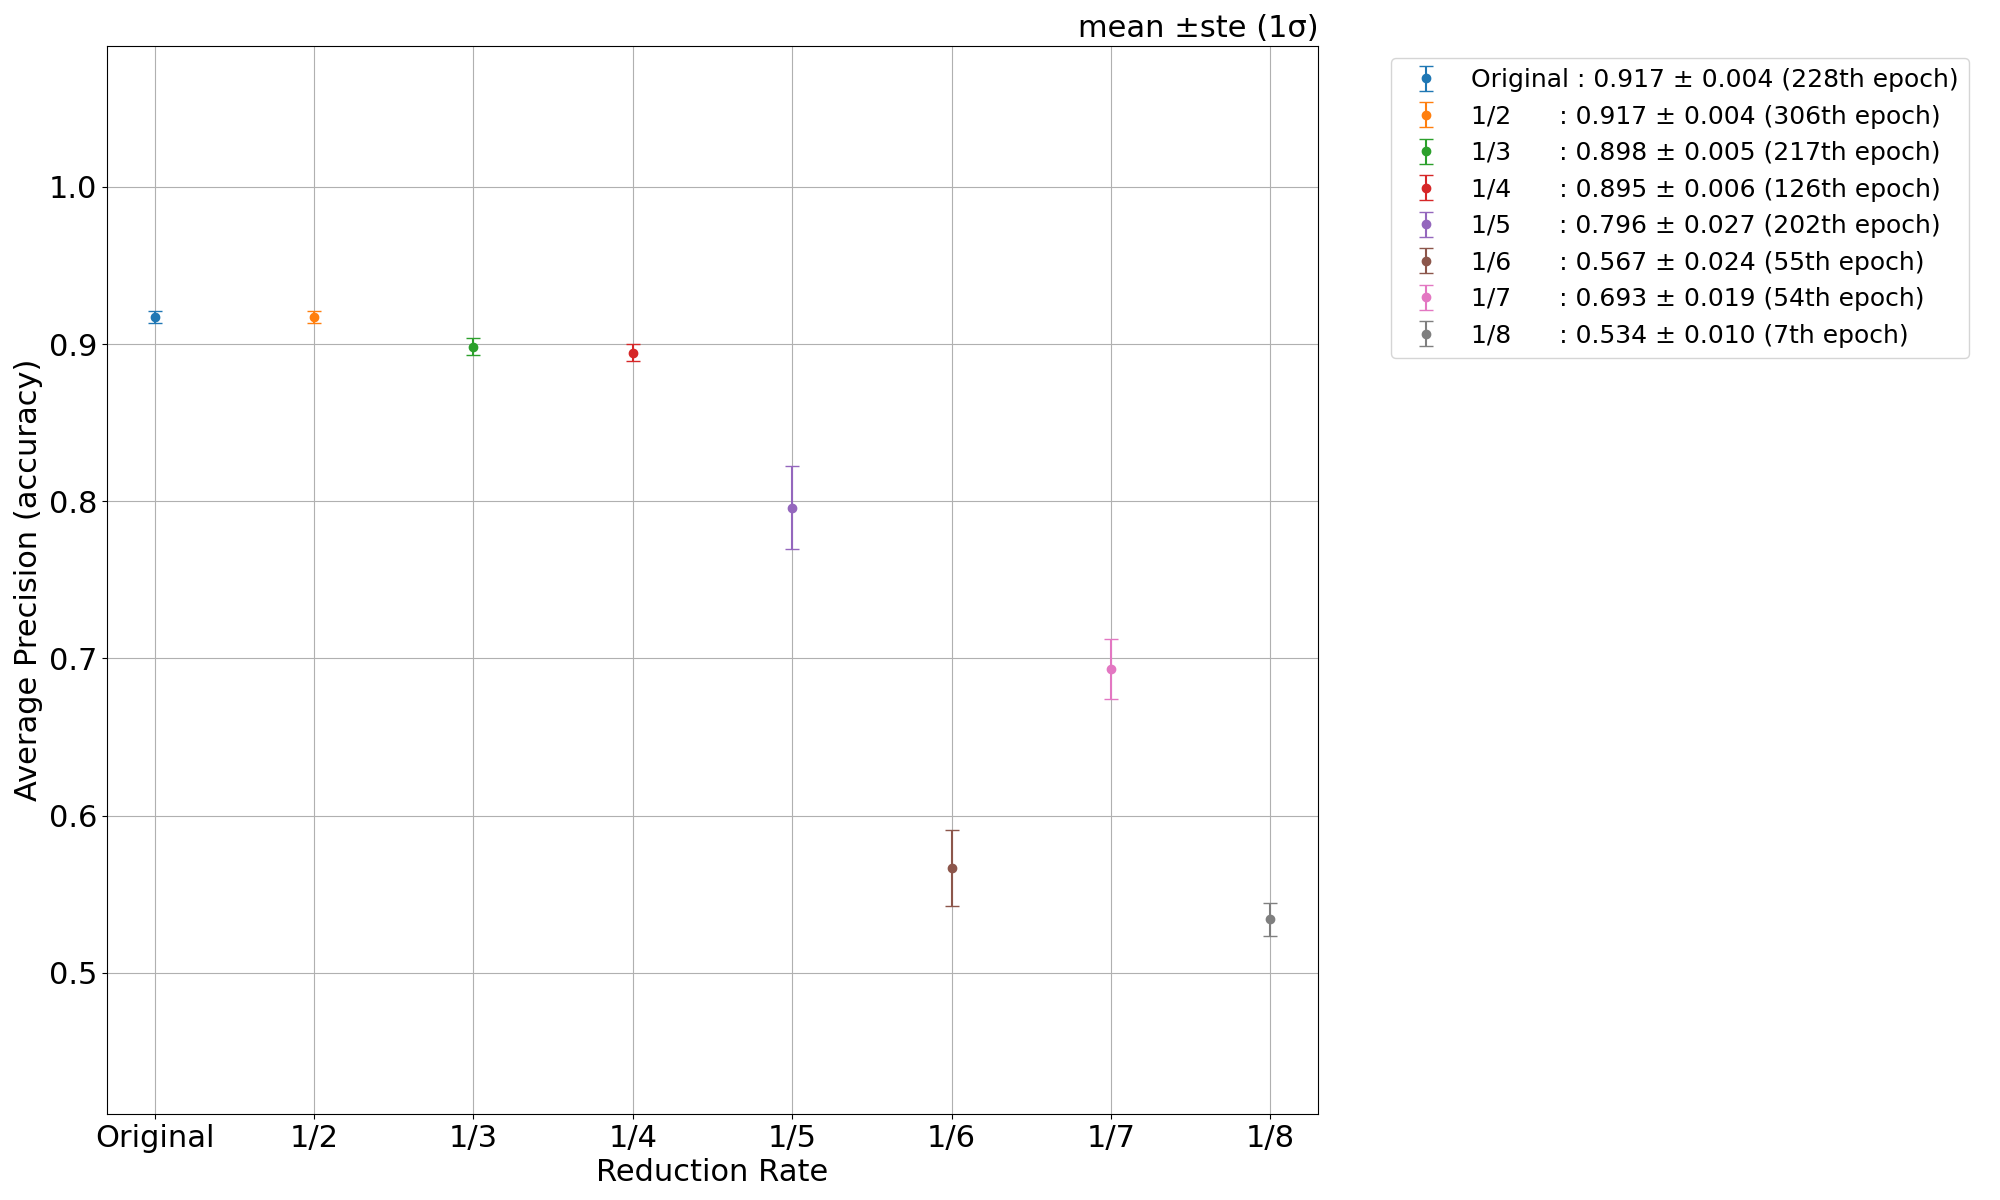
\includegraphics[width=16cm]{images/5syou/print_errorbar/nearest/acc_with_errorbar_syuron5_nearest_900epoch_30run_300_acc_max_ste1sigma.png}
  \caption{最近傍補間によって内挿された,縮小データに対するモデルの予測結果(1ste)}
  \label{fig:nearest_300_1ste}
\end{figure}

\begin{figure}[H]
  \centering
  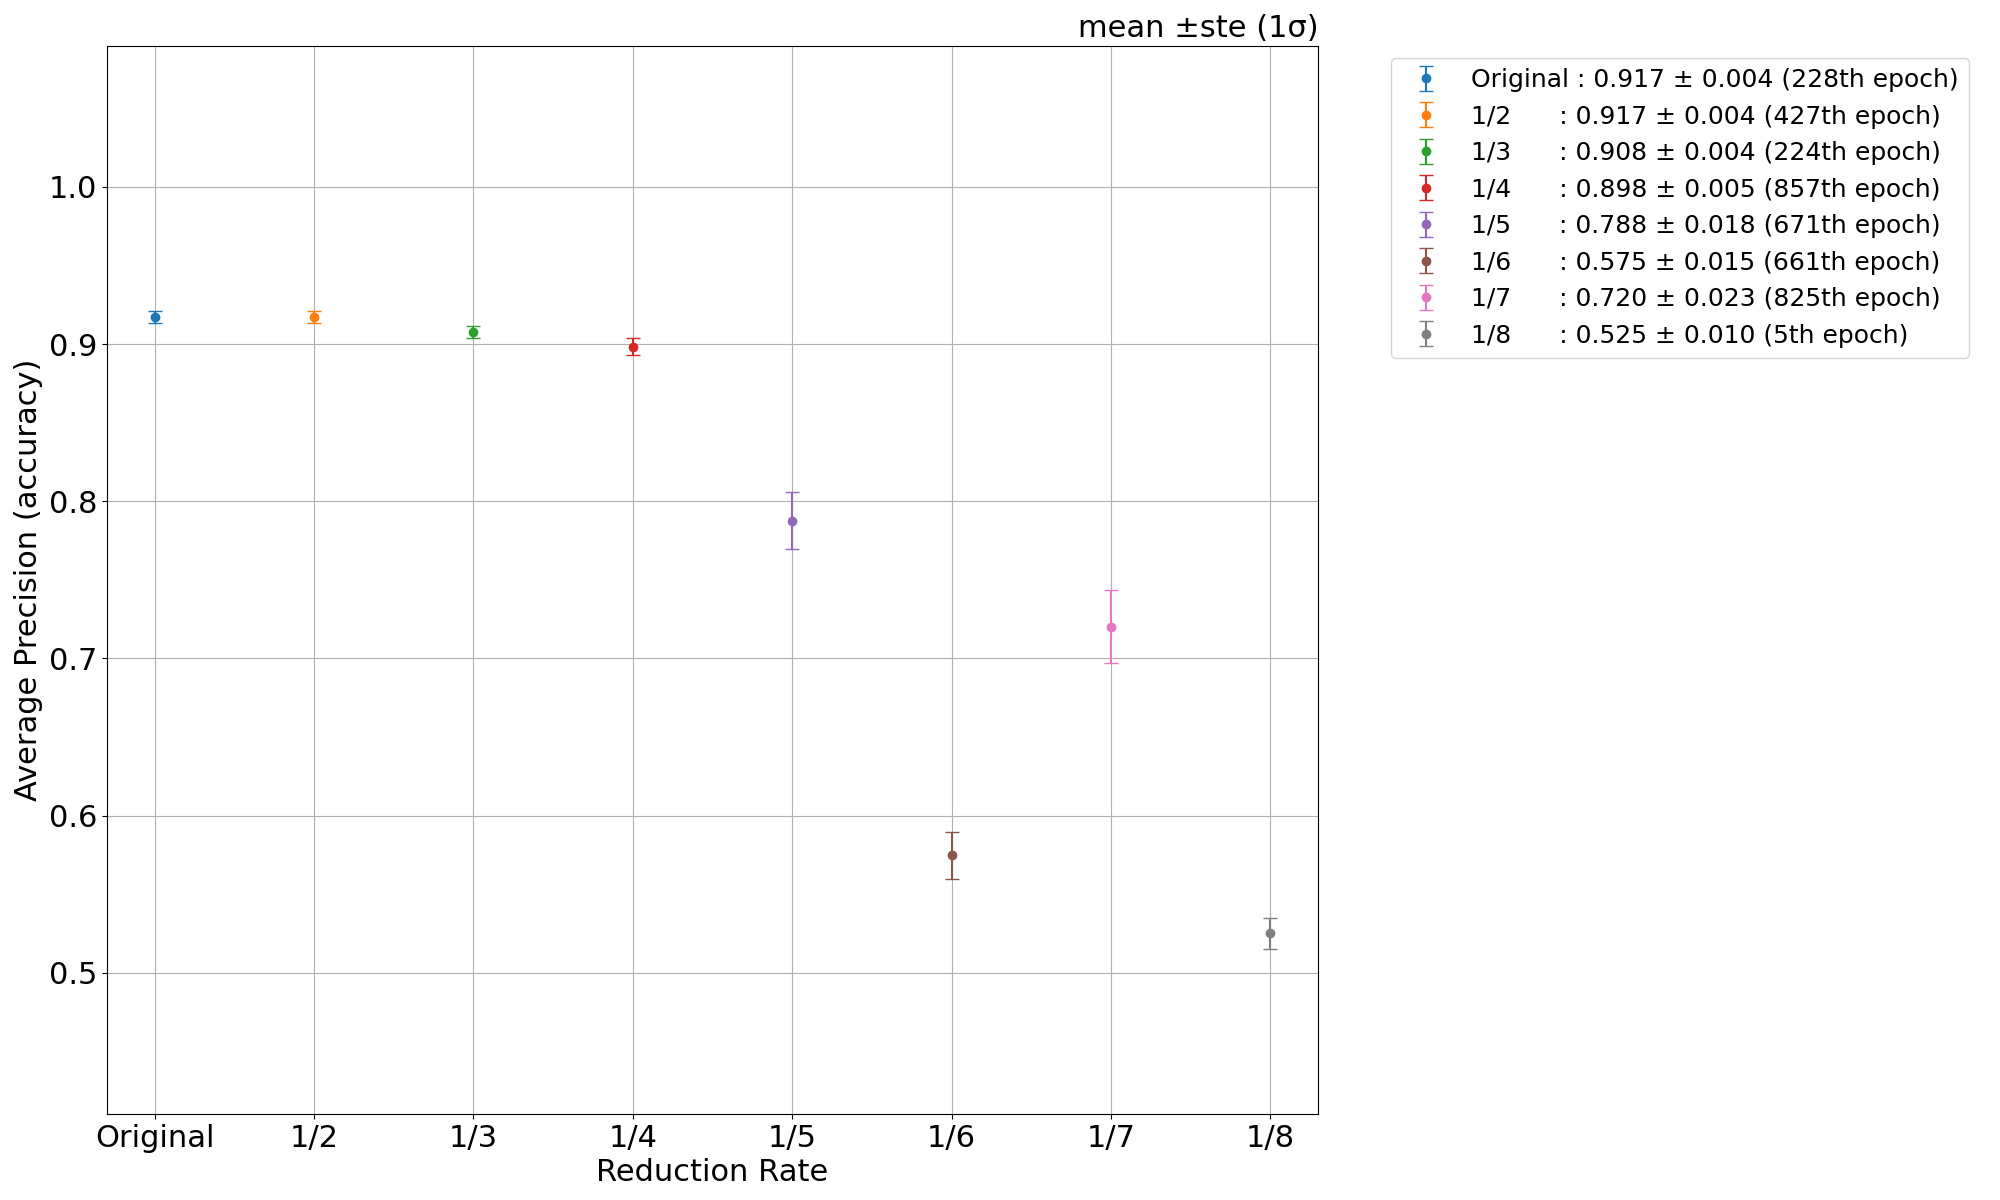
\includegraphics[width=16cm]{images/5syou/print_errorbar/linear/acc_with_errorbar_syuron5_linear_900epoch_30run_300_acc_max_ste1sigma.png}
  \caption{バイリニア補間によって内挿された,縮小データに対するモデルの予測結果(1ste)}
  \label{fig:linear_300_1ste}
\end{figure}
 
\begin{figure}[H]
  \centering
  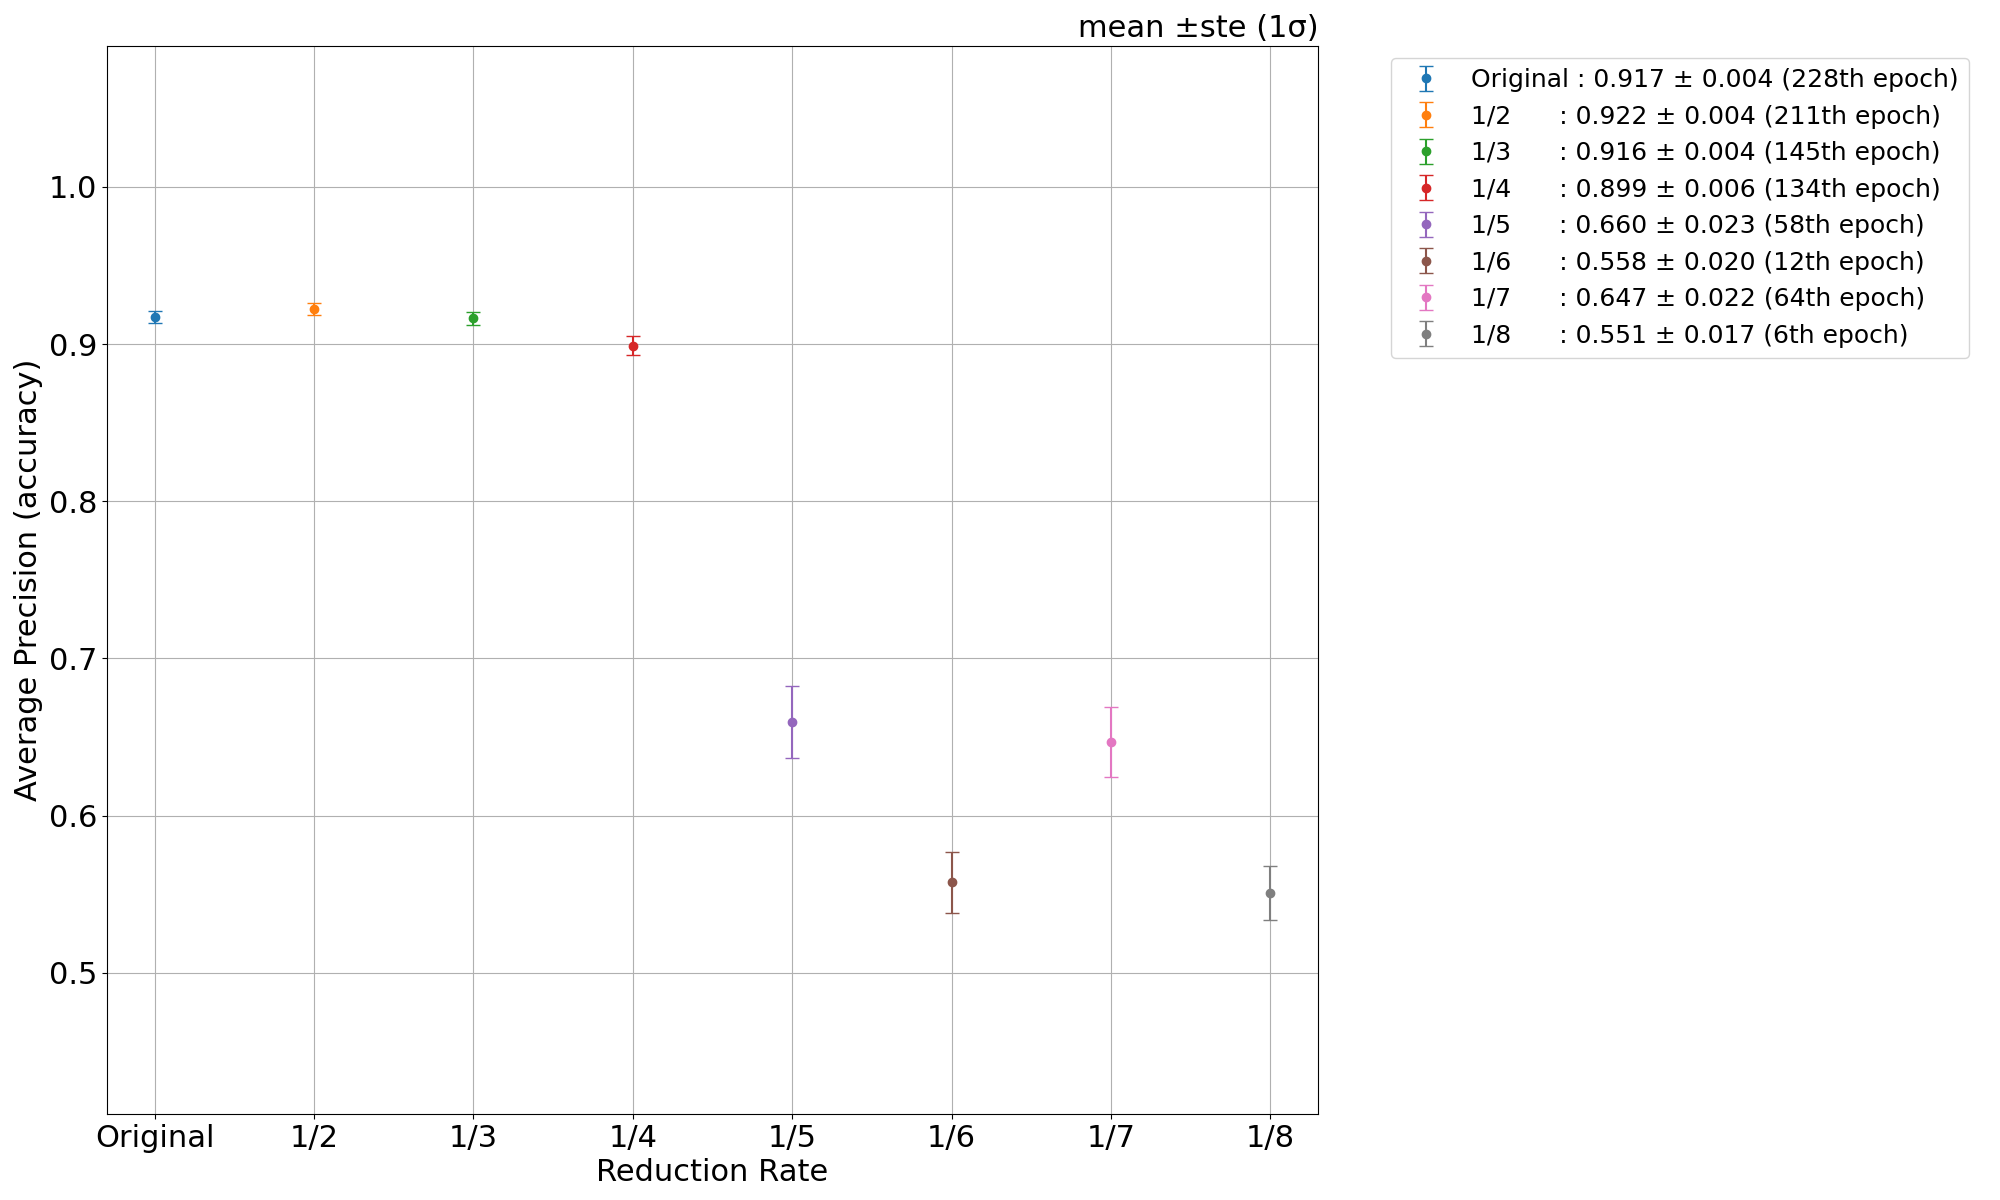
\includegraphics[width=16cm]{images/5syou/print_errorbar/cubic/acc_with_errorbar_syuron5_cubic_900epoch_30run_300_acc_max_ste1sigma.png}
  \caption{バイキュービック補間によって内挿された,縮小データに対するモデルの予測結果(1ste)}
  \label{fig:cubic_300_1ste}
\end{figure}



\newpage
\section{分類精度の使用画像枚数依存性}
当論文で掲げている将来展望として,予測精度を高く保ったまま,学習データの枚数をなるべく少なくする方が好ましい.理由としては,天体画像データセットおよびそれをもとにした形態分類カタログの完成には膨大な時間がかかるからである.

今度登場するであろう高解像度データセットだが,完成には時間がかかる.そのため,完成を待たずある程度の高解像度天体データが撮影された時点で,それらを用い高精度の分類モデルを学習し,既存の低解像度データセットに対し形態分類の予測を適用することが将来展望の構想である.そのため,形態分類の精度を高く保ったまま,どのくらいの使用天体数の少なさなら使えるかを検証することは,将来展望を議論するのに有用である.

これを検証するため,分類精度の使用画像枚数依存性について調べる.具体的には,銀河種ごとの使用天体数をそれぞれ500, 800, 1000天体とし,モデルの学習・テストを行う.5.2節で行っていた300天体の結果も合わせて,使用天体数300, 500, 800, 1000天体で行った実験におけるモデルの予測結果を,テストデータに対する予測のaccuracyをもって比較し,以下を検証する.
\begin{quote}
 \begin{itemize}
  \item テストデータに対する予測のaccuracyの,平均値・誤差(1標準偏差)の増減はあるのか,増減幅はどのくらいか
  \item ''Original''の結果(学習データとテストデータの解像度が揃っている状況での予測結果)と同程度の高精度分類を達成するテストデータの縮小倍率に,変化があるのか
 \end{itemize}
\end{quote}

\subsection{実験条件}
モデルの学習・テストには,GZによる形態分類が行われた15,000天体(図\ref{fig:z_15000}参照)を母集団とし,銀河種類ごとにそれぞれ500,800および1000天体を使用した.銀河種類ごとのデータインバランスが起こらないようにするため,渦巻銀河と楕円銀河の比率は等しくなるように選定をした.選定を行う際,赤方偏移$z$について,$0 < z < 0.2$という条件を設定し,あてはまらない天体は除外を行う.これは,地球との距離が遠すぎる天体については上手く特徴抽出が行えず学習の妨げになる可能性があるからである.

使用天体を選定した後,学習データとテストデータの比率が7:3となるように天体群を分けた.このうち,学習データにはSDSSの切り出し画像,テストデータにはSDSSの切り出し画像を縮小した画像をそれぞれ用いた.また,学習データとテストデータ内において,銀河種のデータインバランスが起こらないようにするため,渦巻銀河と楕円銀河の比率が等しくなるようにした.

モデルの評価を行う際,モデルの学習およびテストを30回行い,accuracyの平均値,標準偏差および標準誤差を導出した.
なお,30回の学習およびテストの際,学習実行毎に使用される天体は毎回シャッフルされる.

モデルの学習期間は900epochとした.これは,すべての縮小データの縮小倍率にて,モデルが学習しきる期間,すなわちテストデータに対するaccuracyが上がりきるepoch数が900epochであったからである.

\subsection{実験結果}
\subsubsection{縮小データに対する予測結果}
銀河切り出し画像を1/2倍から1/8倍に縮小した縮小データに対する,形態分類モデルの予測結果の図を図\ref{fig:nearest_num_of_gal_comparison_1std}から図\ref{fig:cubic_num_of_gal_comparison_1std}に示す.

\begin{quote}
 \begin{itemize}
  \item 横軸が,テストデータである縮小データの縮小倍率であり,縦軸がテストデータに対する予測のaccuracyとなっている.
  \begin{quote}
   \begin{itemize}
    \item テストデータに対する予測のaccuracyについて,30回実行における平均値と標準偏差(2std)をエラーバー形式で示している.
    \item なお,一番左に位置しているOriginalとなっている箇所は,テストデータに縮小データでなく,学習データと同じ大きさの銀河切り出し画像を使用してテストを行った結果である.すなわち,Originalが学習データとテストデータの解像度が揃っている状況での予測結果に対し,1/2から1/8が学習データとテストデータとの間に解像度差がある状況での予測結果を示している.
   \end{itemize}
  \end{quote}
  \item accuracyを採るepoch数は,モデルが十分に学習しきるepoch数とした.すなわち,テストデータに対するaccuracyが最大値となるepoch数とした.
 \end{itemize}
\end{quote}

\begin{figure}[H]
  \centering
  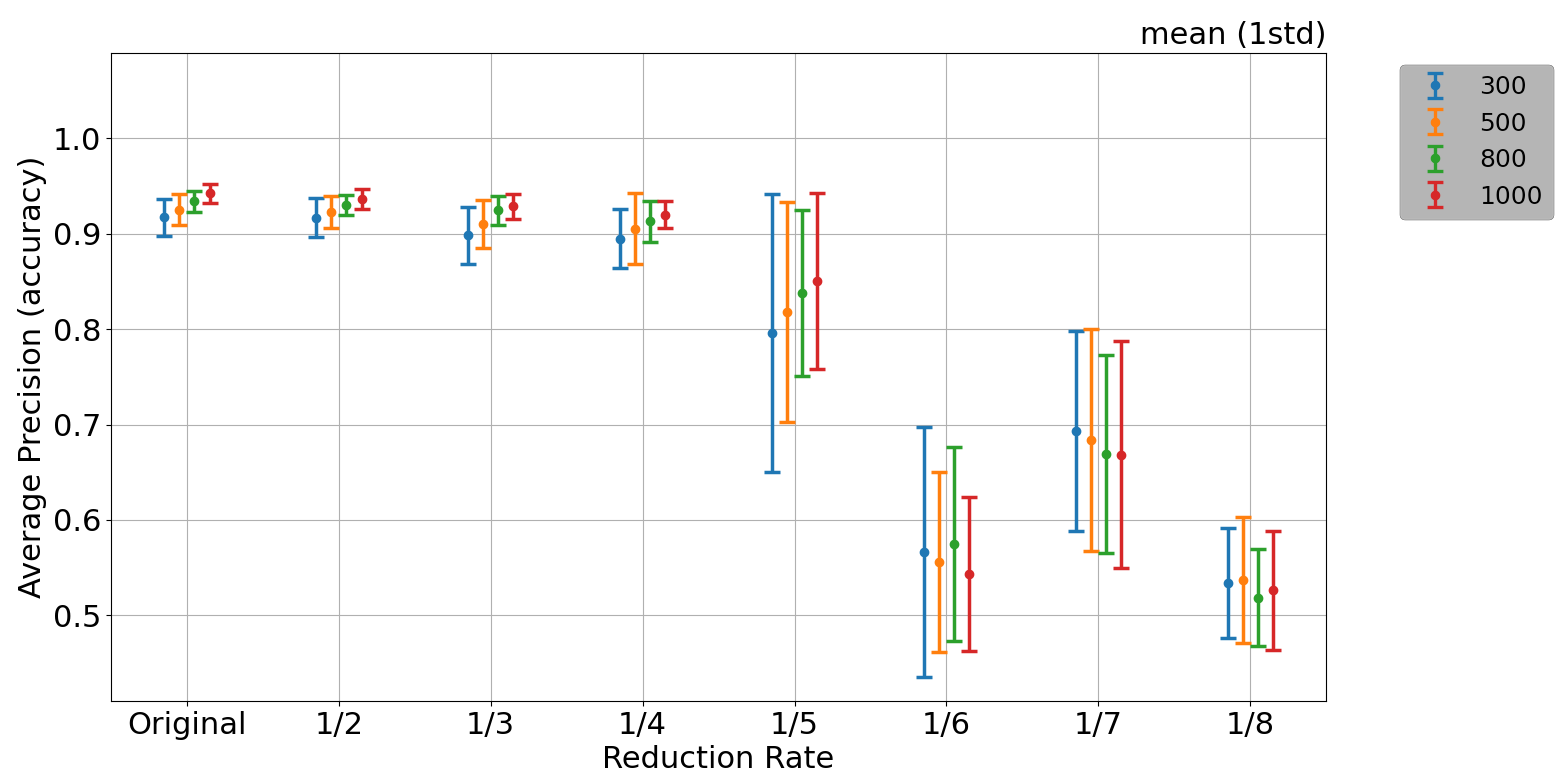
\includegraphics[width=1.0\hsize, keepaspectratio]{images/5syou/print_errorbar/nearest/acc_with_errorbar_syuron5_nearest_900epoch_30run_num_of_gal_comparison_acc_max_std1sigma.png}
  \caption{最近傍補間によって内挿された,縮小データに対するモデルの予測結果(1std)}
  \label{fig:nearest_num_of_gal_comparison_1std}
\end{figure}

\begin{figure}[H]
  \centering
  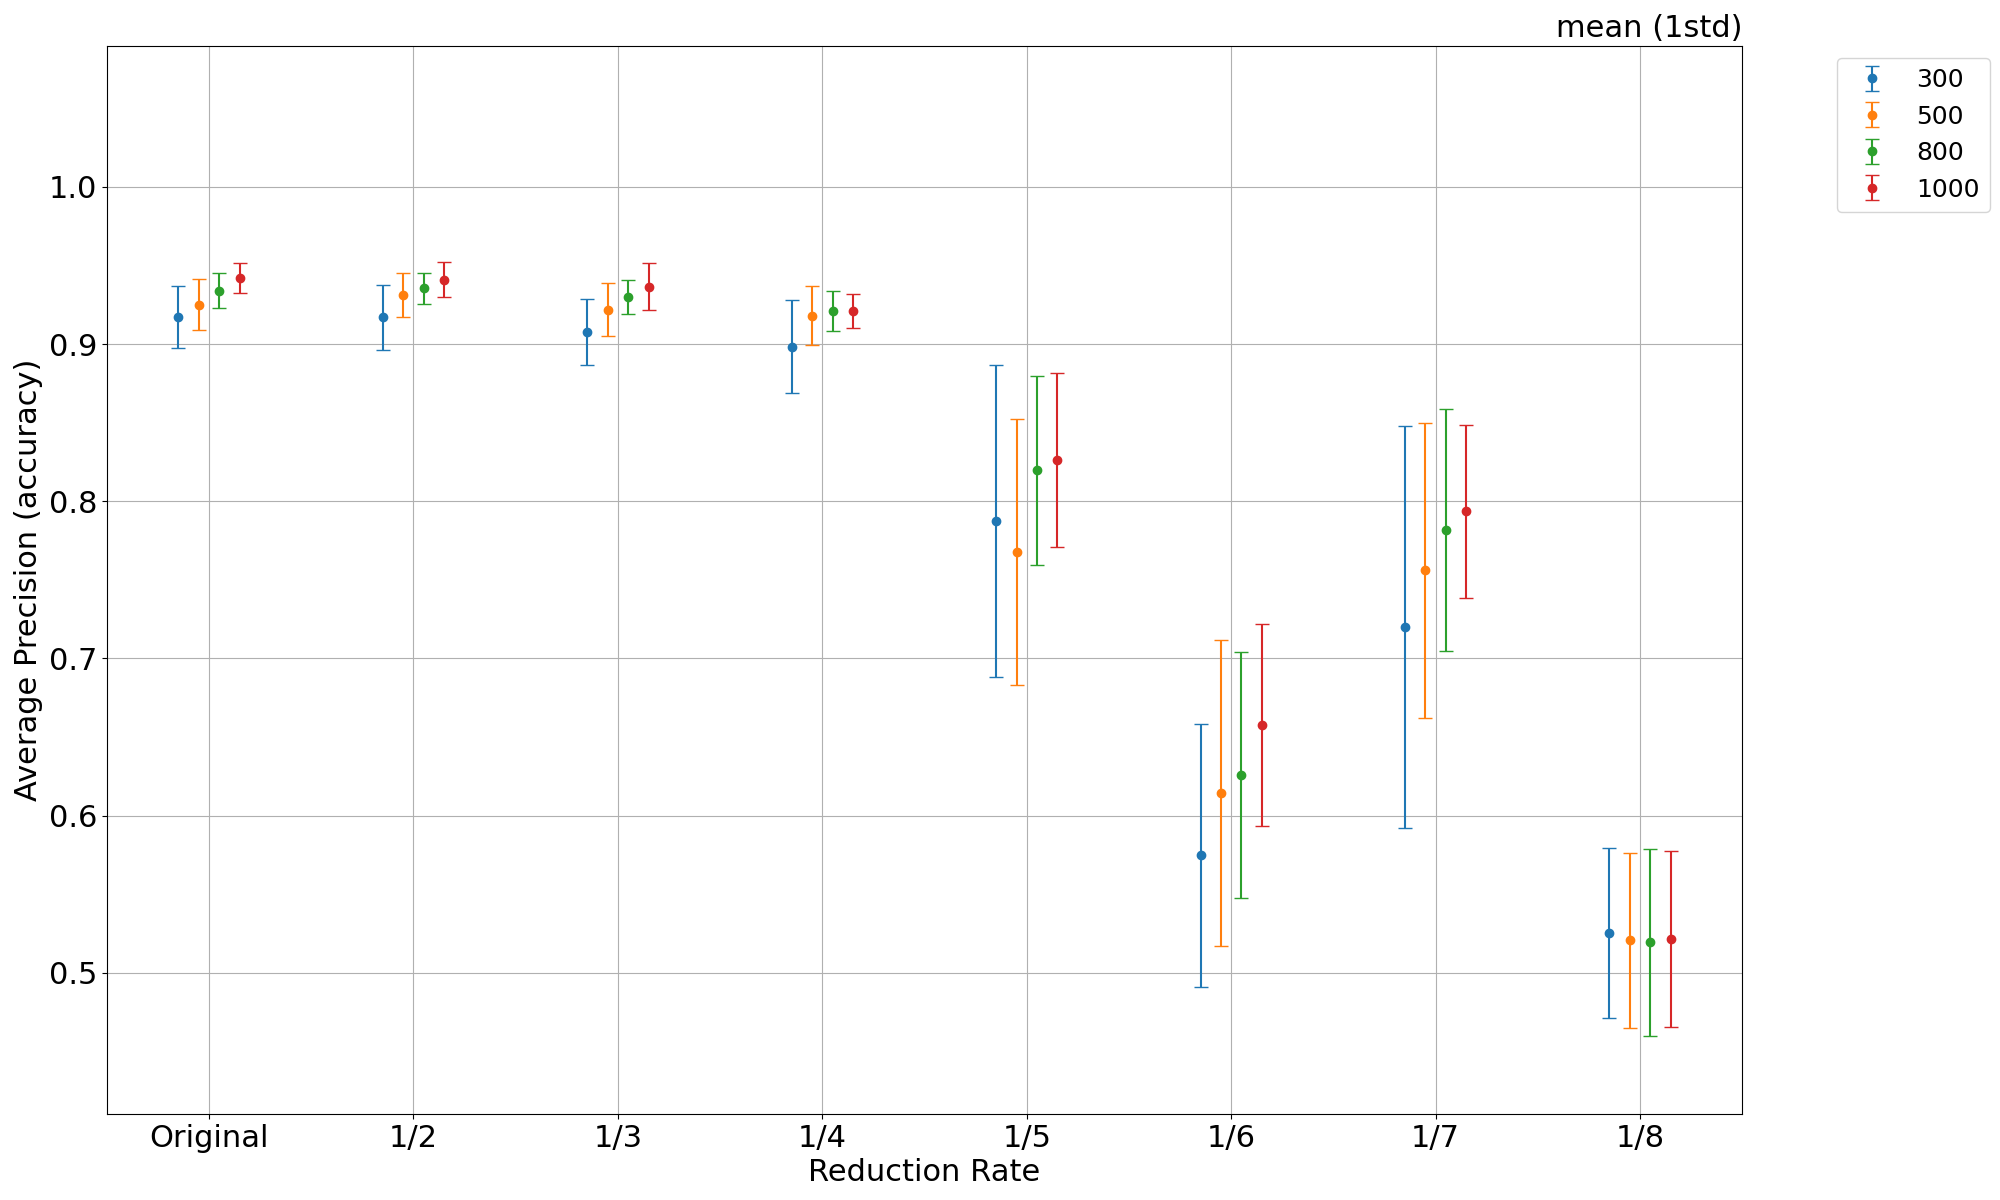
\includegraphics[width=1.0\hsize, keepaspectratio]{images/5syou/print_errorbar/linear/acc_with_errorbar_syuron5_linear_900epoch_30run_num_of_gal_comparison_acc_max_std1sigma.png}
  \caption{バイリニア補間によって内挿された,縮小データに対するモデルの予測結果(1std)}
  \label{fig:linear_num_of_gal_comparison_1std}
\end{figure}

\begin{figure}[H]
  \centering
  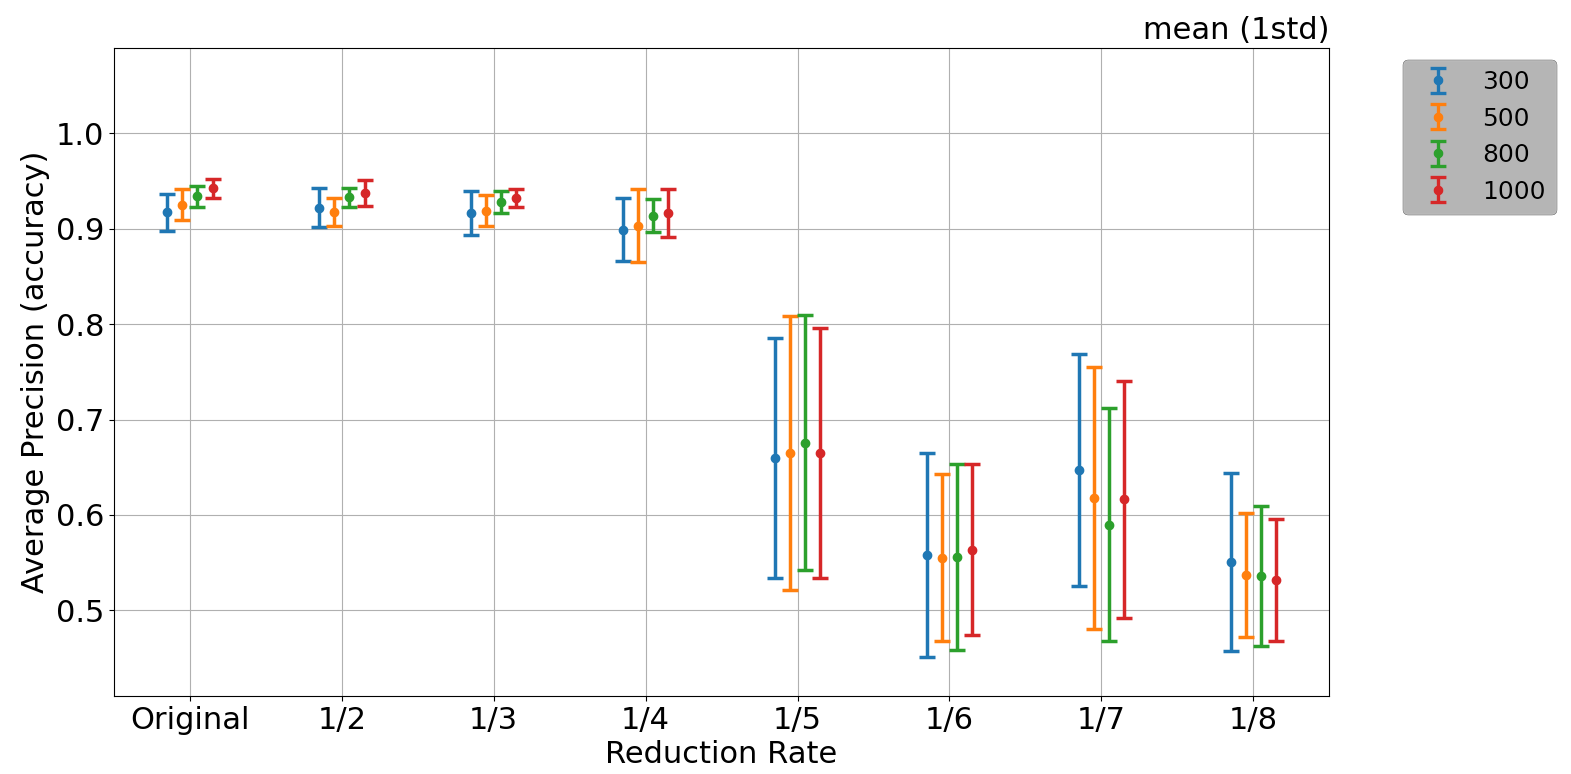
\includegraphics[width=1.0\hsize, keepaspectratio]{images/5syou/print_errorbar/cubic/acc_with_errorbar_syuron5_cubic_900epoch_30run_num_of_gal_comparison_acc_max_std1sigma.png}
  \caption{バイキュービック補間によって内挿された,縮小データに対するモデルの予測結果(1std)}
  \label{fig:cubic_num_of_gal_comparison_1std}
\end{figure}

\subsubsection{結果}
\paragraph{使用天体数増加によるaccuracyの変化}
使用天体数を増やすことで補間方法によらず,縮小倍率が1/2倍から1/4倍の縮小画像データに対する予測のaccuracyの平均値が上昇し,また標準偏差の値も小さくなった.特に使用枚数が300枚と1000枚の結果を比較すると,標準偏差の値がおよそ半減していることが図\ref{fig:nearest_num_of_gal_comparison_1std}から図\ref{fig:cubic_num_of_gal_comparison_1std}より読み取れる.

また縮小倍率が1/5倍から1/8倍に対する予測のaccuracyについては,内挿方法によりaccuracyの挙動に差が出た.これについては\textbf{内挿方法間での比較}にて詳述する.


\paragraph{内挿方法間での比較}
内挿方法の間で,銀河種ごとの天体使用数を増加させた際に見受けられる,テストデータに対するaccuracyの細かい挙動を比較する.なお,縮小倍率1/2倍から1/4倍のデータに対する予測結果は前段落である\textbf{使用天体数増加によるaccuracyの変化}で述べたので,ここからは縮小倍率が1/5倍以上のデータに対する結果を比較する.

最近傍補間によってテストデータの内挿を行った場合,銀河種ごとの天体使用数を増加させることで,縮小倍率1/5倍のデータに対する予測のaccuracyの平均値上昇,および標準偏差の減少が見受けられる.しかしながら,標準偏差の減少量は1/2倍から1/4倍の縮小倍率データに対する予測と比べるとそれほど大きくないことが分かる.

バイリニア補間によってテストデータの内挿を行った場合,銀河種ごとの天体使用数を1000天体まで増やしても,1/5倍から1/8倍の縮小倍率データに対する予測のaccuracyが0.9を超えず,高精度分類を行えなかった.しかしながら,銀河種ごとの天体使用数を増加させることで,縮小倍率が1/5倍から1/7倍のテストデータに対する予測のaccuracyの精度改善が見込めた.
\\なお1/8倍の縮小倍率に対する形態分類は,銀河種ごとの天体使用数および内挿方法を問わずaccuracy0.5付近を記録した.このため,学習データとテストデータとの間の解像度差が1/8倍である場合,深層学習モデルによる形態予測が行えないのではないかと思われる.

バイキュービック補間によってテストデータの内挿を行った場合,銀河種ごとの天体使用数を1000天体まで増やしても,1/5倍から1/8倍の縮小倍率データに対する予測のaccuracyが0.9を超えず,またaccuracyの平均値および標準偏差に改善が見られなかった.

\paragraph{使用可能なデータセット間の解像度差について}
図\ref{fig:nearest_num_of_gal_comparison_1std}から図\ref{fig:cubic_num_of_gal_comparison_1std}より,内挿方法を問わず,銀河種ごとの天体使用数が何天体であっても,縮小倍率が1/4倍までの縮小データに対する予測のaccuracyが,Originalの結果(学習データとテストデータの解像度が揃っている状況での予測結果)と同程度かつaccuracyが0.9付近を記録することが読み取れる.このことから,内挿方法・銀河種ごとの使用天体数によらず,学習データとテストデータの解像度差が1/4までならば使用可能であることが分かった.
\\また\textbf{内挿方法間での比較}にて,縮小倍率が1/4倍までの縮小データに対する予測では,銀河種ごとの天体使用数を増加させることで内挿方法によらず予測精度が向上することが分かった.このことから,学習データとテストデータの解像度差が1/2倍から1/4倍ほどである2値銀河形態分類は,モデルの学習の上振れを期待せずとも,高精度の形態予測を期待できる分類問題であると思われる.

次に,学習データとテストデータの解像度差が1/5倍より大きい場合について述べる.最近傍補間によってテストデータを内挿する場合,解像度差が1/5倍のとき,銀河種ごとの天体使用数を増やすことで誤差区間が減少する.しかし,最も多い天体数である使用天体数1000天体においても,1標準偏差区間の上位25\%しかaccuracyが0.9を超えず,このことから,モデルの学習が上振れることを期待する必要があるため使用不可な解像度差であると判断した.
\\また,図\ref{fig:linear_num_of_gal_comparison_1std},図\ref{fig:cubic_num_of_gal_comparison_1std}より,バイリニア補間,およびバイキュービック補間においては,Originalの結果と同程度かつaccuracyが0.9付近を記録しないことが読み取れる.

したがって,学習データとの解像度差が1/5倍より大きいテストデータは使用不可であることがわかった.
\section{5章全体の議論・結論}
\subsubsection{どの補間フィルタを用いるべきか}
第5章では学習データに高解像度,テストデータに低解像度の画像データを使用していた.深層学習モデルに入力する画像データは全て同じサイズである必要があるため,今回の実験ではテストデータである低解像度画像を拡大を行った.\\ここで,今回の画像拡大に用いた3手法(最近傍補間・バイリニア補間・バイキュービック補間)のうち,どれを使うべきかを考察する.

まず,第5章にて''使用可能''と定義した,学習データとテストデータとの間の解像度差が1/2倍から1/4倍の状況でモデルの学習・それによる予測を行う場合について考察する.図\ref{fig:nearest_num_of_gal_comparison_1std}から図\ref{fig:cubic_num_of_gal_comparison_1std}より,どの天体使用数においても,3つの拡大手法でのaccuracyは同程度の挙動,なおかつ0.9付近のスコアを記録している.このことから,学習データとテストデータとの間の解像度差が1/2倍から1/4倍の状況でモデルの学習・それによる予測を行う場合,これら3手法のどれを使用しても高精度の予測が行えると考えられる.
\\ただし図\ref{fig:cubic_num_of_gal_comparison_1std}より,バイキュービック補間は使用天体数を増やした際のaccuracy平均値向上・誤差低下の恩恵を受けづらいことが読み取れる.

次に,第5章にて''使用不可''と定義した,学習データとテストデータとの間の解像度差が1/5倍から1/8倍の状況でモデルの学習・それによる予測を行う場合について考察する.この場合,5.3.2の結果における\textbf{内挿方法間での比較}より,使用天体数を増加させた際のaccuracy平均値向上・誤差低下が最も見込めるバイリニア補間が適していると思われる.

最後に,3つの拡大手法の処理にかかる時間を考える.時間計測を行うため,SDSSから取得した銀河切り出し画像を1/8倍に縮小した縮小画像を,GZの分類ラベルにてラベル付けされた渦巻銀河50天体・楕円銀河50天体について拡大処理を実行した.拡大処理は各手法にてそれぞれ10000回ずつを7周実行し,拡大にかかった時間の平均値および1標準偏差を導出した.
\\表\ref{tb:calc_cost_by_interpolation}に3つの拡大手法の処理にかかる時間を示す.表より,最近傍補間が最も処理が軽く,バイリニア補間が2番目,バイキュービック補間が3番目に処理に時間がかかることが読み取れる.

上で述べた3つを総合的に考慮すると,モデルの学習・テストにおける処理を最も軽くしたい場合は最近傍補間が望ましいと考えられる.
\\また処理が少し重くてもよく,使用天体数を多くした際のaccuracyに対する恩恵を受けたい場合はバイリニア補間による内挿がよいと思われる.
\\バイキュービック補間は,使用天体数を増加させた際のaccuracyに対する恩恵を最も受けづらく,また拡大処理における処理の重さを考えると,3手法の中では使用する意味が最も薄いと考えられる.

\begin{table}[htbp]
  \centering
	\caption{各補間フィルタによる拡大の計算コスト(平均値(1標準偏差))}
  \begin{tabular}{|c|c|}
		\hline
    最近傍補間 & $247\mu s \pm 2.25\mu s$ \\ \hline
    バイリニア補間 & $378\mu s \pm 5.37\mu s$ \\ \hline
    バイキュービック補間 & $1.48ms \pm 7.74\mu s$ \\ \hline
  \end{tabular}
  \label{tb:calc_cost_by_interpolation}
\end{table}

\subsubsection{学習データとテストデータとの間の解像度差が1/6および1/7の際の,テストデータに対する予測accuracyの挙動}
第5章にて使用天体数・内挿方法を問わず共通の傾向であった,「縮小倍率が1/7倍の縮小データに対する予測精度が,縮小倍率1/6倍の予測精度より高い」事に対し,考察を行う.

一般的に,テストデータの解像度が低ければ低いほど,分類モデルによる予測精度は低くなると考えられる.図\ref{fig:nearest_num_of_gal_comparison_1std}から図\ref{fig:cubic_num_of_gal_comparison_1std}においても,縮小倍率が1/2倍から1/6倍においては上記の傾向が見受けられる.しかしながら,1/7倍の縮小倍率に対する予測精度は,1/2倍から1/6倍にて見受けられた傾向から逸脱している.この傾向に対し,考察を行う.

1/6倍, 1/7倍の縮小画像に対する画像拡大例を図\ref{fig:1_6and1_7}に示す.図\ref{fig:1_6and1_7}より,拡大手法によって生成される画像が,見かけではかなり異なることが分かる.しかし,図\ref{fig:nearest_num_of_gal_comparison_1std},図\ref{fig:linear_num_of_gal_comparison_1std}を比較すると,拡大手法によって縮小倍率1/6倍と縮小倍率1/7倍のaccuracyの挙動に大きな差はないことが分かる.ここで,1/6倍,1/7倍の縮小画像(図\ref{fig:1_6and1_7}の左下)を見ると,画像内の最も明るいピクセルが存在する場所に差があることが分かる.1/6倍の縮小画像では中央より右下,1/7倍の縮小画像では中央が一番明るいピクセルであることが読み取れる.このことから,平均画素法による縮小の際,何らかの形で銀河の形態的特徴が損失している可能性がある.そしてこの形態的特徴損失により,学習データとテストデータとの間の解像度差が1/6および1/7の際の,テストデータに対する予測accuracyの挙動に影響を及ぼしていると思われる.

\begin{figure}[htbp]
 \centering
 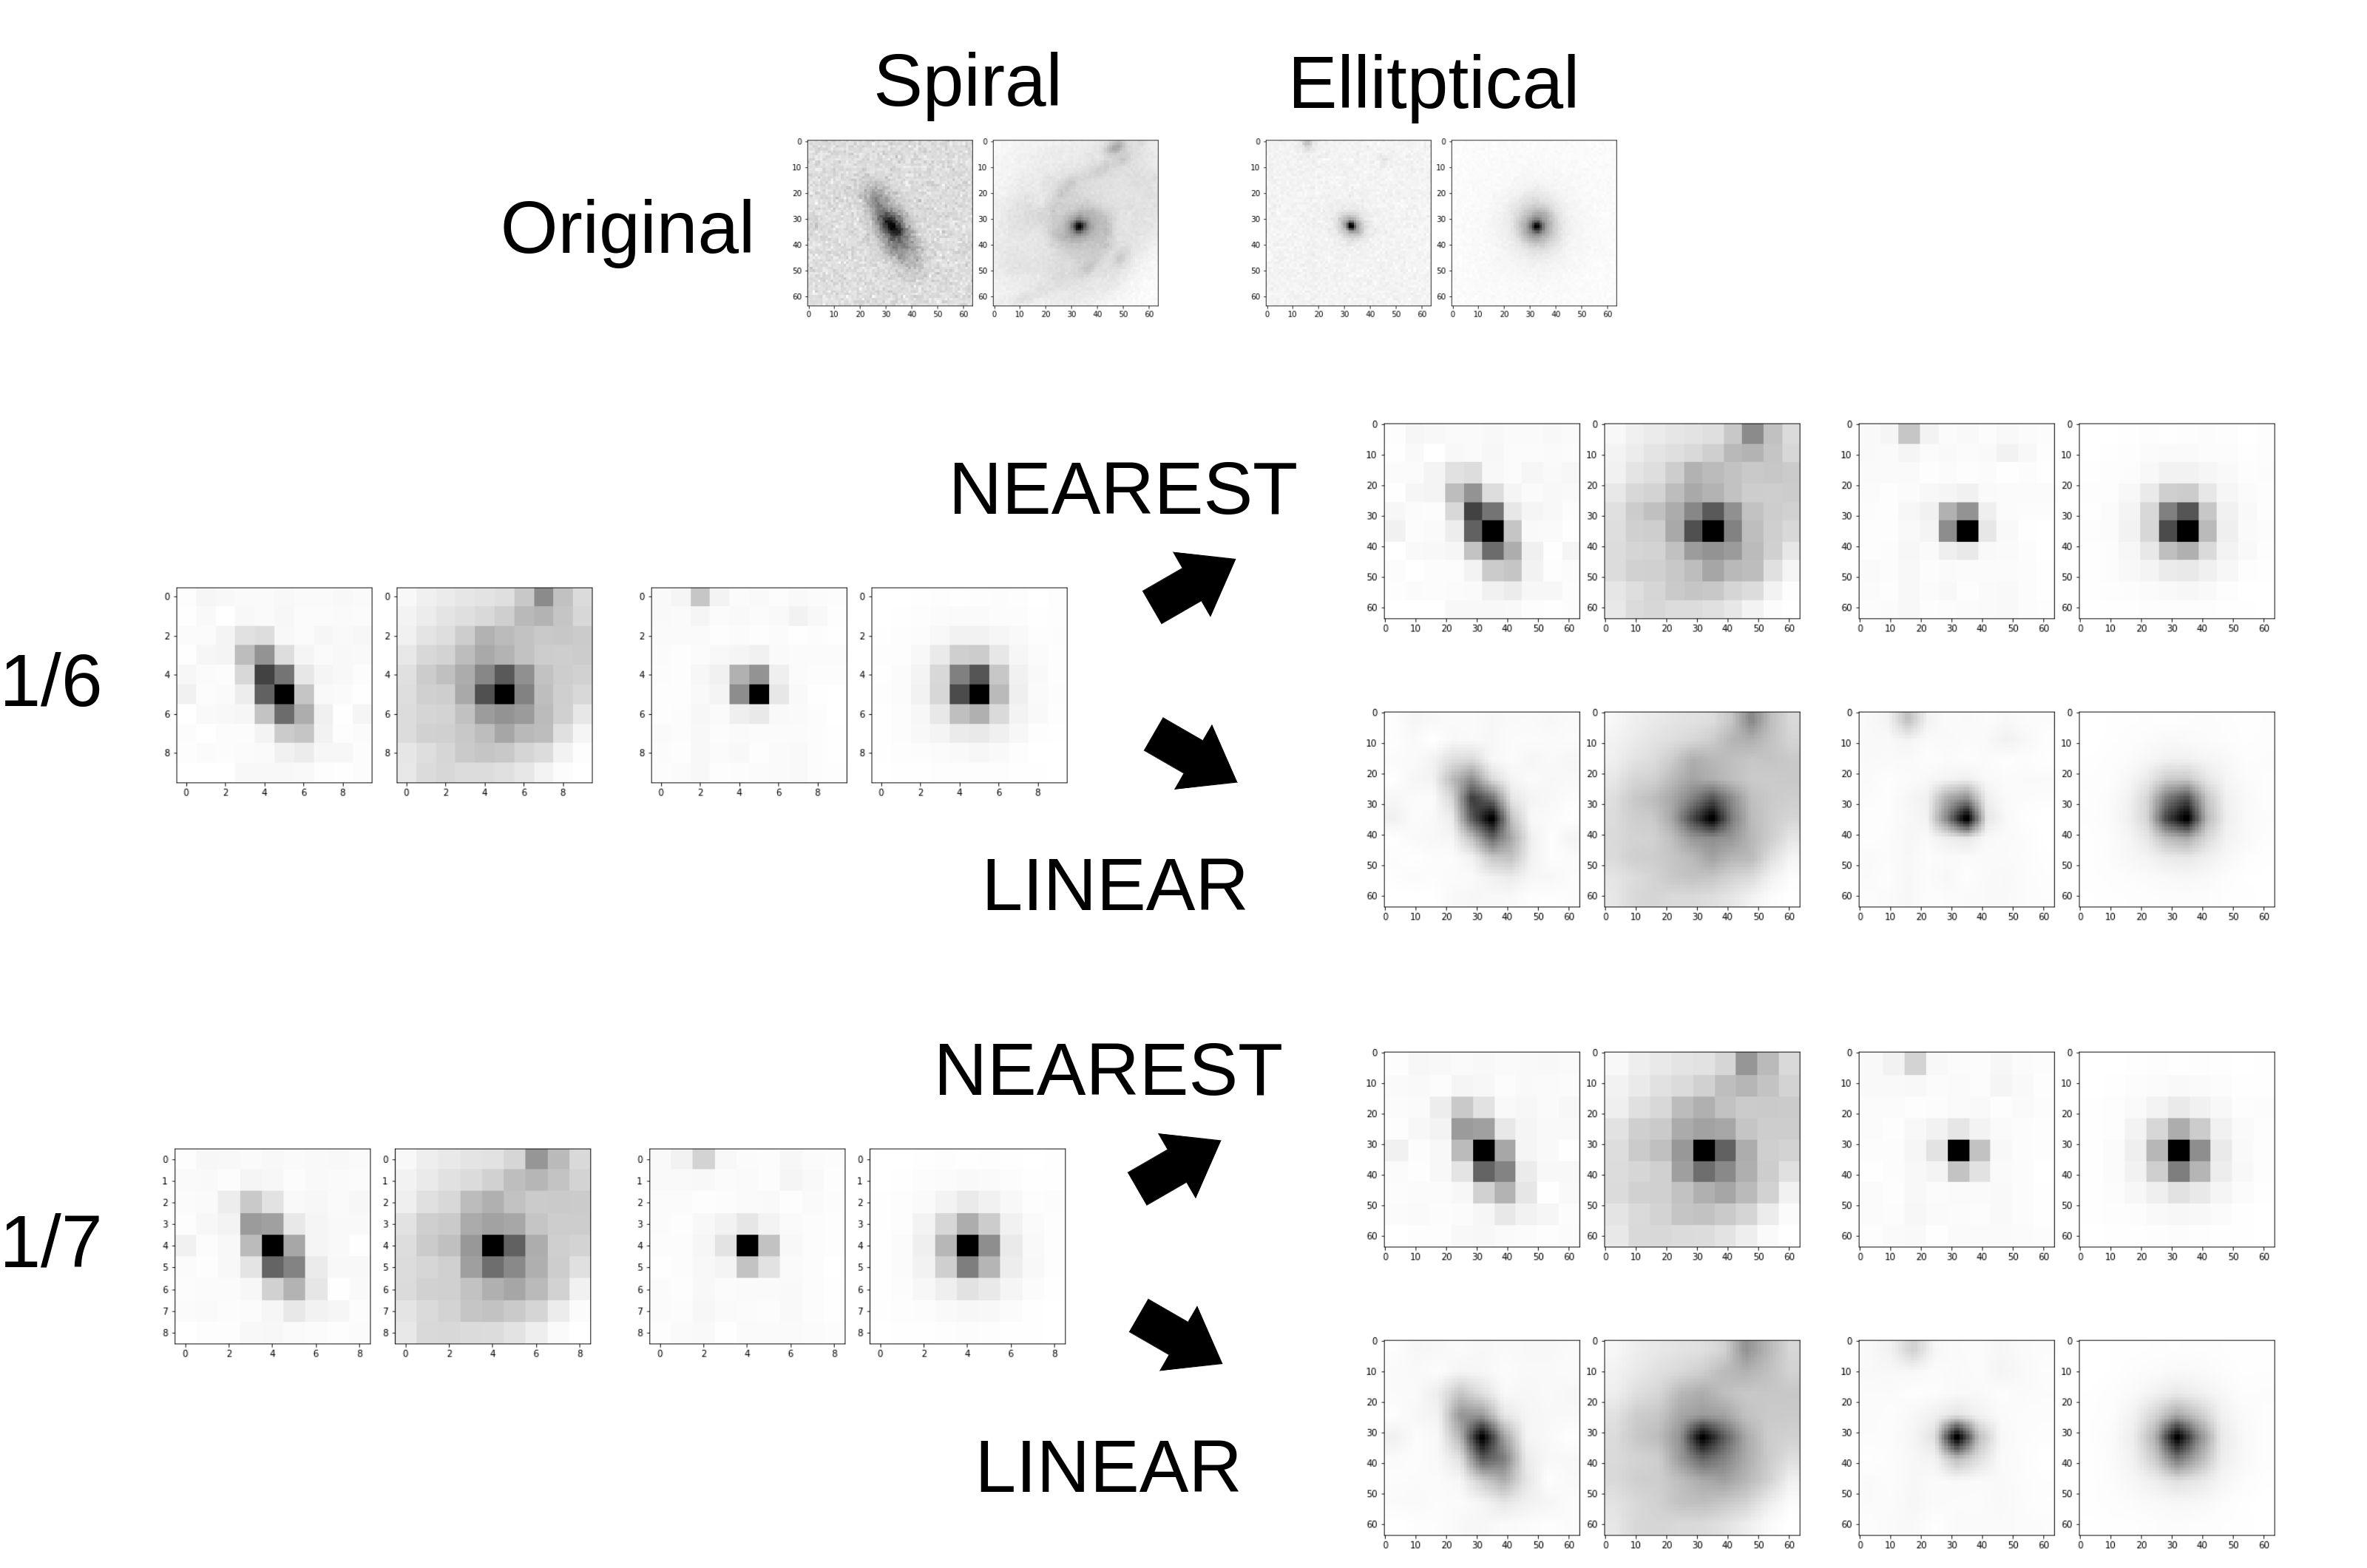
\includegraphics[width=1.0\hsize, keepaspectratio]{images/5syou/syuron_5syou_kakudai/ver1/5syou_giron_1_6and1_7.png}
 \caption{1/6倍, 1/7倍の縮小画像に対する画像拡大例(最近傍補間・バイリニア補間)}
 \label{fig:1_6and1_7}
\end{figure}


\subsubsection{使用枚数が何枚までならば高精度を保てるか}
最後に,モデルの学習・テストに用いる銀河種ごとの天体使用数について,形態分類の精度を高く保ったまま,どのくらいの使用天体数の少なさなら''使用可能''かについて議論を行う.なお,第5章全体を通して''使用可能''と定義している学習データとテストデータとの間の解像度差が1/2倍から1/4倍の状況に限定して,使用天体数の議論を行う.

図\ref{fig:nearest_num_of_gal_comparison_1std}から図\ref{fig:nearest_num_of_gal_comparison_1std}より,使用する天体数は何天体でもよいと思われる.これは,内挿方法を問わず,''Original''と同程度の予測精度,すなわちaccuracyが0.9程度をスコアするからである.ここでテストデータに対する予測のaccuracyを0.9以上にしたい場合だが,図\ref{fig:nearest_num_of_gal_comparison_1std}から図\ref{fig:nearest_num_of_gal_comparison_1std}より,これは銀河種ごとの天体使用数を800天体以上にすることが望ましいと考えられる.

この章では,「学習データとテストデータとの間の解像度差がある状況において,分類モデルの学習が行えるか」の検証を行うため,2つの実験を行った.

学習データとテストデータとの間の解像度差が1/4までならば,内挿方法によらず使用可能,すなわち学習データとテストデータの解像度が揃っている状況での予測結果である”Original” と同程度の高精度な分類,すなわちaccuracy が0.9 付近を記録する結果となった.

銀河種ごとの使用天体数を増加させた際,テストデータに対する予測のaccuracyの挙動は内挿方法によって差が生じた.最近傍補間による内挿では,1/2倍から1/5倍までの縮小倍率画像に対し精度改善が見込めた.バイリニア補間に関しては,1/2倍から1/7倍までの縮小倍率画像に対し精度改善が見込めた.バイキュービック補間は1/2倍から1/4倍までの縮小倍率ならば精度改善が見込めたが,他2手法よりもその恩恵は小さく,更に1/5倍より大きい縮小倍率画像に対する予測精度は改善が見込めなかった.

内挿方法によってテストデータに対する予測精度が異なる挙動を見せることから,モデルへの内挿方法を模索することで,更なる精度改善,および当論文では使用不可と判断した学習データとテストデータとの間の解像度差においても,高精度分類が行える可能性がある.

\newpage
\chapter{議論}
\section{今回の実験から得た結論}
当論文の将来展望は,高空間分解能観測装置データを用いてモデル学習を行うことで,既存の低空間分解能データセットに対し更なる高精度形態分類を提供するというものである.この将来展望が実現できる可能性を検証するため,当論文では第4章,第5章にて将来展望の前段階となる実験群を行った.その結果,深層学習による銀河形態分類の主に渦巻銀河・楕円銀河に分類する2値分類問題において,学習データとテストデータとの間に1/4倍の画像解像度差が生じていても,テストデータに対しaccuracyが0.9付近となる高精度分類が提供できることが分かった.このことから,将来展望である「異なる観測装置データの組み合わせを行い,深層学習による銀河形態分類」を実現できる可能性が示された.

一方で,SDSS DR7とGZ1を組み合わせた深層学習による形態分類の更なる精度向上など,多くの将来課題が残されている.6.2節ではそれらについて言及を行う.

\section{将来課題}
\subsubsection{学習した分類モデルの精度のよさについて}
モデルの分類精度を向上するべきである.\\
将来展望(ポンチ絵)は,「高$\to$低」が「低$\to$低」を上回る.\\
(その際,「高$\to$低」は「高$\to$高」レベルの分類精度であることが望ましい.)\\
それはモデルを学習させるデータがより細かい特徴を持った高解像度画像だからって理由.\\

しかし,現状では「低$\to$低」の組み合わせでも割と分類でき,「高$\to$低」に匹敵する分類精度を持っている.\\
「低$\to$低」で割と行けるなら,「高$\to$低」や「高$\to$高」でももっと行けるはず.\\

精度向上案\\
GZの論文(どれか忘れた)やcheng+(2019)より,「いろんな色を組み合わせると,形態的特徴が増える」\\
$\to$用いるband数増やしてみる\\
モデルのハイパパラメータチューニングを行う.\\
今回のモデルはSDSSの解像度など,今回の実験条件に最適化されておらず,モデルのチューニングを行うことで精度向上が見込める可能性がある.\\

\subsubsection{実際に未知天体データセット(ラベル付けが為されていないデータセット)に用いる時の方法}
どうやって最高のモデルを残すの?\\
$\to$今回みたいに○○回実行したあと,その地点までのモデルをk分割交差検証法?\\
何個もモデル作って未知天体に適用.一番多いラベルを予測結果とする という使用方法\\

\subsubsection{GZ1の不確かを,深層学習でどう扱うか}
・今回はGZ1の不確かについて注目しているが,他にも人間の目による分類がまだ提供されていないデータセット(ex. HSCの銀河データセット)に対し先んじて提供,等の使い道があるかもしれない\\
教師なし学習利用\\
GZ1の分類(人間の目による分類)と比較して,教師なし学習による分類がどれくらい信頼できるかを調べれば,GZ1に不確かと分類された天体に渦巻銀河・楕円銀河の2値分類を提供できるかもしれない


\section{将来展望}
当論文にて異なる観測装置データの組み合わせによる深層学習形態分類の可能性が示された.そこで,ここからは実際に異なる観測装置データの組み合わせを行った結果を示す.
\subsection{実験概要}
学習データである高解像度データセットとして,HSCから取得した銀河切り出し画像を用いた.ここで,HSCとは...(HSCの説明)

学習データの正解ラベルだが,これはHSCの銀河画像を人間の目による分類を行った分類ラベルが存在しなかったため,GZ1による分類ラベルを流用した.

テストデータである低解像度データセットとして,第4,5章にて用いてきたSDSSから取得した銀河切り出し画像を使用した.ここで,HSCの空間分解能が0.168''/pix,SDSSの空間分解能は0.369''/pixであり,これらの分解能の差はおよそ2.3倍である.これは第5章にて結論付けた''使用可能''である解像度差の範囲内である.

モデルの学習・テストに使用する天体数として,銀河種ごとに1000天体ずつを使用した.選定された天体は,学習データとテストデータの比率が7:3となるように振り分けられた.なお,学習データおよびテストデータ内における渦巻銀河と楕円銀河の比率は等しくなるようにした.取得を行う際,赤方偏移$z$について,$0 < z < 0.2$という条件を設定し,あてはまらない天体は除外を行う.これは,地球との距離が遠すぎる天体については上手く特徴抽出が行えず学習の妨げになる可能性があるからである.

今回用いた深層学習モデルは,cheng et al.(2019)\ref{Cheng2019}にて用いられていた銀河形態分類モデルを参考にした.今回用いたモデルの構造を図\ref{fig:model_shape_3}に示す.このモデルは畳み込み層を合計3つ有しており,それぞれのカーネルサイズは3x3, 3x3, 2x2である.それぞれの畳み込み層の後には,2x2のmax-pooling層が存在する.全畳み込み層の後に全結合層が2層配置されており,それぞれ1024個のノードを有している.

モデルの評価を行う際,モデルの学習およびテストを30回行い,accuracyの平均値,標準偏差および標準誤差を導出した.なお,30回の学習およびテストの際,学習実行毎に取得される天体は毎回シャッフルされる.

\begin{figure}[h]
	\centering
	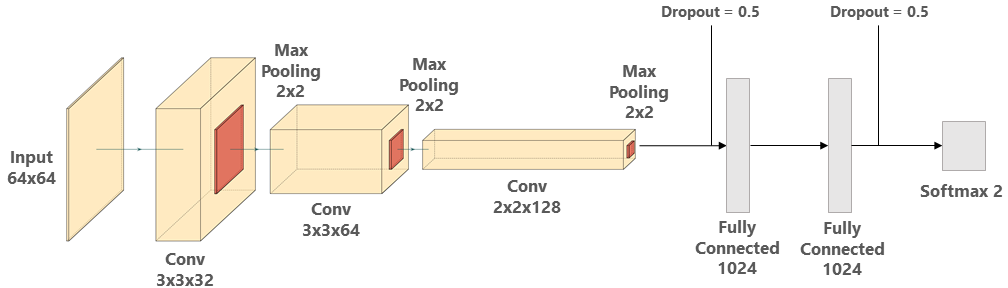
\includegraphics[width=14cm]{images/model_shape.png}
	\caption{用いた分類モデルの構造図}
	\label{fig:model_shape_3}
\end{figure}

\subsection{実験結果}

\begin{figure}[H]
  \centering
  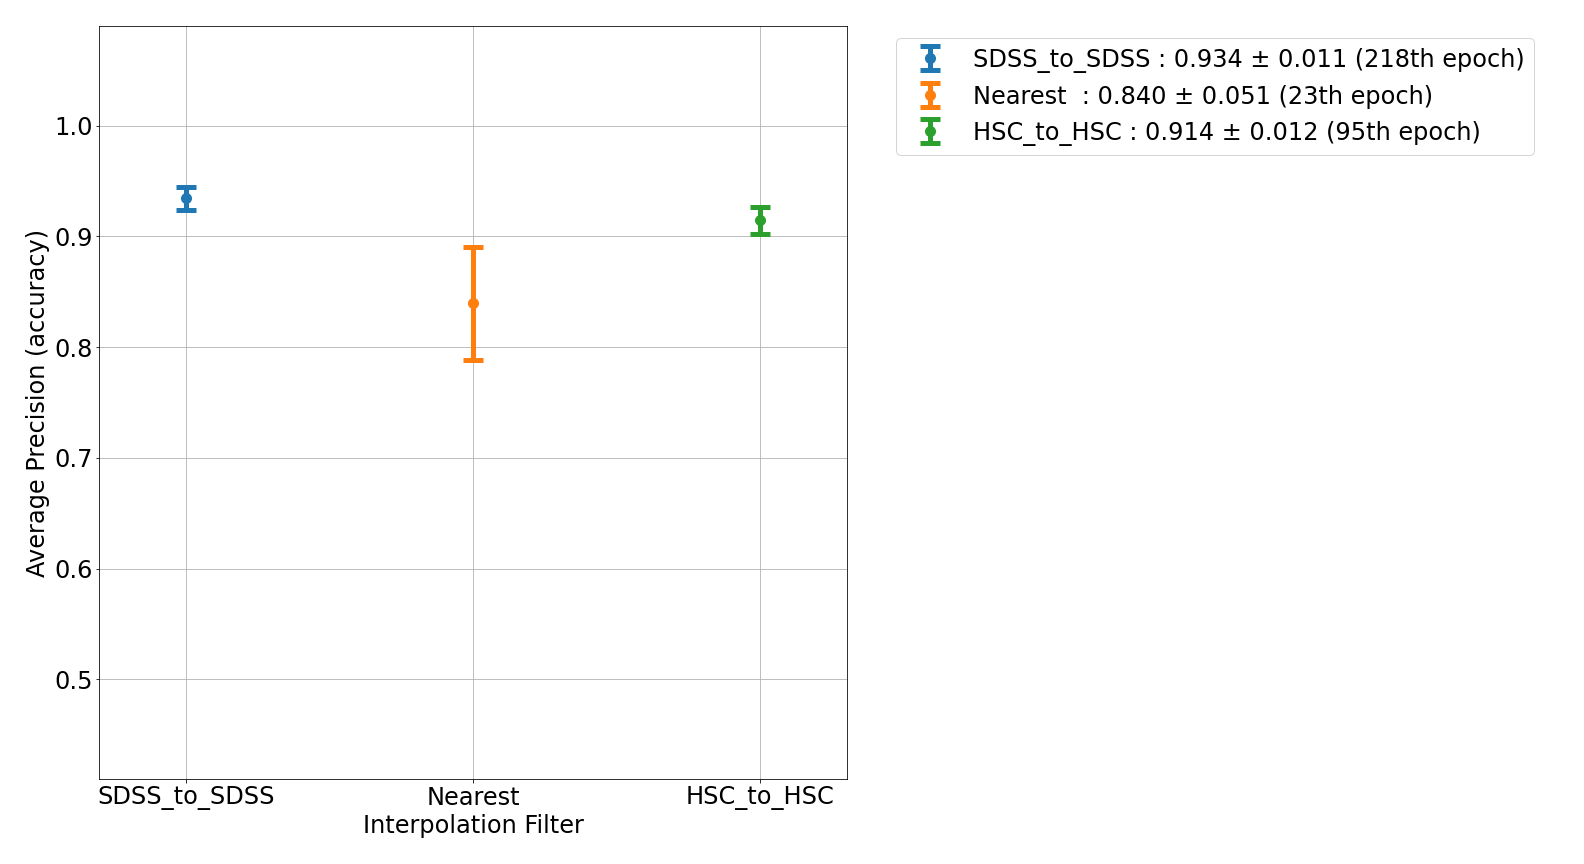
\includegraphics[width=1.0\hsize, keepaspectratio]{images/6syou/acc_with_errorbar_auto_epoch.png}
  \caption{HSCで学習,SDSSに対しテストを行った結果(accuracyの平均値(1標準偏差))}
  \label{fig:6syou_zikkenn}
\end{figure}

\subsection{結果}
hsc$\to$hscの予測精度より,sdss$\to$sdssの予測精度の方が高い.すなわち,高解像度データによって学習したモデルの予測より,低解像度データで学習したモデルの予測の方が結果が良くなっている.

この原因として,2つの原因が考えられる.\\
・GZ1の形態ラベル付けが間違っている.例として,渦巻銀河に対し楕円銀河というラベルがGZ1でつけられたとする.SDSSの解像度では楕円銀河に見えるが,高解像度であるHSCでは渦巻銀河にしか見えないとき,モデルの学習に支障が生じる.\\
・テストデータへの汎化性能が高く,高解像度画像データから複雑な特徴を学習できるモデルを用いらないと,精度が低くなる可能性.




\newpage
\chapter{おわりに}


% END:本編----------------------------------------

% START:参考文献----------------------------------
%% ベタ打ちの場合
% \begin{thebibliography}{1}
% \bibitem{key1}サイト名\\ \url{http://google.com} (yyyy年mm月dd日アクセス) % ウェブサイトの場合
% \bibitem{key2}著者,書籍タイトル,出版                                      % 書籍,論文の場合
% \end{thebibliography}


%% bibtexを使用する場合
\newpage
\bibliography{Master_thesis_bib}         % .bibファイルから拡張子を外した名前 ex)ref.bib
\bibliographystyle{junsrt} % 参考文献出力スタイル
\nocite{*}                 % 参照していない項目も出力する
% END:参考文献------------------------------------


\newpage
\chapter*{謝辞}
本研究を進めるにあたり,ご指導を頂いた飯田佑輔准教授および東京理科大学の大井渚様,そしてデータセット作成や宇宙関連知識取得に際し甚大な助力をいただいた同研究室の津田様に,厚く感謝申し上げます.\\
また,日常の議論を通じて多くの知識や示唆を頂いた飯田佑輔研究室の皆様に感謝いたします.

SDSSおよびSDSS-IIの資金はアルフレッド・P・スローン財団から提供され,また参加機関は米国科学財団,米国エネルギー省,米国航空宇宙局,日本の文部科学省,マックスプランク協会,英国高等教育基金協会です.SDSSのWebサイトは,http://www.sdss.org/ です. 

SDSSは参加機関のための天体物理学研究コンソーシアムによって運営されています.参加機関は,アメリカ自然史博物館,ポツダム天体物理学研究所,バーゼル大学,ケンブリッジ大学,ケース・ウェスタン・リザーブ大学,シカゴ大学,ドレクセル大学,フェルミラボ社,高等研究所,日本参加グループ,ジョンズ・ホプキンス大学,原子核宇宙物理学合同研究所,カブリ粒子宇宙物理学研究所,韓国科学者グループ,中国科学者グループ,中国科学者グループ,韓国科学者グループ 韓国科学者グループ,中国科学院(LAMOST),ロスアラモス国立研究所,マックスプランク天文学研究所,マックスプランク天体物理学研究所,ニューメキシコ州立大学,オハイオ州立大学,ピッツバーグ大学,ポーツマス大学,プリンストン大学,米国海軍天文台,ワシントン大学です.

\end{document}
%------------------------------------------------
